%\documentclass[a4paper,11pt]{book}
\documentclass[a4paper,twoside,12pt,titlepage]{book}
\usepackage[none]{hyphenat}
\usepackage{listings}
\usepackage[utf8]{inputenc}
\usepackage[spanish,es-tabla]{babel}
\usepackage{listings}
\usepackage{xcolor}
\usepackage{amsmath}
\usepackage{eurosym}
\sloppy
\lstset { %
    language=C++,
    backgroundcolor=\color{black!5}, % set backgroundcolor
    basicstyle=\footnotesize,% basic font setting
}
\usepackage{tikz}
\def\checkmark{\tikz\fill[scale=0.4](0,.35) -- (.25,0) -- (1,.7) -- (.25,.15) -- cycle;} 

% \usepackage[style=list, number=none]{glossary} %
%\usepackage{titlesec}
%\usepackage{pailatino}

\decimalpoint
\usepackage{dcolumn}
\newcolumntype{.}{D{.}{\esperiod}{-1}}
\makeatletter
\addto\shorthandsspanish{\let\esperiod\es@period@code}
\makeatother


%\usepackage[chapter]{algorithm}
\RequirePackage{verbatim}
%\RequirePackage[Glenn]{fncychap}
\usepackage{fancyhdr}
\usepackage{graphicx}
\usepackage{afterpage}

\usepackage{longtable}

\usepackage{pythonhighlight}

\usepackage[pdfborder={000}]{hyperref} %referencia

% ********************************************************************
% Re-usable information
% ********************************************************************
\newcommand{\myTitle}{TITULO PROYECTO\xspace}
\newcommand{\myDegree}{Máster en Ingeniería Informática\xspace}
\newcommand{\myName}{Adrián Bonel Bolívar\xspace}
\newcommand{\myProf}{Alvaro Gomez Pau\xspace}
%\newcommand{\mySupervisor}{Put name here\xspace}
%\newcommand{\myFaculty}{Universitat Oberta de Catalunya\xspace}
%\newcommand{\myFacultyShort}{UOC\xspace}
%\newcommand{\myDepartment}{Departamento de Arquitectura y Tecnología de Computadores\xspace}
\newcommand{\myUni}{\protect{Universitat Oberta de Catalunya}\xspace}
\newcommand{\myLocation}{La Llagosta\xspace}
\newcommand{\myTime}{\today\xspace}
\newcommand{\myVersion}{Version 0.1\xspace}


\hypersetup{
pdfauthor = {\myName abonel@uoc.edu},
pdftitle = {\myTitle},
pdfsubject = {},
pdfkeywords = {},
pdfcreator = {LaTeX con VS Code},
pdfproducer = {pdflatex}
}

%\hyphenation{}


%\usepackage{doxygen/doxygen}
%\usepackage{pdfpages}
\usepackage{url}
\usepackage{colortbl,longtable}
\usepackage[stable]{footmisc}
%\usepackage{index}

%\makeindex
%\usepackage[style=long, cols=2,border=plain,toc=true,number=none]{glossary}
% \makeglossary

% Definición de comandos que me son tiles:
%\renewcommand{\indexname}{Índice alfabético}
%\renewcommand{\glossaryname}{Glosario}

\pagestyle{fancy}
\fancyhf{}
\fancyhead[LO]{\leftmark}
\fancyhead[RE]{\rightmark}
\fancyhead[RO,LE]{\textbf{\thepage}}
\renewcommand{\chaptermark}[1]{\markboth{\textbf{#1}}{}}
\renewcommand{\sectionmark}[1]{\markright{\textbf{\thesection. #1}}}

\setlength{\headheight}{1.5\headheight}

\newcommand{\HRule}{\rule{\linewidth}{0.5mm}}
%Definimos los tipos teorema, ejemplo y definición podremos usar estos tipos
%simplemente poniendo \begin{teorema} \end{teorema} ...
\newtheorem{teorema}{Teorema}[chapter]
\newtheorem{ejemplo}{Ejemplo}[chapter]
\newtheorem{definicion}{Definición}[chapter]

\definecolor{gray97}{gray}{.97}
\definecolor{gray75}{gray}{.75}
\definecolor{gray45}{gray}{.45}
\definecolor{gray30}{gray}{.94}

\lstset{ frame=Ltb,
     framerule=0.5pt,
     aboveskip=0.5cm,
     framextopmargin=3pt,
     framexbottommargin=3pt,
     framexleftmargin=0.1cm,
     framesep=0pt,
     rulesep=.4pt,
     backgroundcolor=\color{gray97},
     rulesepcolor=\color{black},
     %
     stringstyle=\ttfamily,
     showstringspaces = false,
     basicstyle=\scriptsize\ttfamily,
     commentstyle=\color{gray45},
     keywordstyle=\bfseries,
     %
     numbers=left,
     numbersep=6pt,
     numberstyle=\tiny,
     numberfirstline = false,
     breaklines=true,
   }
 
% minimizar fragmentado de listados
\lstnewenvironment{listing}[1][]
   {\lstset{#1}\pagebreak[0]}{\pagebreak[0]}

\lstdefinestyle{CodigoC}
   {
	basicstyle=\scriptsize,
	frame=single,
	language=C,
	numbers=left
   }
\lstdefinestyle{CodigoC++}
   {
	basicstyle=\small,
	frame=single,
	backgroundcolor=\color{gray30},
	language=C++,
	numbers=left
   }

 
\lstdefinestyle{Consola}
   {basicstyle=\scriptsize\bf\ttfamily,
    backgroundcolor=\color{gray30},
    frame=single,
    numbers=none
   }


\newcommand{\bigrule}{\titlerule[0.5mm]}

\newcommand*{\captionsource}[2]{
  \caption[{#1}]{
    #1
    %\\\hspace{\linewidth}
    %\centering
    
  }
  \textbf{Fuente:} #2
}



%Para conseguir que en las páginas en blanco no ponga cabecerass
\makeatletter
\def\clearpage{%
  \ifvmode
    \ifnum \@dbltopnum =\m@ne
      \ifdim \pagetotal <\topskip
        \hbox{}
      \fi
    \fi
  \fi
  \newpage
  \thispagestyle{empty}
  \write\m@ne{}
  \vbox{}
  \penalty -\@Mi
}
\makeatother

\usepackage{pdfpages}
\begin{document}
\begin{titlepage}
 
\newlength{\centeroffset}
\setlength{\centeroffset}{-0.5\oddsidemargin}
\addtolength{\centeroffset}{0.5\evensidemargin}
\thispagestyle{empty}

\noindent\hspace*{\centeroffset}\begin{minipage}{\textwidth}

\centering

\includegraphics[width=0.9\textwidth]{imagenes/logo_uoc.png}\\[1.4cm]

\textsc{ \Large TRABAJO FIN DE MÁSTER\\[0.2cm]}
\textsc{ INGENIERÍA INFORMÁTICA}\\[1cm]
% Upper part of the page
% 
% Title
{\Huge\bfseries Monitorización del consumo eléctrico en tiempo real\\
}
\noindent\rule[-1ex]{\textwidth}{3pt}\\[3.5ex]
{\large\bfseries Micropython, Esp32 y MQTT}
\end{minipage}

\vspace{2.5cm}
\noindent\hspace*{\centeroffset}\begin{minipage}{\textwidth}
\centering

\textbf{Autor}\\ {Adrián Bonel Bolívar}\\[2.5ex]
\textbf{Director}\\{Alvaro Gomez Pau}\\[2cm]
%\includegraphics[width=0.3\textwidth]{imagenes/etsiit_logo.png}\\[0.1cm]
\textsc{Sistemas encastados}\\
\textsc{---}\\
Barcelona, Noviembre de 2022
\end{minipage}
%\addtolength{\textwidth}{\centeroffset}
%\vspace{\stretch{2}}
\end{titlepage}



\chapter*{}
%\thispagestyle{empty}
%\cleardoublepage

%\thispagestyle{empty}

%\begin{titlepage}
 
\newlength{\centeroffset}
\setlength{\centeroffset}{-0.5\oddsidemargin}
\addtolength{\centeroffset}{0.5\evensidemargin}
\thispagestyle{empty}

\noindent\hspace*{\centeroffset}\begin{minipage}{\textwidth}

\centering

\includegraphics[width=0.9\textwidth]{imagenes/logo_uoc.png}\\[1.4cm]

\textsc{ \Large TRABAJO FIN DE MÁSTER\\[0.2cm]}
\textsc{ INGENIERÍA INFORMÁTICA}\\[1cm]
% Upper part of the page
% 
% Title
{\Huge\bfseries Monitorización del consumo eléctrico en tiempo real\\
}
\noindent\rule[-1ex]{\textwidth}{3pt}\\[3.5ex]
{\large\bfseries Micropython, Esp32 y MQTT}
\end{minipage}

\vspace{2.5cm}
\noindent\hspace*{\centeroffset}\begin{minipage}{\textwidth}
\centering

\textbf{Autor}\\ {Adrián Bonel Bolívar}\\[2.5ex]
\textbf{Director}\\{Alvaro Gomez Pau}\\[2cm]
%\includegraphics[width=0.3\textwidth]{imagenes/etsiit_logo.png}\\[0.1cm]
\textsc{Sistemas encastados}\\
\textsc{---}\\
Barcelona, Noviembre de 2022
\end{minipage}
%\addtolength{\textwidth}{\centeroffset}
%\vspace{\stretch{2}}
\end{titlepage}






\cleardoublepage
\thispagestyle{empty}

\begin{center}
{\large\bfseries Monitorización del consumo eléctrico en tiempo real}\\
\end{center}
\begin{center}
Adrián Bonel Bolívar\\
\end{center}

%\vspace{0.7cm}
\noindent{\textbf{Palabras clave}: Micropython, Software embebido, Esp32, Acs712, ZMPT101B, MQTT, Flask, Python, App Web}\\

\vspace{0.7cm}
\noindent{\textbf{Resumen}}\\

A día de hoy, el coste de la electricidad ha aumentado a unos niveles que nadie hubiera imaginado hace tan solo unos años. Muchas familias cada vez más, necesitan ir con mucho cuidado sobre cuándo poner ciertos electrodomésticos en casa, para elegir la hora donde el precio está más bajo y así poder ahorrar en la factura de la luz. Saber cuánto consume cada electrodoméstico y como se refleja en el coste de la factura puede llegar a ser de gran utilidad. \\

Aquí es donde podemos situar el trabajo de este proyecto. Aunque a día de hoy existen sistemas inteligentes con los que gestionar y monitorizar la energía que se consume en el hogar, normalmente estos dispositivos son independientes unos de otros y no encontramos muchos que recopilen los datos. El trabajo de este proyecto, no solo se va a centrar en medir el consumo eléctrico de los dispositivos individualmente, si no que el objetivo será que toda esa información se pueda consultar desde una misma aplicación. \\

Planteamos por tanto el despliegue de sistemas embebidos capaces de medir el consumo eléctrico y que a su vez sean capaces de comunicarse con un servidor central donde recopilar todos los datos. El despliegue de estos sistemas se hará en un entorno real, donde se probará el funcionamiento de los dispositivos y se analizará el rendimiento de los mismos. \\

\cleardoublepage


\thispagestyle{empty}


\begin{center}
{\large\bfseries Real time measurement of power consumption}\\
\end{center}
\begin{center}
Adrián Bonel Bolívar\\
\end{center}

%\vspace{0.7cm}
\noindent{\textbf{Keywords}: Micropython, Embedded software, Esp32, Acs712, ZMPT101B, MQTT, Flask, Python, Web app}\\

\vspace{0.7cm}
\noindent{\textbf{Abstract}}\\

Today, the cost of electricity has risen to levels that no one would have imagined just a few years ago. Increasingly, many families need to be very careful about when to put certain devices in the house, to choose the time when the price is lower and thus be able to save on the electricity bill. Knowing how much each device consumes and how it is reflected in the cost of the bill can be very useful. \\

This is where we can place the work of this project. Although today there are intelligent systems with which to manage and monitor the energy consumed in the home, these devices are usually independent of each other and we do not find many that collect the data. The work of this project will not only focus on measuring the power consumption of individual devices, but the goal will be that all this information can be consulted from a single application. \\

We therefore propose the deployment of embedded systems capable of measuring electricity consumption and at the same time be able to communicate with a central server to collect all the data. The deployment of these systems will be done in a real environment, where the operation of the embedded systems will be tested and their performance will be analyzed. \\

\chapter*{}
\thispagestyle{empty}

\noindent\rule[-1ex]{\textwidth}{2pt}\\[4.5ex]

Yo, \textbf{Adrián Bonel Bolívar}, alumno del Máster en Ingeniería Informática de la \textbf{Universitat Oberta de Catalunya}, con DNI 76668939A, autorizo la
ubicación de la siguiente copia de mi Trabajo Fin de Máster en la biblioteca del centro para que pueda ser
consultada por las personas que lo deseen.

\vspace{6cm}

\noindent Fdo: Adrián Bonel Bolívar

\vspace{2cm}

\begin{flushright}
Barcelona a 30 de Noviembre de 2022.
\end{flushright}


%\chapter*{Agradecimientos}
%\thispagestyle{empty}

%       \vspace{1cm}


%Inventar cosas aqui





\frontmatter
\tableofcontents
\listoffigures
%\listoftables
\setcounter{section}{0}
%
\mainmatter
\setlength{\parskip}{5pt}

%
\begin{titlepage}

\chapter{Introducción}
\section{Introducción y motivación}
A día de hoy, el coste de la electricidad ha aumentado a unos niveles que nadie hubiera imaginado hace tan solo unos años. Muchas familias cada vez más, necesitan ir con mucho cuidado sobre cuándo poner ciertos electrodomésticos en casa, para elegir la hora donde el precio está más bajo y así poder ahorrar en la factura de la luz. Saber cuánto consume cada electrodoméstico y como se refleja en el coste de la factura puede llegar a ser de gran utilidad. \\

Y aquí es donde podemos situar el trabajo de este proyecto. Aunque a día de hoy existen sistemas inteligentes con los que gestionar y monitorizar la energía que se consume en el hogar, normalmente estos dispositivos son independientes unos de otros y no encontramos muchos que recopilen los datos. Estos dispositivos que ya existen en el mercado los analizaremos más adelante. El trabajo de este proyecto, no solo se va a centrar en medir el consumo eléctrico de los dispositivos individualmente, si no que el objetivo será que toda esa información se pueda consultar desde una misma aplicación. \\

En este proyecto se plantea el despliegue de diferentes sistemas embebidos que sean capaces de calcular el consumo energético de los dispositivos conectados y que envíen esos datos por MQTT. Una aplicación web será la encargada de recopilar los datos de todos los dispositivos y de mostrar toda la información posible en relación al consumo energético.\\

\section{Objetivos}

\begin{enumerate}
\item Estudio de viabilidad de la plataforma de desarrollo. Uso de micropython y estudio de la existencia de librerias para la comunicación inalámbrica por MQTT.
\item Estudio de los diferentes dispositivos que se pueden utilizar para medir el consumo eléctrico. 
\item Puesta a punto de Raspberry Pi para el despliegue de un broker MQTT.
\item Integración de los sensores y dispositivos con la plataforma elegida.
\item Aplicación web en Flask que permita la visualización de los datos recogidos por los dispositivos en tiempo real.
\end{enumerate}

\section{Planificación}
La planificación inicial y el tiempo estimado a emplear en cada tarea fue el siguiente:
\begin{figure}[h!]
	\centering
	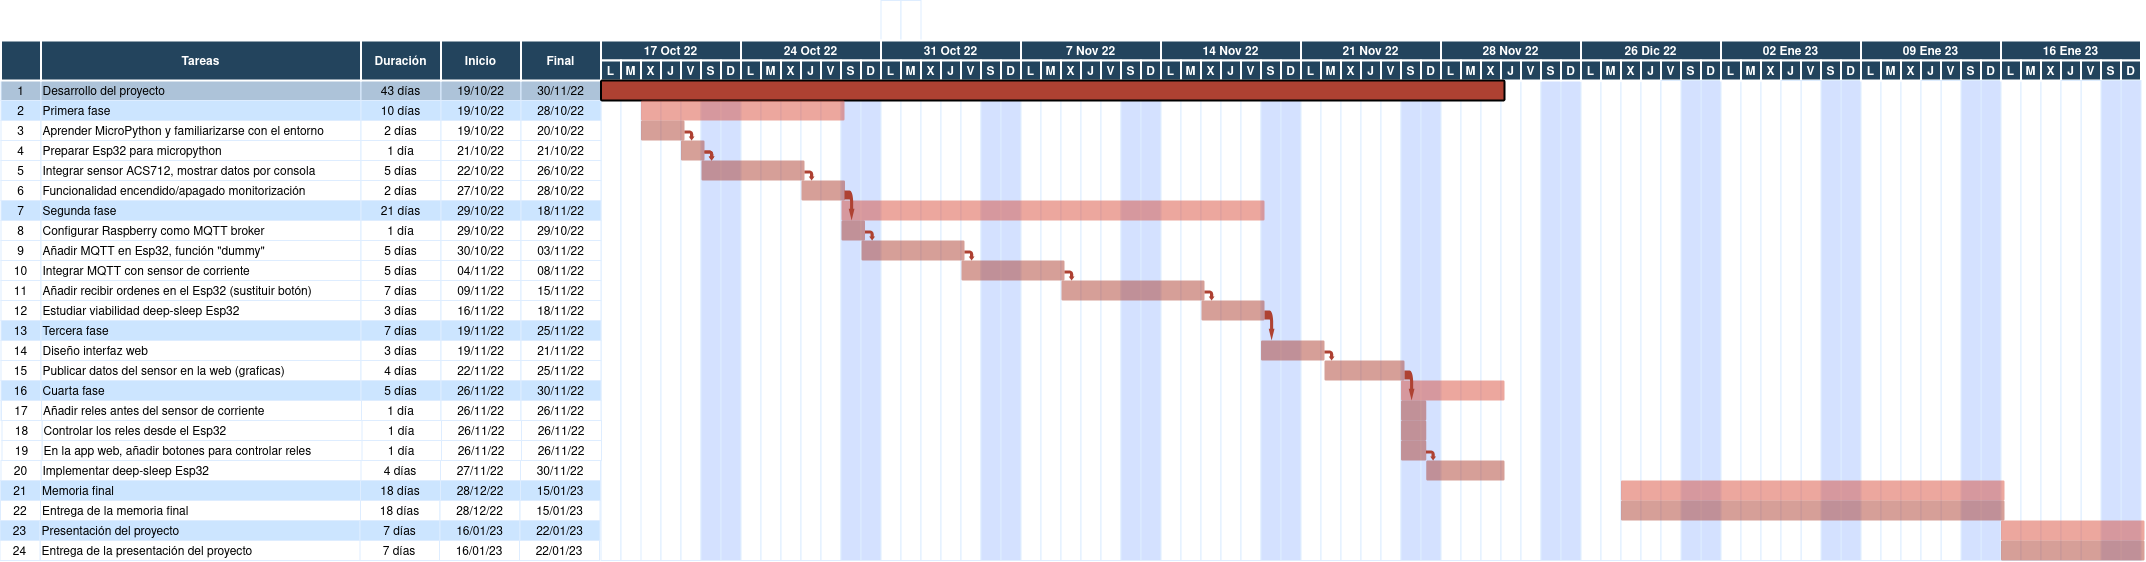
\includegraphics[width=1\textwidth]{imagenes/gantt_inicial.PNG}
	\caption{Diagrama de Gantt para la planificación inicial}
\end{figure}
Hasta el momento, se han cumplido la mayoría de objetivos planificados, aunque se han tenido que retrasar algunas tareas debido a la falta de tiempo. A continuación se muestra la planificación actualizada:

\begin{figure}[h!]
	\centering
	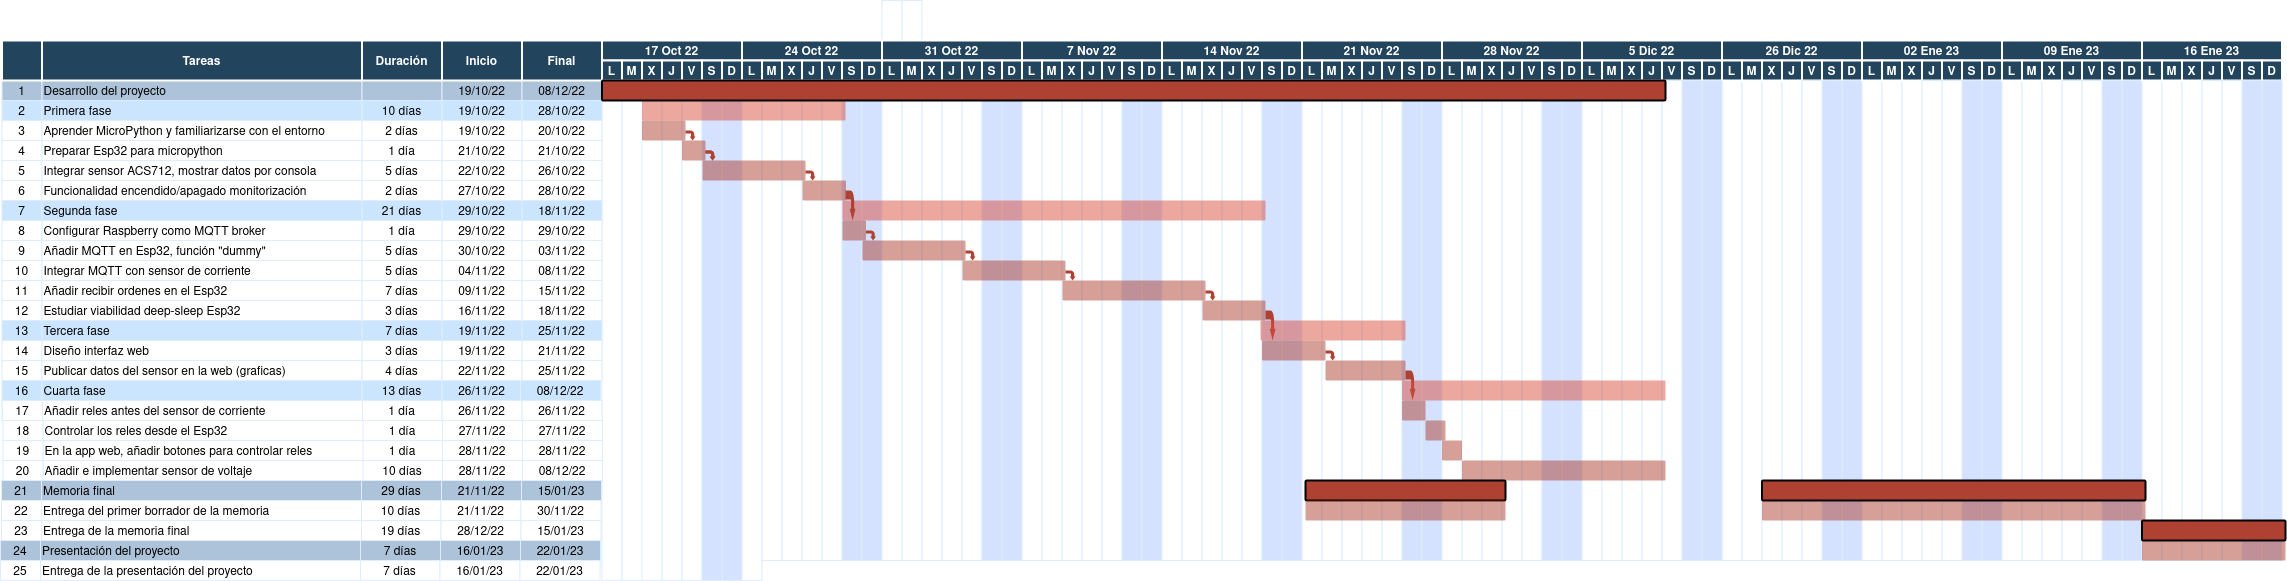
\includegraphics[width=1\textwidth]{imagenes/gantt_final.PNG}
	\caption{Diagrama de Gantt de la planificación final}
\end{figure}

\newpage
\section{Material y métodos}

Para el desarrollo del sistema embebido, se ha utilizado el lenguaje de programación Micropython, que veremos más en detalle más adelante. La aplicación web ha sido desarrollada en python haciendo uso de librerias como Flask.\\

Para la creación de este documento se ha utilizado Texmaker como plataforma de creación y edición de documentos \LaTeX .\\

\subsubsection{Software}
\begin{itemize}
	\item Visual Studio Code como IDE de programación.
	\item Ordenador con Ubuntu como sistema operativo.
	\item Esptool como herramienta para trabajar con la flash de los ESP32.
	\item Picocom como software para la comunicación por serial.
	\item Ampy de Adafruit como herramienta para cargar ficheros en los ESP32.
	\item Tauno serial plotter para la visualización de los datos recibidos por el puerto serie.
	\item Git para el control de versiones.
\end{itemize}

\subsubsection{Equipos}
\begin{itemize}
	\item Raspberry Pi 2B+ como broker MQTT.
	\item x3 ESP32.
	\item x3 sensores de corriente ACS712.
	\item x3 sensores de voltaje. 
	\item x3 pantallas OLED SSD1306.
	\item x3 cables USB - Micro USB.
	\item x3 reles.
	\item Multímetro
	\item Fuente de alimentación.
	\item x6 Mini breadboards.
	\item Otros componentes electrónicos.
\end{itemize}

\section{Estructura del documento}
El documento se divide en 5 capítulos, que se describen a continuación:
\begin{enumerate}
\item Capítulo 1. Introducción. En este capítulo se describen los objetivos del proyecto, así como la planificación inicial y la planificación actualizada. También se describen los materiales y métodos utilizados para la realización del proyecto. 
\item Capítulo 2. Estudio del problema. En este capítulo se describen los diferentes dispositivos que se pueden utilizar para medir el consumo eléctrico. También se describen los diferentes protocolos de comunicación que se pueden utilizar entre los dispositivos y el servidor.
\item Capítulo 3. Implementación del sistema de monitorización de corriente. En este capítulo se describe la solución final, los materiales utilizados, el setup experimental y la implementación en Micropython.
\item Capítulo 4. Despliegue del broker MQTT. En este capítulo se describe la instalación y configuración del broker MQTT en Raspberry Pi.
\item Capítulo 5. Implementación de la aplicación web. En este capítulo se describe la implementación de la aplicación web en Python usando Flask, SocketIO y MQTT.
\item Capítulo 6. Conclusiones y trabajo futuro. En este capítulo se describen las conclusiones del proyecto y las posibles mejoras que se podrían realizar en el futuro.
\end{enumerate}

\end{titlepage}

%
\begin{titlepage}

\chapter{Fundamentación teórica}
\section{Consumo energético}
\subsection{Consumo energético en el hogar}
\subsubsection{Contadores inteligentes}
A día de hoy la mayoría de las compañías eléctricas están sustituyendo los contadores en todas las viviendas por nuevos contadores inteligentes que te muestran el consumo eléctrico de toda la vivienda en tiempo real.\\

Ventajas:
\begin{itemize}
	\item En teoría, la renovación de los contadores corre a cargo de las compañías eléctricas, por lo que esta opción no tiene ningún coste extra.
\end{itemize}
Inconvenientes:
\begin{itemize}
	\item La medida que nos da es genérica y no podemos saber cual es el consumo individual de ciertos dispositivos en nuestra red.
	\item En algunos bloques de viviendas, los contadores no se encuentran dentro de las viviendas si no en zonas comunes, por lo que no es tan fácil consultar los datos.
\end{itemize}
\begin{figure}[h!]
	\centering
	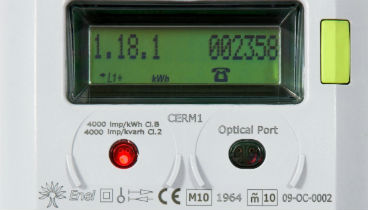
\includegraphics[width=0.75\textwidth]{imagenes/contador.jpg}
	\caption{Contador de luz\cite{contador_img}}
\end{figure}
\subsubsection{Factura de la luz}
En la factura eléctrica podemos consultar el desglose del consumo general por tramos.\\

Ventajas:
\begin{itemize}
	\item Desglose por tarifas del consumo.
\end{itemize}
Inconvenientes:
\begin{itemize}
	\item No podemos conocer en tiempo real el consumo eléctrico de la vivienda.
	\item No podemos saber cuál es el consumo individual de dispositivos en nuestra red.
\end{itemize}
%\begin{figure}[h!]
%	\centering
%	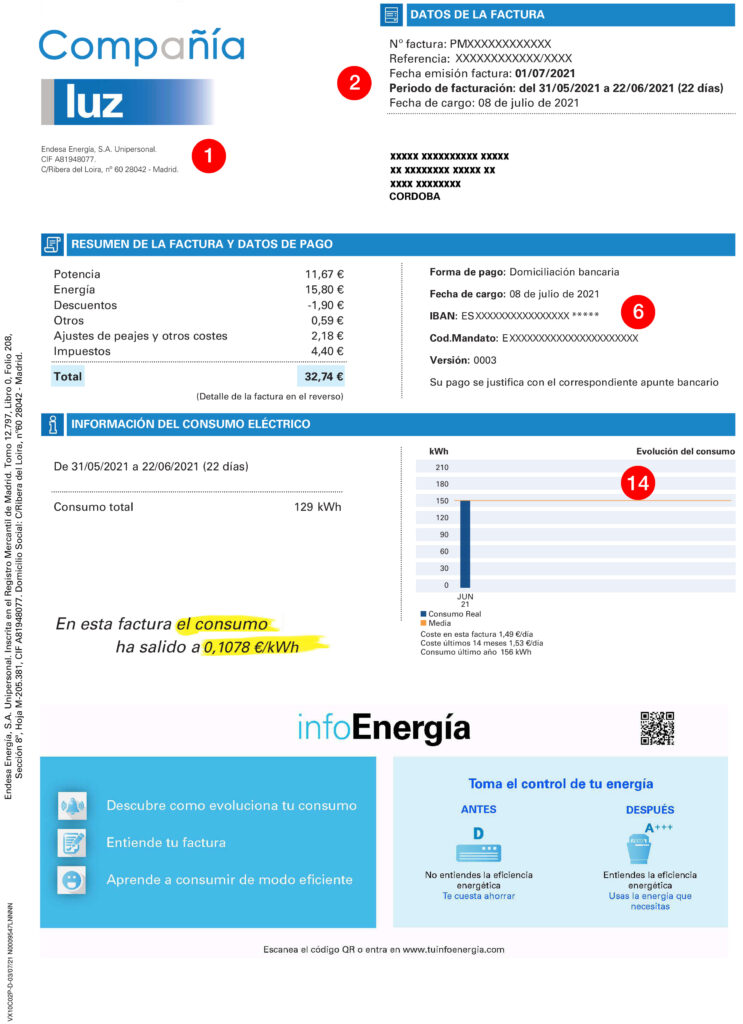
\includegraphics[width=1\textwidth]{imagenes/factura_luz.jpg}
%	\caption{Ejemplo factura de la luz\cite{factura_img}}
%\end{figure}

\subsubsection{Calculo manual del consumo}
Podemos calcular cuánto gasta un dispositivo de manera fácil conociendo su potencia y el tiempo que está encendido. Mas adelante veremos mas en profundidad como hacerlo de diferentes formas.\\

Inconvenientes:\\
\begin{itemize}
	\item Solo es posible saber el consumo teórico.
\end{itemize}

\subsubsection{Medidor de consumo electrico individual}
Medidor de consumo para monitorizar la energía de un dispositivo conectado a la red eléctrica.\\

Ventajas:
\begin{itemize}
	\item Protección por sobrecarga eléctrica incorporado.
	\item Pantalla incorporada para mostrar la lectura.
\end{itemize}

Inconvenientes:
\begin{itemize}
	\item No es posible utilizar los datos de consumo fuera de la pantalla incorporada.
	\item No es posible consultar un historico de consumo.
\end{itemize}
\begin{figure}[h!]
	\centering
	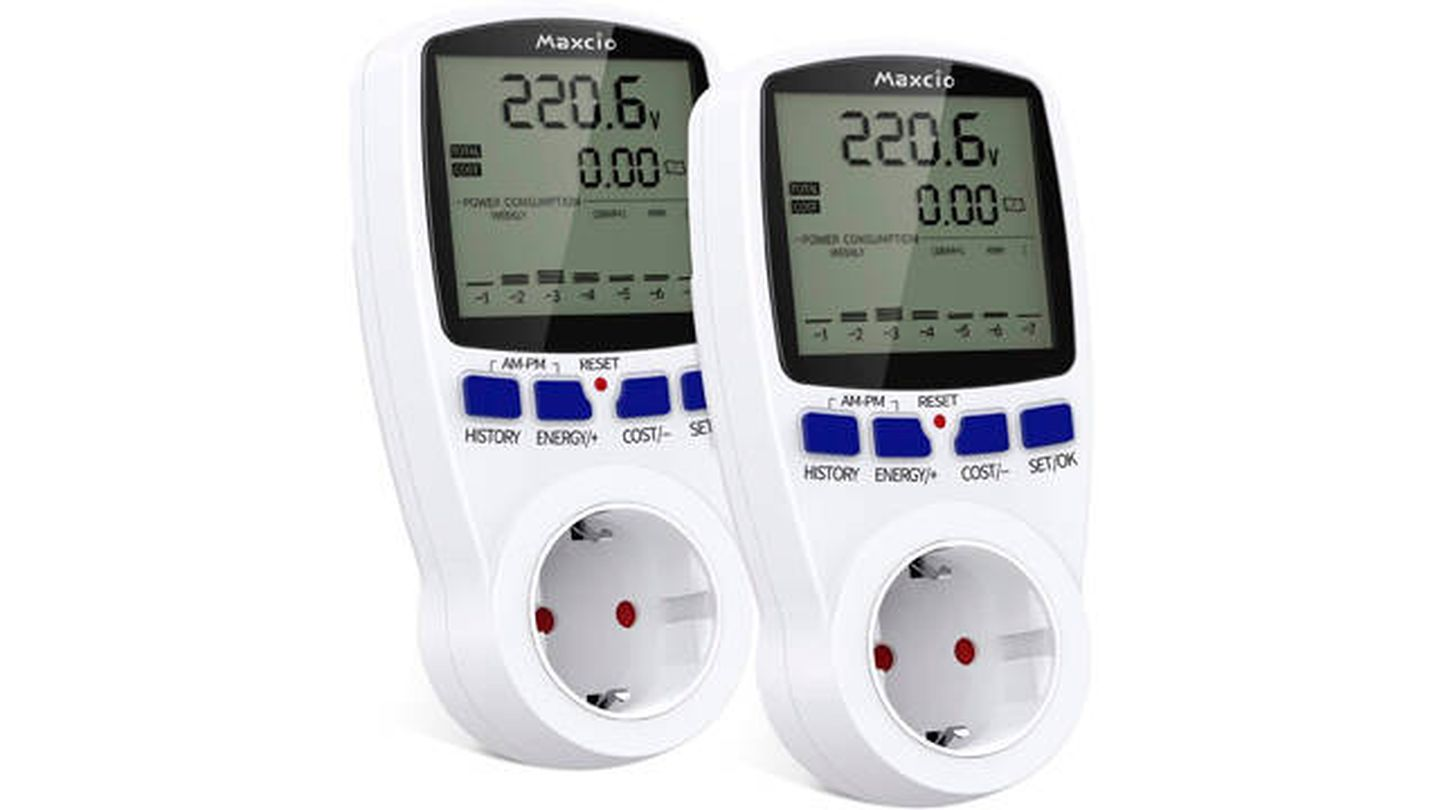
\includegraphics[width=0.5\textwidth]{imagenes/medidor_consumo.jpg}
	\caption{Medidor de consumo de energía\cite{medidor_img}}
\end{figure}

\subsubsection{Medidor cuadro electrico}
Permite medir la energía eléctrica de manera precisa y fiable.\\

Ventajas:
\begin{itemize}
	\item Está pensado para instalarse directamente en el cuadro eléctrico.
	\item Permite medir amperajes muy altos.
\end{itemize}

Inconvenientes:
\begin{itemize}
	\item Al instalarse en el cuadro eléctrico, la medida que nos da es genérica y no podemos saber cual es el consumo individual de ciertos dispositivos en nuestra red electrica. 
\end{itemize}
\begin{figure}[h!]
	\centering
	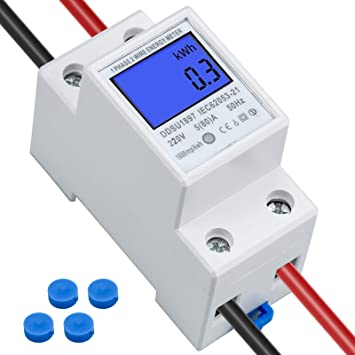
\includegraphics[width=0.25\textwidth]{imagenes/medidor_cuadro.jpg}
	\caption{Medidor de consumo en cuadro electrico\cite{medidor_cuadro_img}}
\end{figure}

\subsubsection{Monitor inteligente de energia}
Sistema que agrega sensores individuales para monitorizar de forma precisa electrodomésticos y otros tipos de dispositivos. Integración con una app Android para consultar los datos. Esta opción sería lo más parecido al sistema que este proyecto plantea.\\

Ventajas:
\begin{itemize}
	\item Sensores de hasta 50A.
	\item Cuenta con una aplicación para consultar los datos de cada sensor.
\end{itemize}

Inconvenientes:
\begin{itemize}
	\item Los sensores se comunican con el panel principal por cable.
	\item Coste elevado.
\end{itemize}
\begin{figure}[h!]
	\centering
	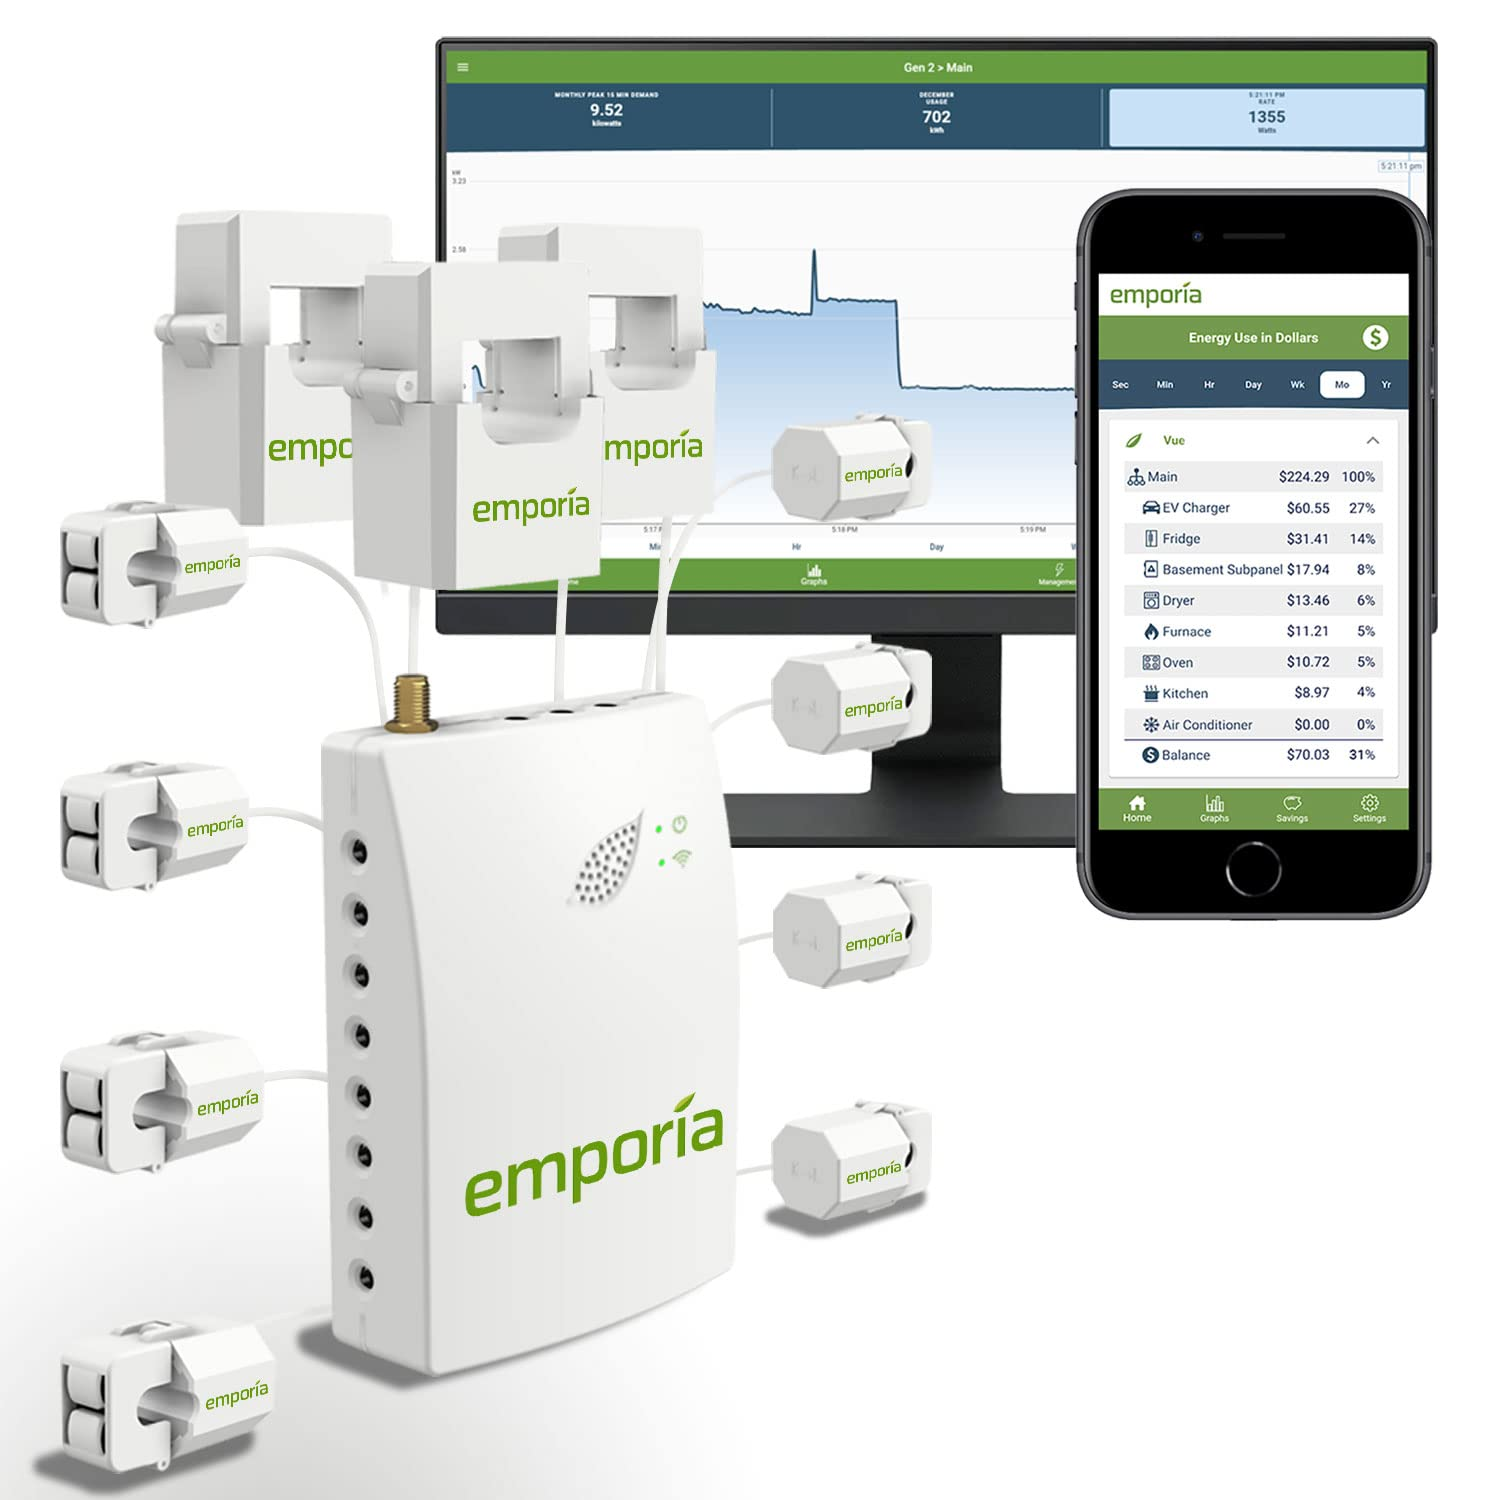
\includegraphics[width=0.25\textwidth]{imagenes/monitor_consumo.jpg}
	\caption{Monitor de energia inteligente\cite{monitor_inteligente_img}}
\end{figure}

\newpage

\subsection{Calculo del consumo energético}
Lo primero que necesitamos entender es como podemos calcular el consumo electrico de cualquier dispositvo. Sabiendo los datos teoricos, es algo bastante simple, tan solo necesitamos aplicar la siguiente formula: \\
\begin{equation}
\label{eq:consumo}
P = I \cdot V
\end{equation}

Donde P es el consumo en vatios, I es la intensidad en amperios y V es la tensión en voltios. La tensión es facil saberla. En España y en la mayoria de paises europeos, la tensión es de 230V. Pero la intensidad es algo mas complicado. Para saber la intensidad necesitamos saber la potencia del dispositivo. Para ello, podemos consultar la etiqueta de consumo de cada dispositivo. En la etiqueta de consumo, podemos ver la potencia en vatios, la intensidad en amperios y la tensión en voltios. Pero esta potencia que nos indica el dispositivo no es la real. Normalmente es la potencia maxima que puede llegar a consumir el dispositivo, pero no la que realmente consume. Para calcular la potencia real, podemos hacer uso de un multimetro y asi obtener la intensidad real, y con esto calcular la potencia que consume. En nuestra solución no podremos hacer uso de un multimetro, asi que necesitamos entender como hace el multimetro para calcular la intensidad. \\

\subsubsection{Onda sinusoidal}
La corriente alterna viaja por el cableado en formas de ondas Sinusoidales. La forma de onda de la corriente alterna es la siguiente: \\ 

\begin{figure}[h!]
	\centering
	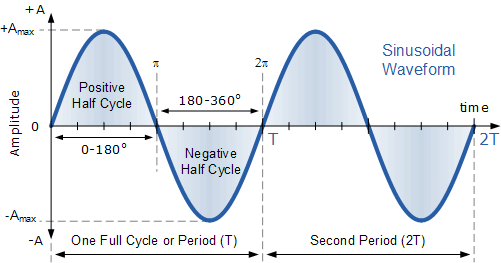
\includegraphics[width=0.75\textwidth]{imagenes/sine_wave.png}
	\caption{Forma de una onda Sinusoidal\cite{sine_wave_img}}
\end{figure}
\newpage
Aquí podemos diferenciar tres caracteristicas de la onda sinusoidal\cite{ref2}: \\
\begin{itemize}
	\item Amplitud: Es la distancia entre el punto mas alto y el mas bajo de la onda. Esta es la intensidad de la señal de corriente.
	\item Frecuencia: Es el numero de veces que la onda se repite en un segundo. En España, la frecuencia es de 50Hz.
	\item Periodo: Es el tiempo que tarda en completarse una onda.
\end{itemize}
Para poder calcular correctamente el consumo de un dispositivo, tenemos que medir correctamente la amplitud de la onda, es decir, el maximo y minimo de la onda. Asi es como los amperimetros y los multimetros calculan la intensidad. \\
\subsubsection{Factor de potencia}
El factor de potencia\cite{ref3} se utiliza como expresión para indicar la relación entre la potencia activa y la potencia aparente. La potencia aparente es la potencia que se mide en el medidor de la compañia electrica. La potencia activa es la potencia que realmente consume el dispositivo. Si un circuito electrico fuera cien por cien eficiente, la potencia activa y la potencia aparente serian iguales. Pero en la realidad, los circuitos no son cien por cien eficientes, y por tanto, la potencia activa es menor que la potencia aparente. \\
\begin{equation}
\label{eq:factor_potencia}
FP = \frac{P_{activa}}{P_{aparente}}
\end{equation}
El factor de potencia es un valor que oscila entre 0 y 1. Cuanto mas cercano a 1, mas eficiente es el circuito. Cuanto mas cercano a 0, menos eficiente es el circuito. En aparatos electricos resistivos (como por ejemplo un radiador), el factor de potencia es muy cercano a 1 ya que convierten toda la energia electrica que reciben en calor. En aparatos electricos inductivos, como por ejemplo un motor, el factor de potencia es mucho mas bajo ya que no convierten toda la energia electrica que reciben en trabajo.

\subsubsection{Media cuadratica (RMS)}
Para este proyecto, no nos interesa el el peak-to-peak de la onda, sino la media cuadratica\cite{ref4} de la onda para poder saber la intensidad continua que consume el dispositivo. Para calcular la media cuadratica, podemos hacer uso de la siguiente formula: \\
\begin{equation}
\label{eq:peak_to_peak}
	V_{peak\_to\_peak} = V_{max} - V_{min}
\end{equation}
	
\begin{equation}
\label{eq:media_cuadratica}
Voltage RMS = (\frac{V_{peak\_to\_peak}}{2}) \cdot \sqrt{2}
\end{equation}

\subsection{Sensores de consumo energético}
A continuacion vamos a ver los diferentes tipos de sensores que podemos utilizar para medir el consumo de un dispositivo en nuestro proyecto. \\
\subsubsection{INA219}
El sensor INA219\cite{ref5} es un sensor de corriente y voltaje de alta precision. Este sensor es capaz de medir hasta 26V. Este sensor es muy util para medir el consumo de un dispositivo, ya que es capaz de medir tanto la intensidad como la tensión, como por ejemplo para monitorizar la duración de baterias.\\

Caracteristicas:
\begin{itemize}
	\item Mide tensiones entre 0 y 26V.
	\item Interfaz de comunicación I2C.
	\item Alta precisión.
	\item Opciones de calibración para ajustar la sensibilidad.
\end{itemize}
\begin{figure}[h!]
	\centering
	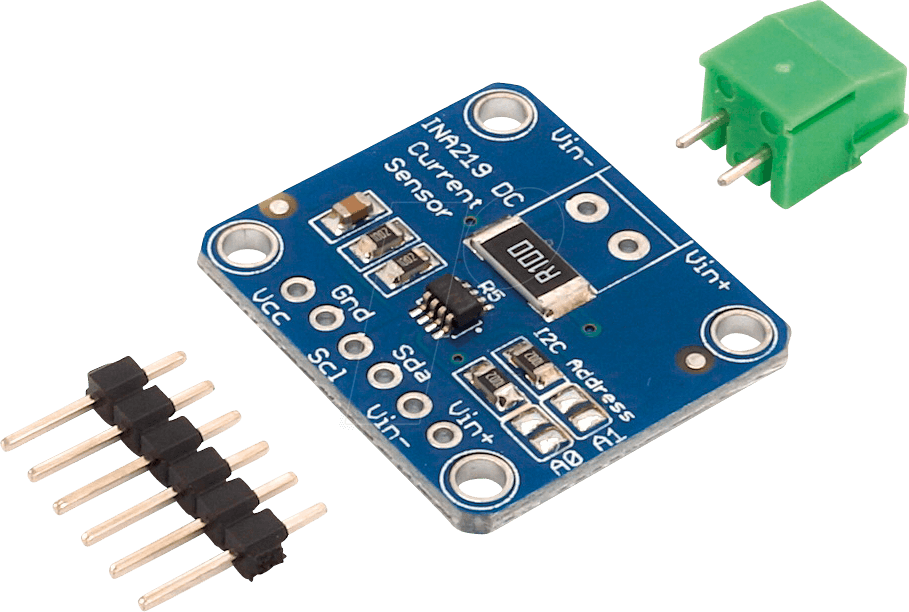
\includegraphics[width=0.25\textwidth]{imagenes/ina219.png}
	\caption{Sensor INA219\cite{ina219_img}}
\end{figure}

\subsubsection{ZMPT101B}
El sensor ZMPT101B\cite{ref6} es capaz de medir hasta 1000V. \\

Caracteristicas:
\begin{itemize}
	\item Alto aislamiento.
	\item Rango amplio
	\item Alta precisión
	\item Resultados estables
\end{itemize}

\begin{figure}[h!]
	\centering
	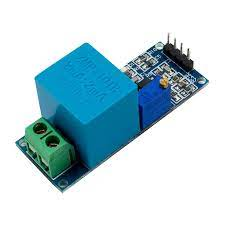
\includegraphics[width=0.25\textwidth]{imagenes/zmpt101b.jpeg}
	\caption{Sensor ZMPT101B\cite{zmpt101b_img}}
\end{figure}


\subsubsection{ACS712}
El sensor ACS712\cite{ref7} es un sensor barato y preciso para medir la corriente tanto continua como alterna. Existen 3 modelos de este sensor, uno para medir corrientes de 5A, otro para medir corrientes de 20A y otro para medir corrientes de 30A. \\

Caracteristicas:
\begin{itemize}
	\item Alta precisión.
	\item Señal de salida con bajo ruido.
\end{itemize}
\begin{figure}[h!]
	\centering
	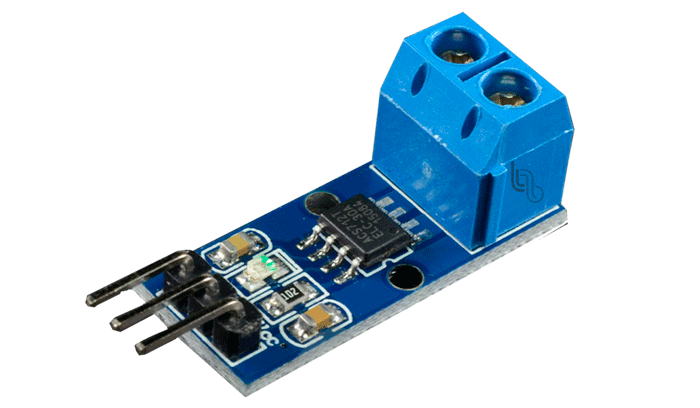
\includegraphics[width=0.25\textwidth]{imagenes/acs712.png}
	\caption{Sensor ACS712\cite{acs712_img}}
\end{figure}

\section{Plataformas de desarrollo}
Para este proyecto, buscamos una plataforma de desarrollo de software embebido que disponga de ADCs y de una interfaz de comunicación inalámbrica para poder enviar los datos a un servidor. A continuación vamos a ver las diferentes opciones que tenemos. \\
\subsection{Arduino}
Arduino\cite{ref8} es una plataforma de desarrollo de software embebido basada en microcontroladores. Arduino es una plataforma muy popular y tiene una gran comunidad de usuarios. Arduino tiene una gran cantidad de shields, que son placas de expansion que se pueden conectar a la placa base de Arduino. No dispone de WiFi integrado, pero podriamos conectarle un modulo WiFi. El Arduino UNO dispone de 6 entradas analogicas. \\
\begin{figure}[h!]
	\centering
	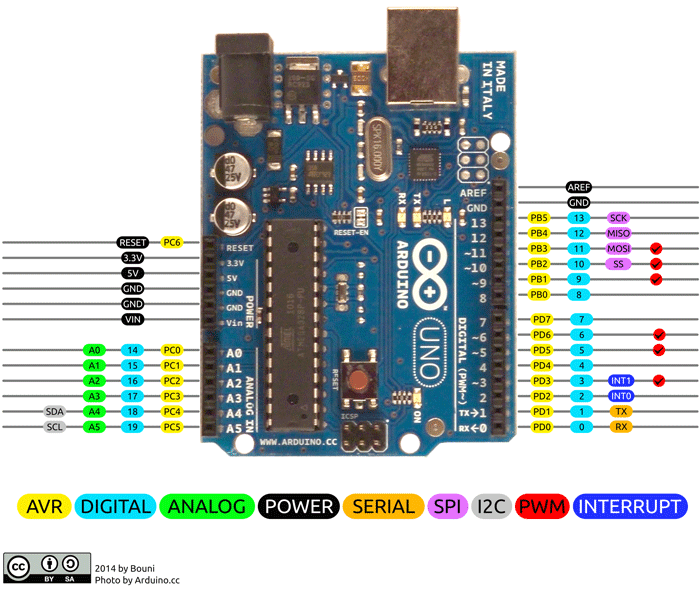
\includegraphics[width=0.5\textwidth]{imagenes/arduino.png}
	\caption{Arduino pin layout\cite{arduino_img}}
\end{figure}
\subsection{Raspberry Pi}
La Raspberry Pi\cite{ref9} es un mini ordenador de bajo coste (aunque mas caro que el resto de plataformas que vamos a ver). No inclute ningun convertidor analogico digital, por lo que tendriamos que usar un modulo externo. Si dispone de WiFi.
\begin{figure}[h!]
	\centering
	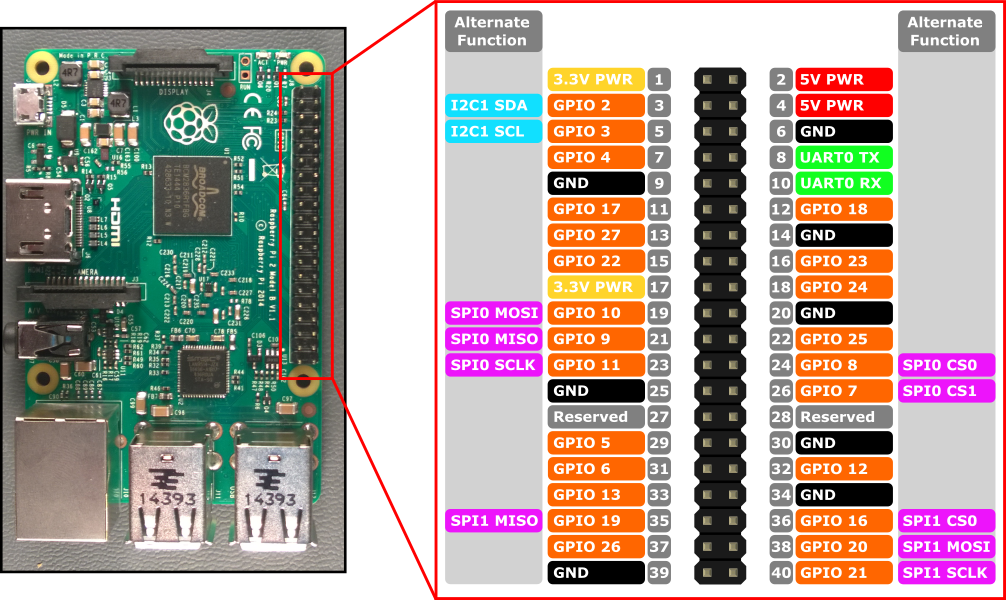
\includegraphics[width=0.5\textwidth]{imagenes/rpi.png}
	\caption{Raspberry Pi pin layout\cite{rpi_img}}
\end{figure}
\subsection{ NodeMCU ESP8266}
El NodeMCU ESP8266\cite{ref10} es una plataforma de codigo abierto que como su propio nombre indica, incluye un modulo WiFi ESP8266. Es un proyecto ya abandonado pero que tiene una gran comunidad de usuarios que lo siguen manteniendo. Esta plataforma tan solo dispone de un ADC, pero de resolución de 10 bits. \\
\begin{figure}[h!]
	\centering
	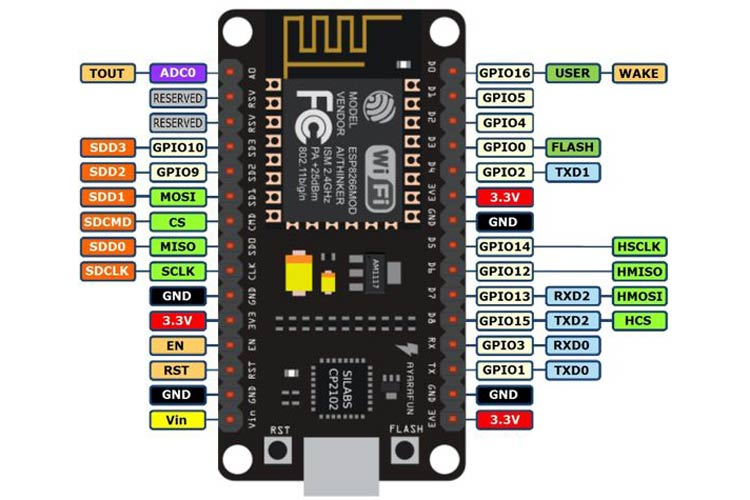
\includegraphics[width=0.5\textwidth]{imagenes/esp8266.jpg}
	\caption{Node MCU ESP8266 pin layout\cite{esp8266_img}}
\end{figure}
\subsection{ESP32}
El ESP32\cite{ref11} es un microcontrolador con WiFi integrado. Dispone de hasta 18 entradas analogicas. Es el sucesor del ESP8266, por lo que es una plataforma mas moderna. \\
\begin{figure}[h!]
	\centering
	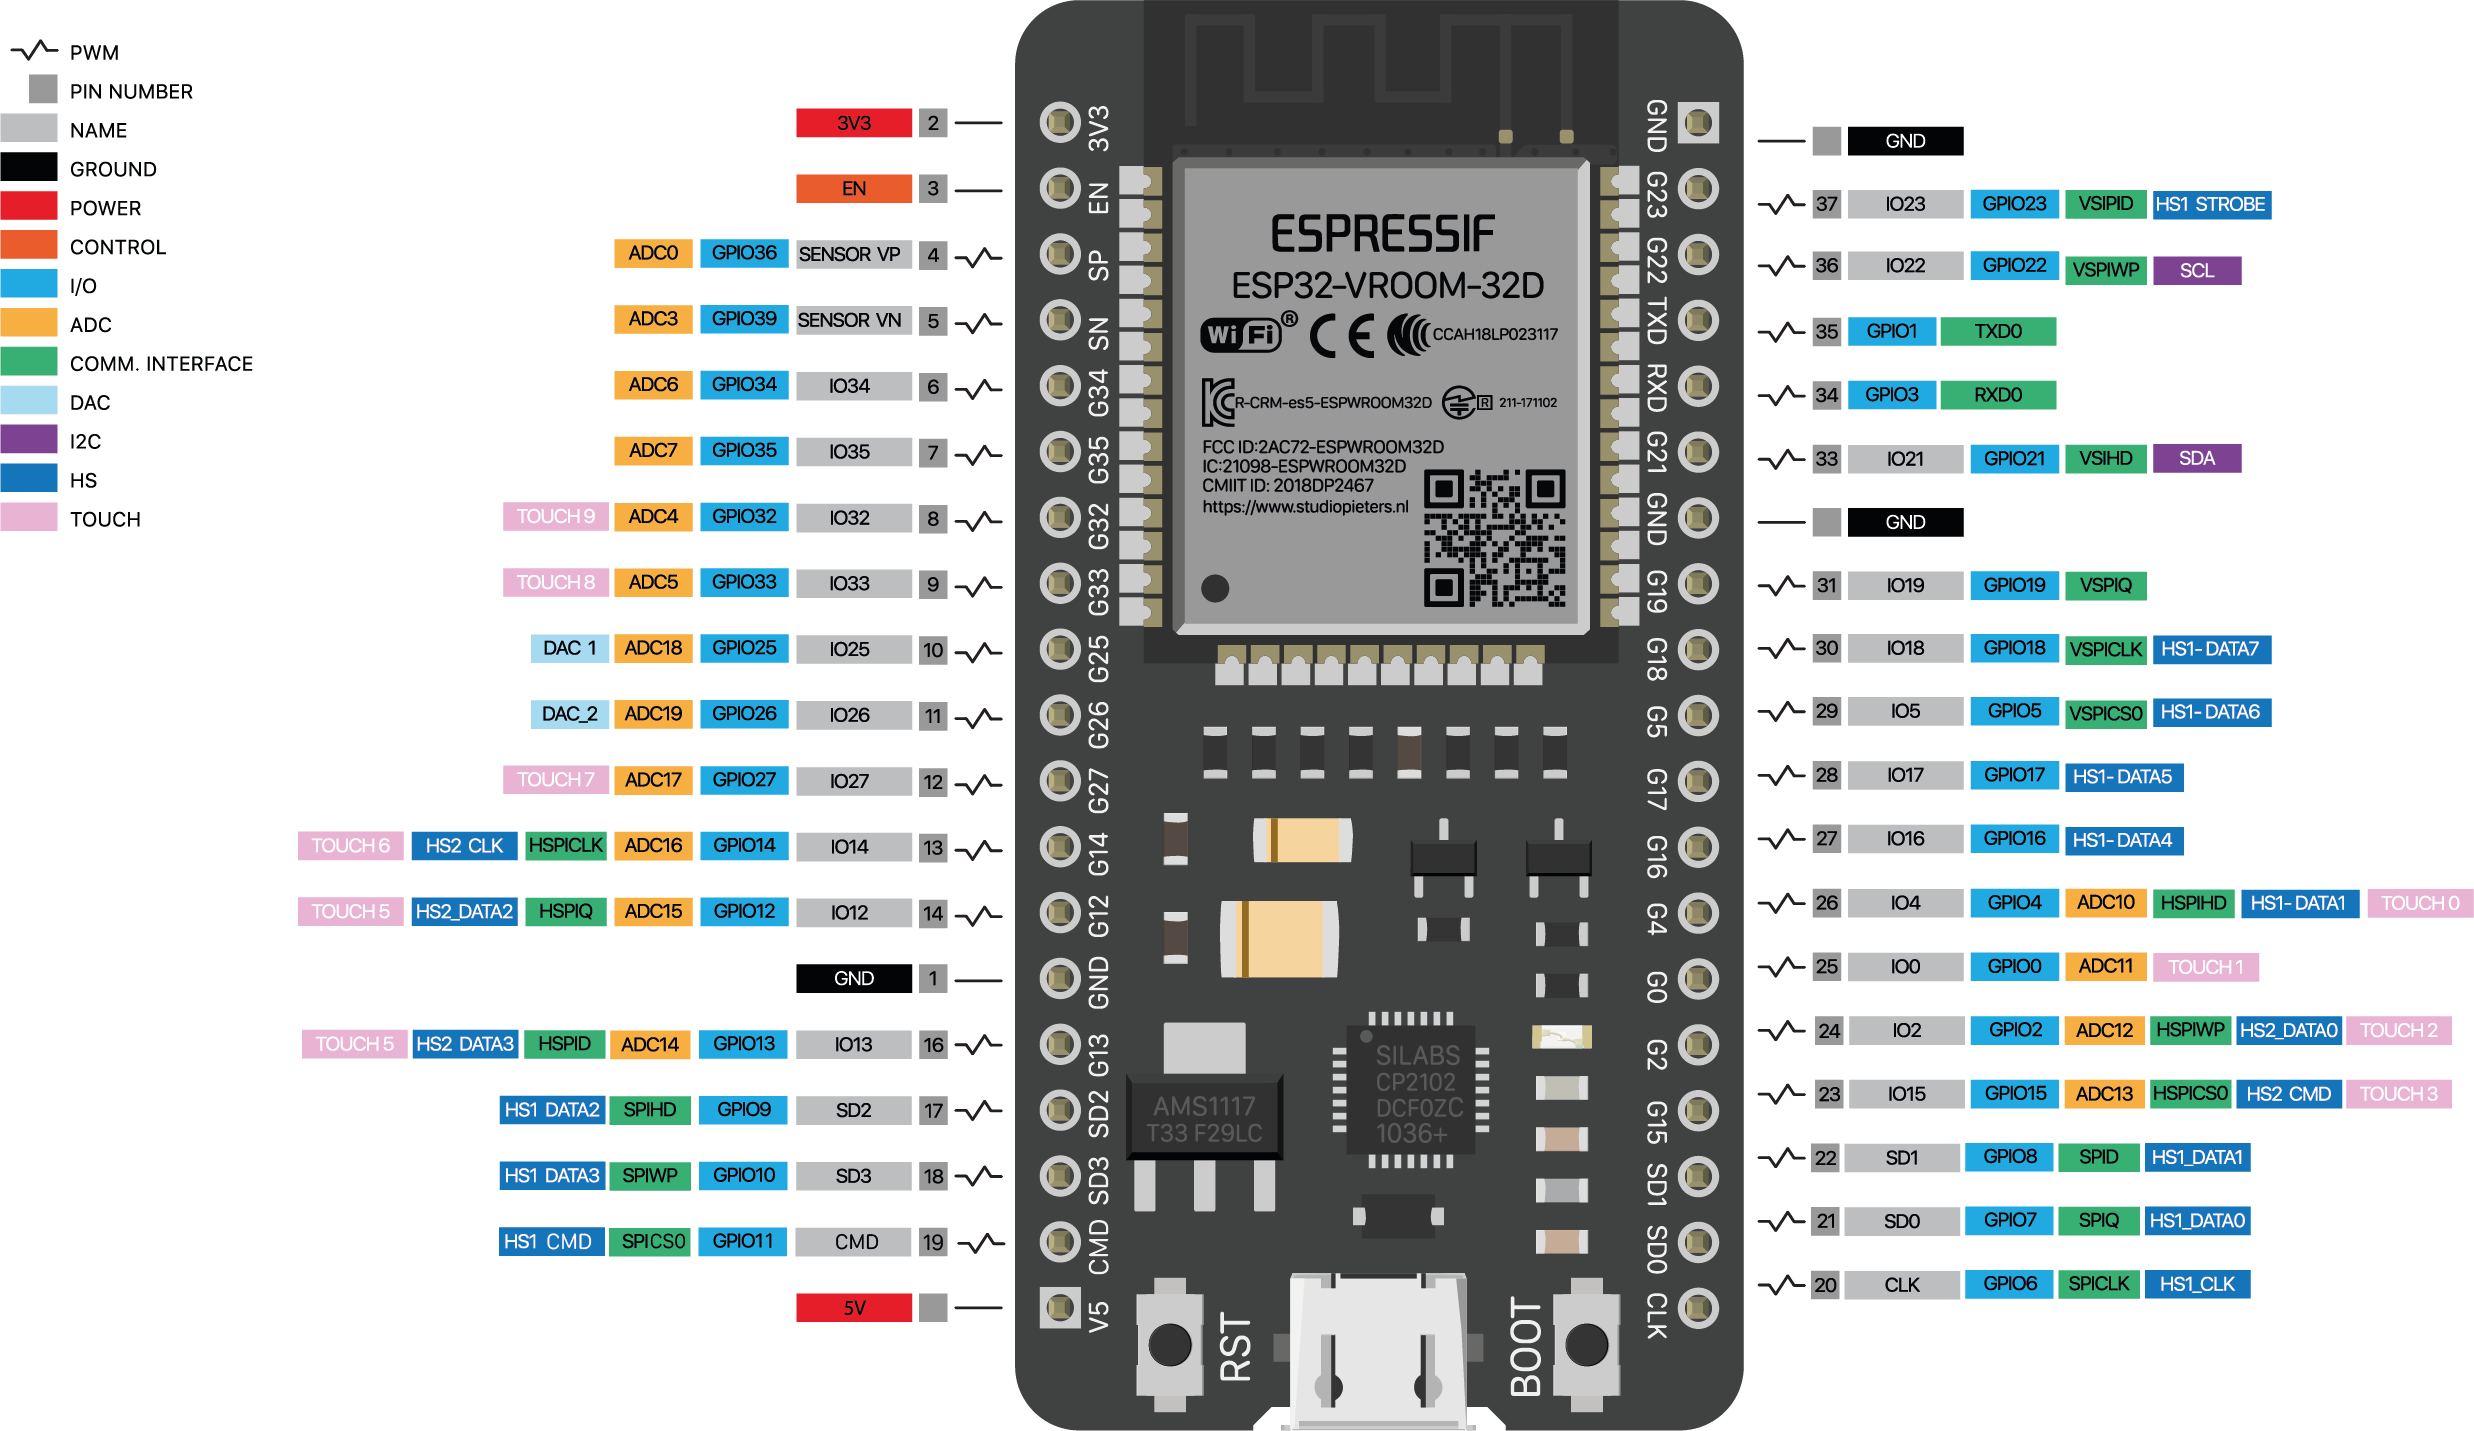
\includegraphics[width=0.5\textwidth]{imagenes/esp32.png}
	\caption{ESP32 pin layout\cite{esp32_img}}
\end{figure}

\section{Micropython}
Micropython \cite{ref12} es una implementación sencilla y eficiente de Python 3 para microcontroladores y otros entornos restringidos. Incluye un pequeño subconjunto de la biblioteca estándar de Python, y se puede extender fácilmente con módulos escritos en C. Micropython es un lenguaje de programación de alto nivel, por lo que es muy sencillo de programar. El firmware de Micropython es muy ligero, por lo que tan solo necesitamos 256Kb de memoria flash y 16Kb de RAM para poder ejecutarlo. \\

Ejemplo de como cambiar el valor de un pin digital\cite{ref13}:
\begin{lstlisting}[language=Python]
from machine import Pin

p0 = Pin(0, Pin.OUT)    # create output pin on GPIO0
p0.on()                 # set pin to "on" (high) level
p0.off()                # set pin to "off" (low) level
p0.value(1)             # set pin to on/high

p2 = Pin(2, Pin.IN)     # create input pin on GPIO2
print(p2.value())       # get value, 0 or 1

p4 = Pin(4, Pin.IN, Pin.PULL_UP) # enable internal pull-up resistor
p5 = Pin(5, Pin.OUT, value=1) # set pin high on creation
p6 = Pin(6, Pin.OUT, drive=Pin.DRIVE_3) # set maximum drive strength

\end{lstlisting}
\section{Comunicaciones inalámbricas en IoT}
Uno de los objetivos principales de este proyecto es poder enviar los datos que recoge cada sensor de corriente a un servidor para que se puedan procesar, analizar y mostrar en conjunto. Para ello, necesitamos alguna forma de comunicación inalámbrica. \\
\subsection{MQTT}
MQTT (Message Queuing Telemetry Transport) \cite{ref14} es un protocolo de mensajería ligero que se utiliza para la comunicación entre dispositivos en IoT. MQTT es un protocolo de publicación/ suscripción, por lo que los dispositivos se suscriben a un topic y los mensajes se publican en ese topic. \\

Caracteristicas principales:
\begin{itemize}
	\item Ligero y eficiente. Los clientes necesitas pocos recursos para poder usar el protocolo, lo que lo hace ideal para usarlo en microcontroladores.
	\item Comunicación bidireccional. Los clientes pueden publicar y suscribirse a topics.
	\item Es un protocolo muy escalable.
	\item Seguridad. MQTT permite el uso de TLS para encriptar la comunicación o el uso de protocolos de autenticación.
	\item Fiabilidad en la entrega de mensajes. MQTT permite especificar el nivel de fiabilidad(Quality of Service) en diferentes niveles. 
\end{itemize}
\begin{figure}[h!]
	\centering
	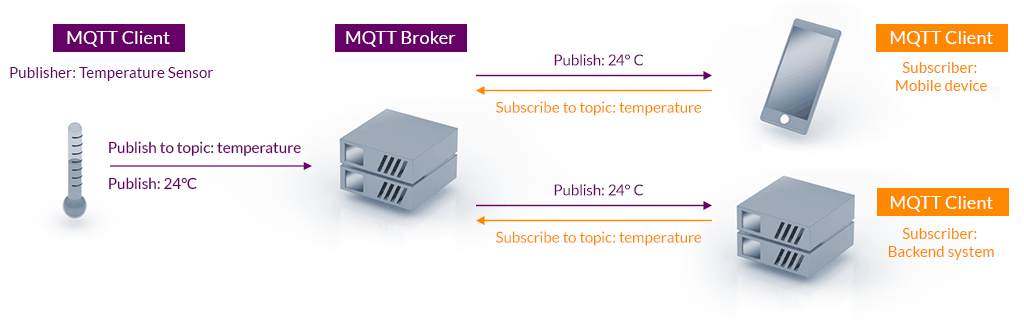
\includegraphics[width=0.75\textwidth]{imagenes/mqtt.png}
	\caption{Ejemplo de dispositivos comunicados por MQTT\cite{mqtt_img}}
\end{figure}

Es importante destacar la importancia del broker en MQTT. El broker es el encargado de recibir los mensajes de los clientes y reenviarlos a los clientes suscritos al topic. \\

\subsection{Zigbee}
Zigbee\cite{ref15} es un estandar de comunicación inalámbrica que se utiliza para la comunicación entre dispositivos en IoT. Zigbee es un protocolo de red mesh, por lo que los dispositivos se comunican entre ellos y no con un broker central a diferencia de MQTT.\\

En Zigbee, podemos encontrar tres clases diferentes de dispositivos:
\begin{itemize}
	\item Zigbee coordinator: El el dispositivo mas capaz encargado de administrar la red y de coordinar la comunicación entre los dispositivos.
	\item Zigbee router: Es un dispositivo que se encarga de reenviar los mensajes de los dispositivos a otros dispositivos ademas de correr su propia aplicación
	\item Zigbee end device: Contiene lo basico para poder comunicarse con un nodo padre y correr su propia aplicación.
\end{itemize}
\begin{figure}[h!]
	\centering
	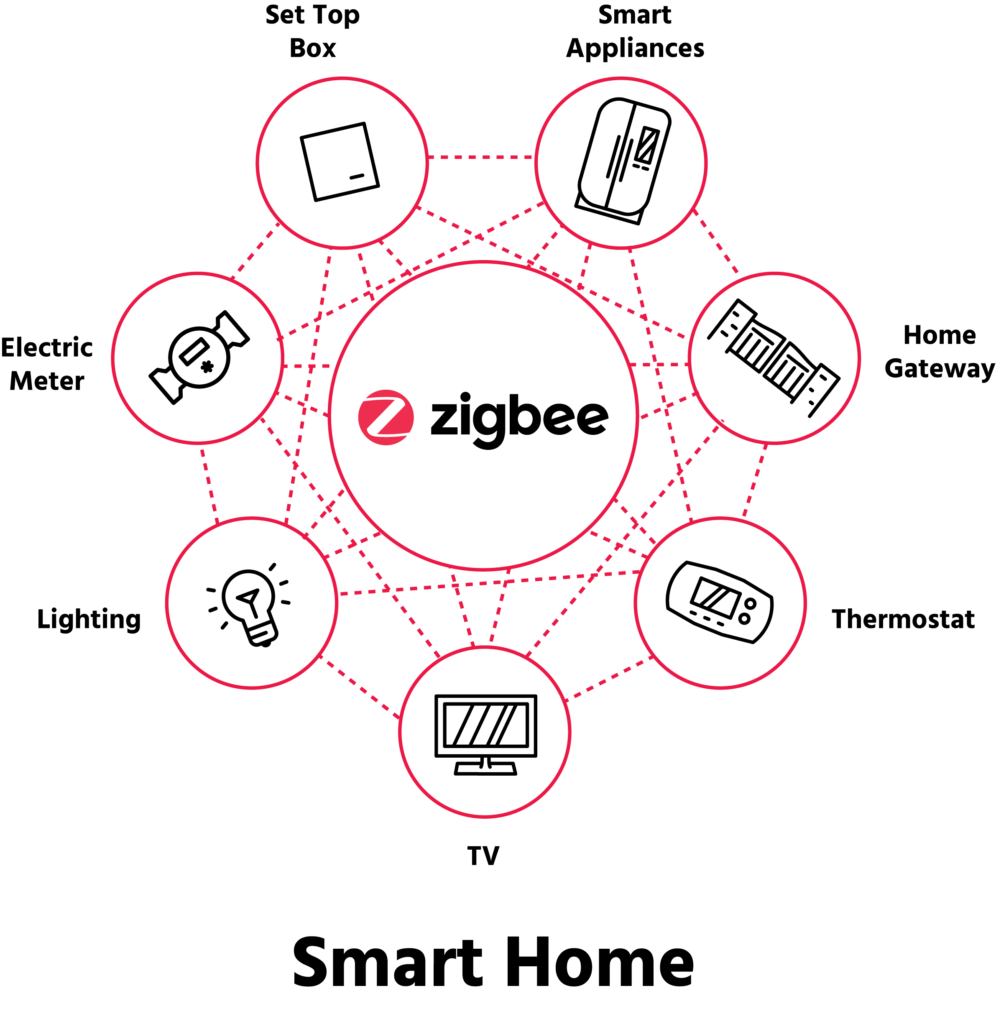
\includegraphics[width=0.45\textwidth]{imagenes/zigbee.png}
	\caption{Ejemplo de dispositivos comunicados por Zigbee\cite{zigbee_img}}
\end{figure}
Caracteristicas principales:
\begin{itemize}
	\item Es un protocolo de red mesh.
	\item Protocolo de bajo consumo, baja latencia y bajo coste.
	\item Es un protocolo de baja potencia, por lo que es ideal para usarlo en dispositivos que necesitan una comunicación a corta distancia.
	\item Hasta 65000 nodos en una red.
	\item Soporta encriptación AES-128.
\end{itemize}
\end{titlepage}
 %Fundamentación teórica y conceptual
%
\begin{titlepage}

\chapter{Implementación del sensor de corriente}
\section{Descripción general}
Para el desarrollo de este proyecto estamos buscando una plataforma de bajo coste que permita comunicación inalámbrica entre dispositivos y que permita el uso de Micropython. Para ello hemos elegido la placa ESP32 de Espressif, que es de bajo coste y tiene un microcontrolador Tensilica LX6 dual con dos núcleos de procesamiento de 32 bits, 512 KB de SRAM y 4 MB de memoria flash. Además, tiene un módulo Wi-Fi y Bluetooth integrado. Se alimenta a 5V y tiene un consumo\cite{ref16} de entre 160mA y 260mA con el WiFi activo. \\

Como sensor de corriente se va a utilizar el ACS712 de 5A y 30A para poder realizar diferentes mediciones y poder comparar los resultados. \\

Como broker MQTT se va a utilizar Mosquitto, que es un broker de código abierto que se puede instalar en cualquier sistema operativo. En este caso, en una Raspberry Pi 2B con Raspbian.\\


\section{Setup experimental}
Lo primero a tener en cuenta es que el sensor ACS712 necesita una tensión de alimentación de 5V y una corriente de 20mA. El pin de salida del sensor es un pin analógico que da una tensión entre 0 y 5V. Si conectaramos este pin directamente a un ADC del ESP32, podriamos llegar a dañar la placa puesto que los ADCs del ESP32 estan diseñados para trabajar con hasta un máximo de 3.3V (a nivel practica es un poco mas de 3.3V). Para evitar esto, se tiene que utilizar un divisor de voltaje que reduzca la tensión de salida del sensor a un valor que pueda leer el ADC. Para ello se ha utilizado una resistencia de 10k y otro de 20k para que el voltaje máximo de salida del sensor sea de 3.3V.\\
\begin{figure}[h!]
	\centering
	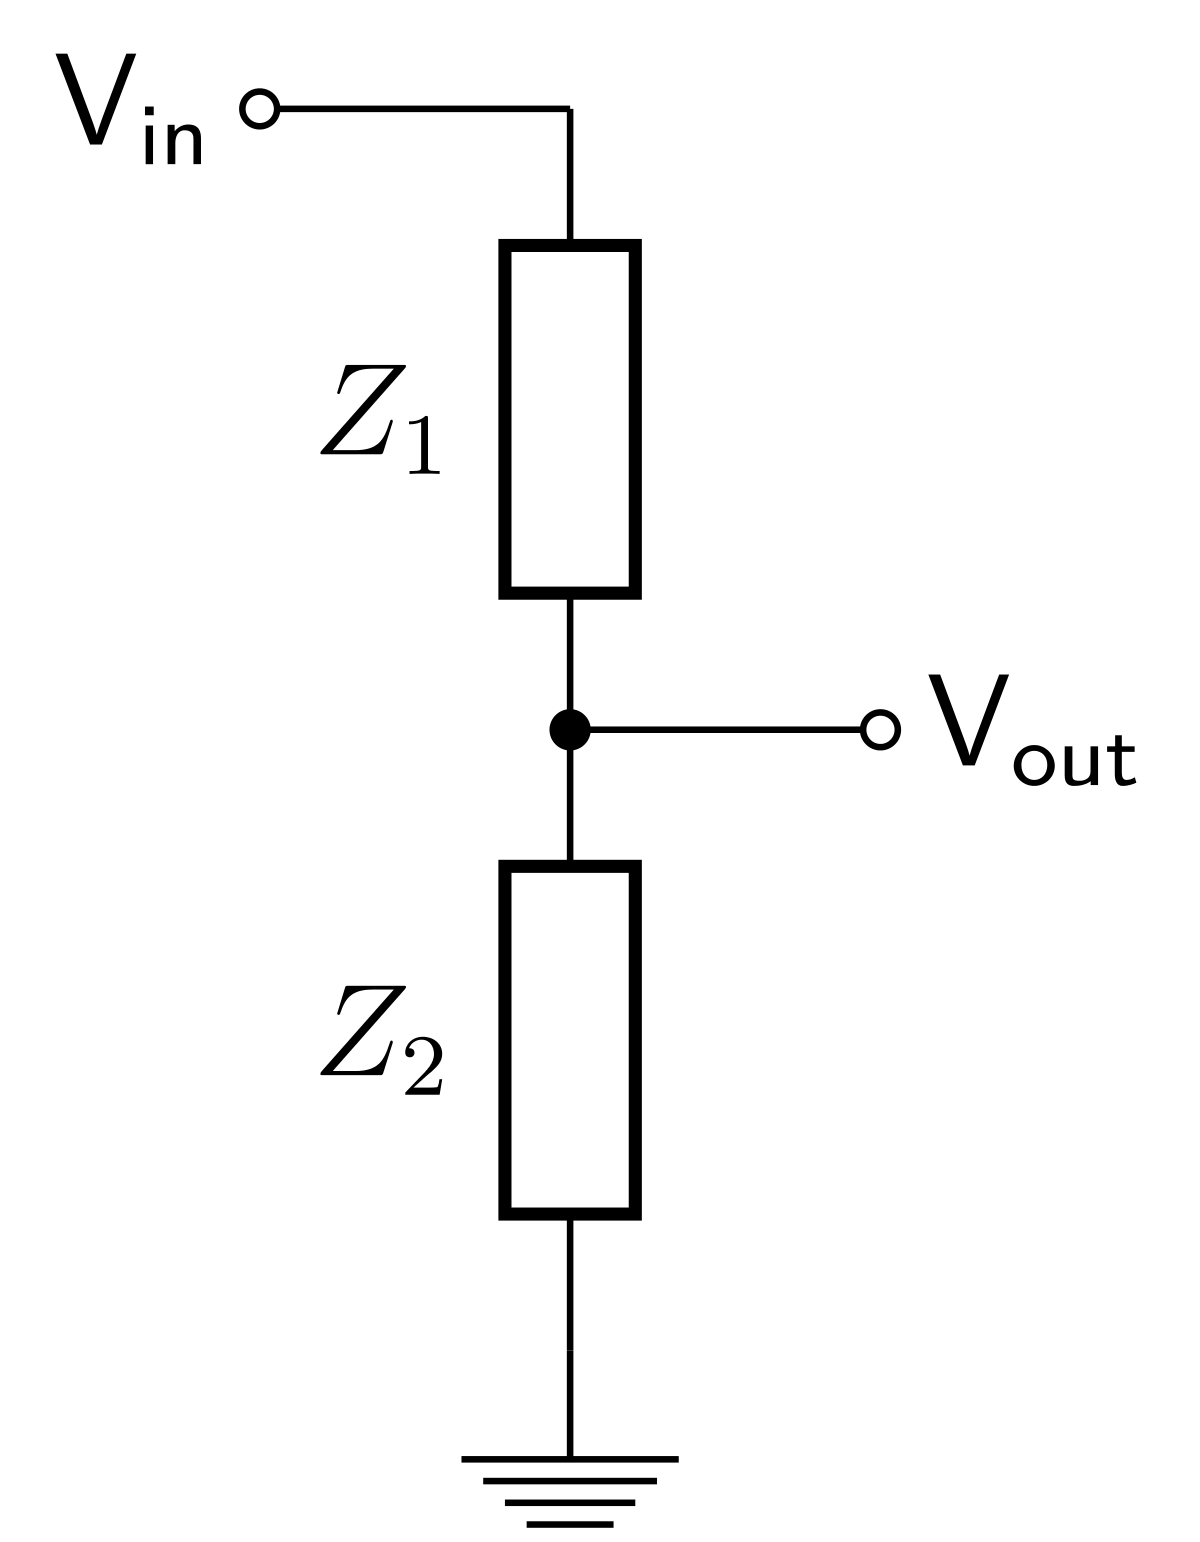
\includegraphics[width=0.20\textwidth]{imagenes/voltage_divider.png}
	\caption{Divisor de voltaje\cite{voltage_divider_img}}
\end{figure}

El segundo componente a añadir es un filtro pasabajos para eliminar el ruido de la señal. Para ello se ha utilizado un capacitor de 100nF conectado entre el pin de salida del sensor y ground para que la señal pase por el capacitor y se elimine el ruido.\\

Lo siguiente es tener una pantalla LED o LCD para poder mostrar por ahi los datos que se van midiendo del sensor de corriente. Para ello se ha utilizado el modulo SSD1306 de 128x32 pixeles. Este modulo se comunica con el ESP32 mediante el protocolo I2C. Para poder comunicar el ESP32 con el modulo SSD1306 se ha utilizado la libreria de Adafruit para el ESP32 en Micropython.\\

Por último, queremos disponer de un boton de reset en el ESP32 en caso de que la configuración que guardemos del servidor MQTT cambie y queramos reiniciar la configuración interna. El ESP32 tiene dos botones que vienen en la placa, pero ninguno de ellos se puede cambiar su función por software, por lo que debemos añadir un boton externo conectado a un pin del ESP32. \\

\begin{figure}[h!]
	\centering
	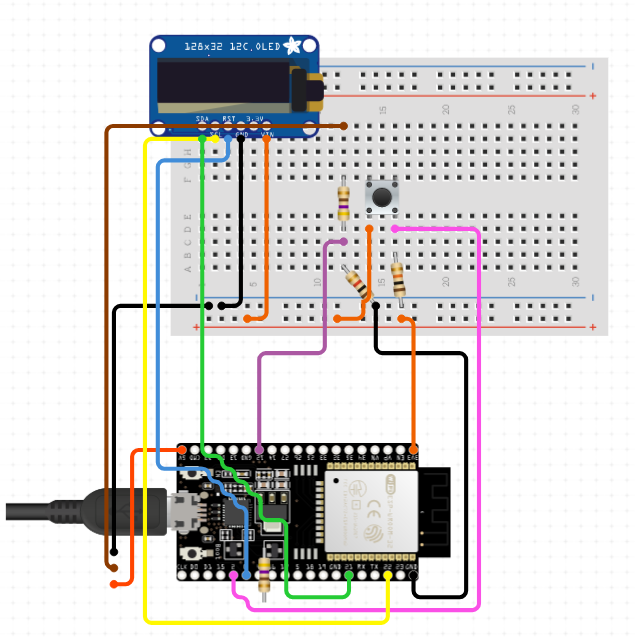
\includegraphics[width=0.75\textwidth]{imagenes/setup.png}
	\caption{Setup experimental}
\end{figure}
\subsection{Preparar ESP32 para Micropython}
Antes de poder usar el ESP32 para ejecutar python, debemos de grabar el firmware correspondiente a la placa. El proceso es bastante sencillo utilizando la herramienta Esptool\cite{ref17}:
\begin{itemize}
	\item En lugar de instalar la herramienta usando pip de python, recomiendo descargar el codigo fuente desde la pagina de github\cite{ref18} y ejecutar el archivo esptool.py directamente ya que al menos en mi experiencia da menos problemas.
	\item Una vez con la herramienta instalada, lo primero es borrar completamente la memoria flash de la placa. Ejecutaremos el siguiente comando(en mi caso, ttyUSB0 para indicar el puerto al que esta conectado):
\end{itemize}
\begin{lstlisting}[language=Bash]
	esptool.py --port /dev/ttyUSB0 erase_flash
\end{lstlisting}
\begin{itemize}
	\item Ahora, debemos de grabar el firmware de Micropython en la placa. Para ello, descargaremos el firmware (.bin) de la pagina oficial\cite{ref19} y ejecutaremos el siguiente comando:
\end{itemize}
\begin{lstlisting}[language=python]
	esptool.py --port /dev/ttyUSB0 write_flash -z 0x1000 esp32.bin
\end{lstlisting}
\begin{itemize}
	\item Si todo ha ido bien, ya podremos ejecutar Micropython en la placa. Podemos comprobarlo conectandonos por el puerto serie a la placa (en el ejemplo uso picocom pero se puede utilizar cualquier software que permita la conexion por serial) y viendo si la placa nos responde con el prompt de Micropython:
\end{itemize}
	\begin{lstlisting}
		$ picocom /dev/ttyUSB0 -b115200
	\end{lstlisting}
	\begin{figure}[h!]
		\centering
		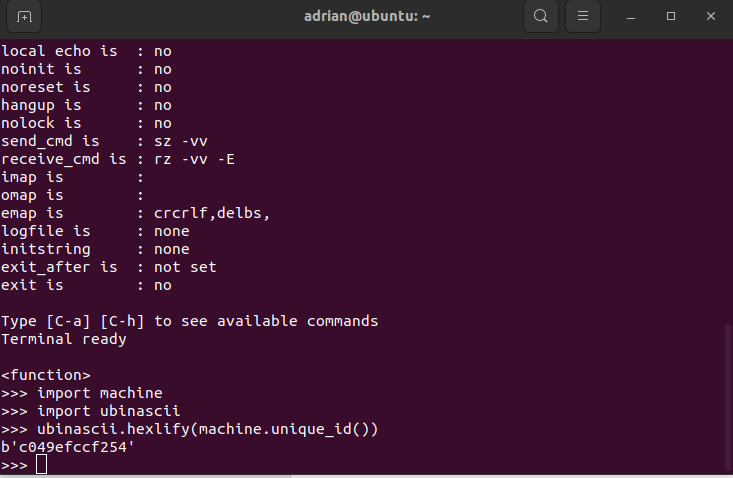
\includegraphics[width=0.75\textwidth]{imagenes/micropython_prompt.png}
		\caption{Prompt de Micropython}
	\end{figure}

\subsection{Micropython en ESP32}
Despues de instalar el firmware de Micropython en la placa, podremos observar que hay un archivo llamado boot.py que se ejecuta al arrancar la placa. En este archivo se puede configurar la placa para que se conecte a una red WiFi o para que se conecte a un servidor MQTT.\\
Despues de este boot.py, la placa intentará ejecutar el archivo main.py si existe. En este archivo se puede programar el comportamiento de la placa.\\

Al igual que en python, podemos hacer uso de diferentes librerias. Para poder usar librerias que no vengan por defecto en el firmware de Micropython, debemos de copiar los archivos .py a la flash de la placa con la herramienta Ampy de Adafruit\cite{ref20}. Con Ampy podemos desde copiar un archivo a la flash de la placa o recuperar un archivo de la flash de la placa a nuestro ordenador. \\
Uso de Ampy:
\begin{figure}[h!]
	\centering
	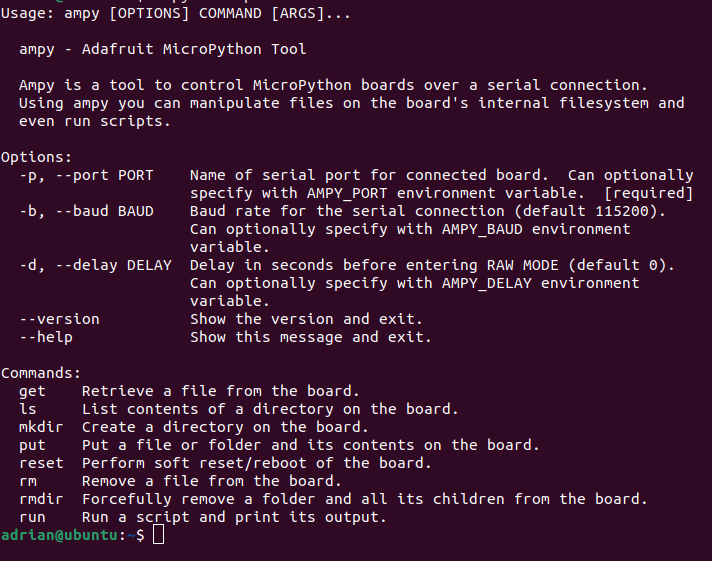
\includegraphics[width=0.75\textwidth]{imagenes/ampy.png}
	\caption{Opciones de Ampy}
\end{figure}
\subsection{Librerias utilizadas}
\subsubsection{Libreria para el SSD1306}
Para usar el modulo SSD1306, se ha utilizado la libreria \cite{ref21} en Micropython. Esta libreria nos permite inicializar el modulo SSD1306 y escribir texto en la pantalla de manera sencilla.\\
\subsubsection{Libreria para MQTT}
Para usar MQTT, se ha utilizado la libreria umqtt.simple\cite{ref22} en Micropython. Esta libreria nos permite conectarnos a un servidor MQTT y publicar y subscribirse a diferentes topics.\\
\newpage
\section{Implementación}
\subsection{Diagrama de estados}
\subsubsection{Init}
La inicialización del programa empieza por conectarse a la red WiFi y al broker de MQTT. A continuación comprobamos si ya hemos establecido conexión previamente con la aplicación web. Si no se ha establecido previamente conexión con la aplicación web, empezaremos a publicar periodicamente el ID interno del ESP32 y esperaremos a que la aplicaciób web nos devuelva el ACK. Lo siguiente es comprobar si hemos recibido la configuración de la aplicación web (la configuración a recibir es el tipo de sensor y el voltaje al que estamos conectados). Por último calibramos el sensor, es decir, leemos el voltaje de salida del ACS712 durante un periodo de tiempo sin que haya nada conectado al sensor y lo guardamos como voltaje de referencia para poder calcular la corriente en el futuro.\\
\begin{figure}[h!]
	\centering
	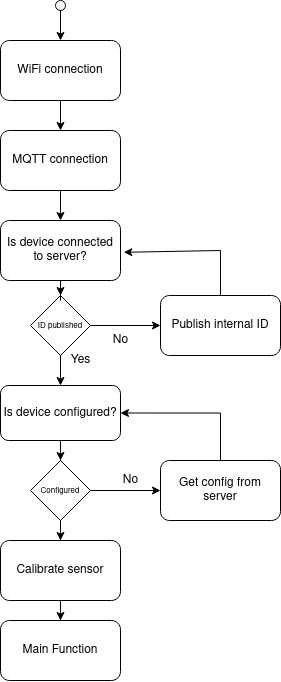
\includegraphics[width=0.30\textwidth]{imagenes/Init.drawio.png}
	\caption{Diagrama de estados Init}
\end{figure}
\subsubsection{Main}
La función principal es bastante sencilla. En cada iteración, lanzamos una llamada a la libreria de MQTT para comprobar si hay mensajes en la cola recibidos (esto hará que se lance el callback de recepción de mensajes MQTT si es que hay alguno). Lo siguiente es leer el voltaje de salida del sensor de corriente y calcular el amperaje y consumo (en Watts). Estos watios calculados los mostramos por el dispositivo OLED que tenemos conectado. Por último, publicamos el valor del amperaje y consumo en el topic de MQTT correspondiente (watts/ID\_Sensor y amps/ID\_Sensor)

\begin{figure}[h!]
	\centering
	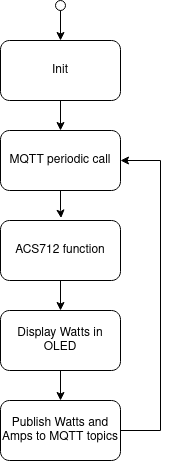
\includegraphics[width=0.30\textwidth]{imagenes/main.drawio.png}
	\caption{Diagrama de estados función Main}
\end{figure}
\newpage
\subsubsection{Lectura del sensor}
\begin{figure}[h!]
	\centering
	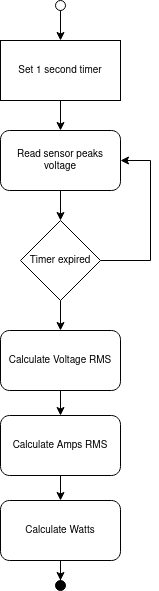
\includegraphics[width=0.30\textwidth]{imagenes/acs712.drawio.png}
	\caption{Diagrama de la función de lectura del ACS712}
\end{figure}

\subsection{Código}
\subsubsection{Función Init}
\begin{lstlisting}[language=python]
display_message('Connecting to WiFi...')
connect_wifi(SSID, PASSWORD)

#display_message('Connecting to MQTT broker...')
MQTT_CLIENT.connect()
MQTT_CLIENT.mqtt.set_callback(subscribe_callback)
if MQTT_CLIENT.is_broker_acknowledged() == False:
	MQTT_CLIENT.publish_clientID()

#subscribe to reset topic
MQTT_CLIENT.subscribe('reset/' + MQTT_CLIENT.client_id.decode("utf-8"))
#subscribe to sensor_config topic to receive the sensor voltage
MQTT_CLIENT.subscribe('sensor_config/' + MQTT_CLIENT.client_id.decode("utf-8"))

display_message('Configuring sensor...')
if CURRENT_SENSOR.is_sensor_configured() == False:
	MQTT_CLIENT.get_sensor_config_from_broker()

#subscribe to restart esp32 topic
MQTT_CLIENT.subscribe('restart/' + MQTT_CLIENT.client_id.decode("utf-8"))

display_message('Calibrating...')
CURRENT_SENSOR.calibrateSensorAC()

#subscribe to calibrate topic
MQTT_CLIENT.subscribe('calibrate/' + MQTT_CLIENT.client_id.decode("utf-8"))
\end{lstlisting}

\subsubsection{Función de calibración del sensor}
\begin{lstlisting}[language=python]
def calibrateSensorAC(self, seconds=10):
	"""
	Calibrate the sensor to get the average voltage 
	reading when there is no load.
	"""
	print("[testCalibrateSensor]Calibrating sensor...")
	print("[testCalibrateSensor]Please disconnect the sensor \
		from the load NOW!")
	for i in reversed(range(5)):
		print("[testCalibrateSensor]Starting calibration in " + 
			str(i+1) + " seconds...")
		utime.sleep(0.5)
	print("[testCalibrateSensor]Calibrating...")
	counter = 0
	voltage_RMS = 0
	average_voltage = 0
	start = time.ticks_ms()
	while time.ticks_ms() - start < (1000 * seconds):
		min_value = 4095
		max_value = 0
		voltage = 0
		for i in range(100):
			adc_raw = self.adc.read()
			voltage += adc_raw
			if adc_raw < min_value:
				min_value = adc_raw
			elif adc_raw > max_value:
				max_value = adc_raw
			time.sleep_us(500)
		average_voltage += ((voltage * 3.3) / 4095) / 100
		counter = counter + 1
		max_value_V = ((max_value * 3.3) / 4095)
		min_value_V = ((min_value * 3.3) / 4095)
		peak_to_peak = (max_value_V - min_value_V)
		voltage_RMS += peak_to_peak * 0.3536
	end = time.ticks_ms()
	print("[readAmps2]Time to read ", counter, " values: ", 
		time.ticks_diff(end, start), "ms")
	voltage_RMS = voltage_RMS / counter
	if voltage_RMS > 0.020:
		self.default_VRMS = voltage_RMS
	else:
		self.default_VRMS = 0.020
	self.default_output_voltage = average_voltage / counter
	#add 5mV to the default output voltage to avoid negative values
	self.default_VRMS = self.default_VRMS + 0.005
	print("[calibrateSensorAC]Sensor calibrated. Default output \
			voltage: ", self.default_output_voltage, "V")
	print("[calibrateSensorAC]Sensor calibrated. Default VRMS: ", 
			self.default_VRMS, "V")
\end{lstlisting}

\subsubsection{Función Main}
\begin{lstlisting}[language=python]
init()

while True:
	MQTT_CLIENT.check_msg()
	watts, amps = CURRENT_SENSOR.getACWatts(logging=False)
	display_watts(watts)
	MQTT_CLIENT.publish('amps/' + 
		MQTT_CLIENT.client_id.decode("utf-8"), str(amps))
	MQTT_CLIENT.publish('watts/' + 
		MQTT_CLIENT.client_id.decode("utf-8"), str(watts))
	print('-----------------------')
\end{lstlisting}

\subsubsection{Funciones de lectura del sensor}
\begin{lstlisting}[language=python]
def readSensorVPP(self, logging=False):
	"""
	Capture the peak to peak voltage of the current ADC signal.
	Period of measurement is 50ms. The ADC is sampled every 500us. 
	100 samples are taken. AC current in spain is 50Hz.
	We should be able to capture at least 2 full cycles of the 
	sinusoidal signal with its peaks.
	"""
	min_value = 4095
	max_value = 0
	average_value = 0
	start = time.ticks_ms()
	for i in range(100):
		adc_raw = self.adc.read()
		average_value += adc_raw
		if adc_raw < min_value:
			min_value = adc_raw
		elif adc_raw > max_value:
			max_value = adc_raw
		time.sleep_us(500)
	end = time.ticks_ms()
	max_value_V = ((max_value * 3.3) / 4095)
	min_value_V = ((min_value * 3.3) / 4095)
	average_value_V = ((average_value / 100) * 3.3) / 4095
	peak_to_peak = (max_value_V - min_value_V)
	if logging:
		print("[readSensorVPP]Time to read 100 samples: ", 
				time.ticks_diff(end, start), "ms")
		print("[readSensorVPP]Average value: ", average_value_V, "V")
		print("[readSensorVPP]Max value: ", max_value_V, "V; Min \
			value: ", min_value_V, "V; VPP: ", peak_to_peak, "V")

	return peak_to_peak, average_value_V 

def readRMSVoltage(self, logging=False):
	voltage_RMS = 0
	voltage_RMS_nofilter = 0
	average_voltage = 0
	samplesVPP = list()
	samplesV = list()
	start = time.ticks_ms()
	while time.ticks_ms() - start < 1000:
		voltagePP, voltage = self.readSensorVPP(logging=False)
		samplesVPP.append(voltagePP * 0.3536)
		samplesV.append(voltage)
	end = time.ticks_ms()
	for i in range(len(samplesVPP)):
		voltage_RMS_nofilter += samplesVPP[i]
		average_voltage += samplesV[i]
	"""
	for sample in samplesVPP:
		voltage_RMS_nofilter += sample
	"""
	voltage_RMS_nofilter = voltage_RMS_nofilter / len(samplesVPP)
	average_voltage = average_voltage / len(samplesV)
	#apply sw filter
	samplesVPP = self.RMSFilter(samplesVPP, logging=False)
	for sample in samplesVPP:
		voltage_RMS += sample
	voltage_RMS = voltage_RMS / len(samplesVPP)

	if logging:
		print("[readRMSVoltage]Time to read ", len(samplesV), 
			" values: ", time.ticks_diff(end, start), "ms")
		print("[readRMSVoltage]Voltage RMS: ", voltage_RMS * 1000, 
			"mV", " default VRMS: ", self.default_VRMS * 1000, "mV")
		print("[readRMSVoltage]Voltage RMS no filter: ", 
			voltage_RMS_nofilter * 1000, "mV", " default VRMS: ", 
				self.default_VRMS * 1000, "mV")
		print("[readRMSVoltage]Average voltage: ", 
			average_voltage * 1000, "mV"," default output voltage: ", 
				self.default_output_voltage * 1000, "mV")
	
	return voltage_RMS, average_voltage

def readRMSAmps(self, logging=False):
	voltage_RMS, voltage = self.readRMSVoltage(logging=logging)
	#decide whether to apply an error correction or not
	if self.checkZeroRange(voltage_RMS, voltage, logging=logging):
		Amps_RMS = 0
	else:
		Amps_RMS = (voltage_RMS * 1000) / self.scale_factor

	amps = abs(((voltage - self.default_output_voltage) * 1000)
		 / self.scale_factor)
	if logging:
		print("[readRMSAmps]Current: ", Amps_RMS, "A RMS")
		print("[readRMSAmps]Current: ", amps, "A")

	return Amps_RMS, amps

def getACWatts(self, logging=False):
	"""
	Calculate the power consumption in Watts.
	"""
	Amps_RMS, amps = self.readRMSAmps(logging=logging)
	if self.type == "AC":
		watts = self.referenceVoltage * Amps_RMS
		ret_amps = Amps_RMS
	elif self.type  == "DC":
		watts = self.referenceVoltage * amps
		ret_amps = amps
	else:
		watts = 0
	if logging:
		print("[getACWatts]Watts: ", watts, "W", "with sensor: ", 
				self.type)

	return watts, ret_amps

\end{lstlisting}

El codigo completo puede ser consultado en el siguiente enlace\cite{ref23}.\\

\section{Test de funcionamiento}
\subsection{Corriente continua}
Para probar diferente amperajes se ha utilizado una fuente de alimentación que permite variar la corriente de salida entre 0 y 3A. La tensión de la fuente se ha fijado en 12V.\\
\subsubsection{No load}
\begin{figure}[h!]
	\centering
	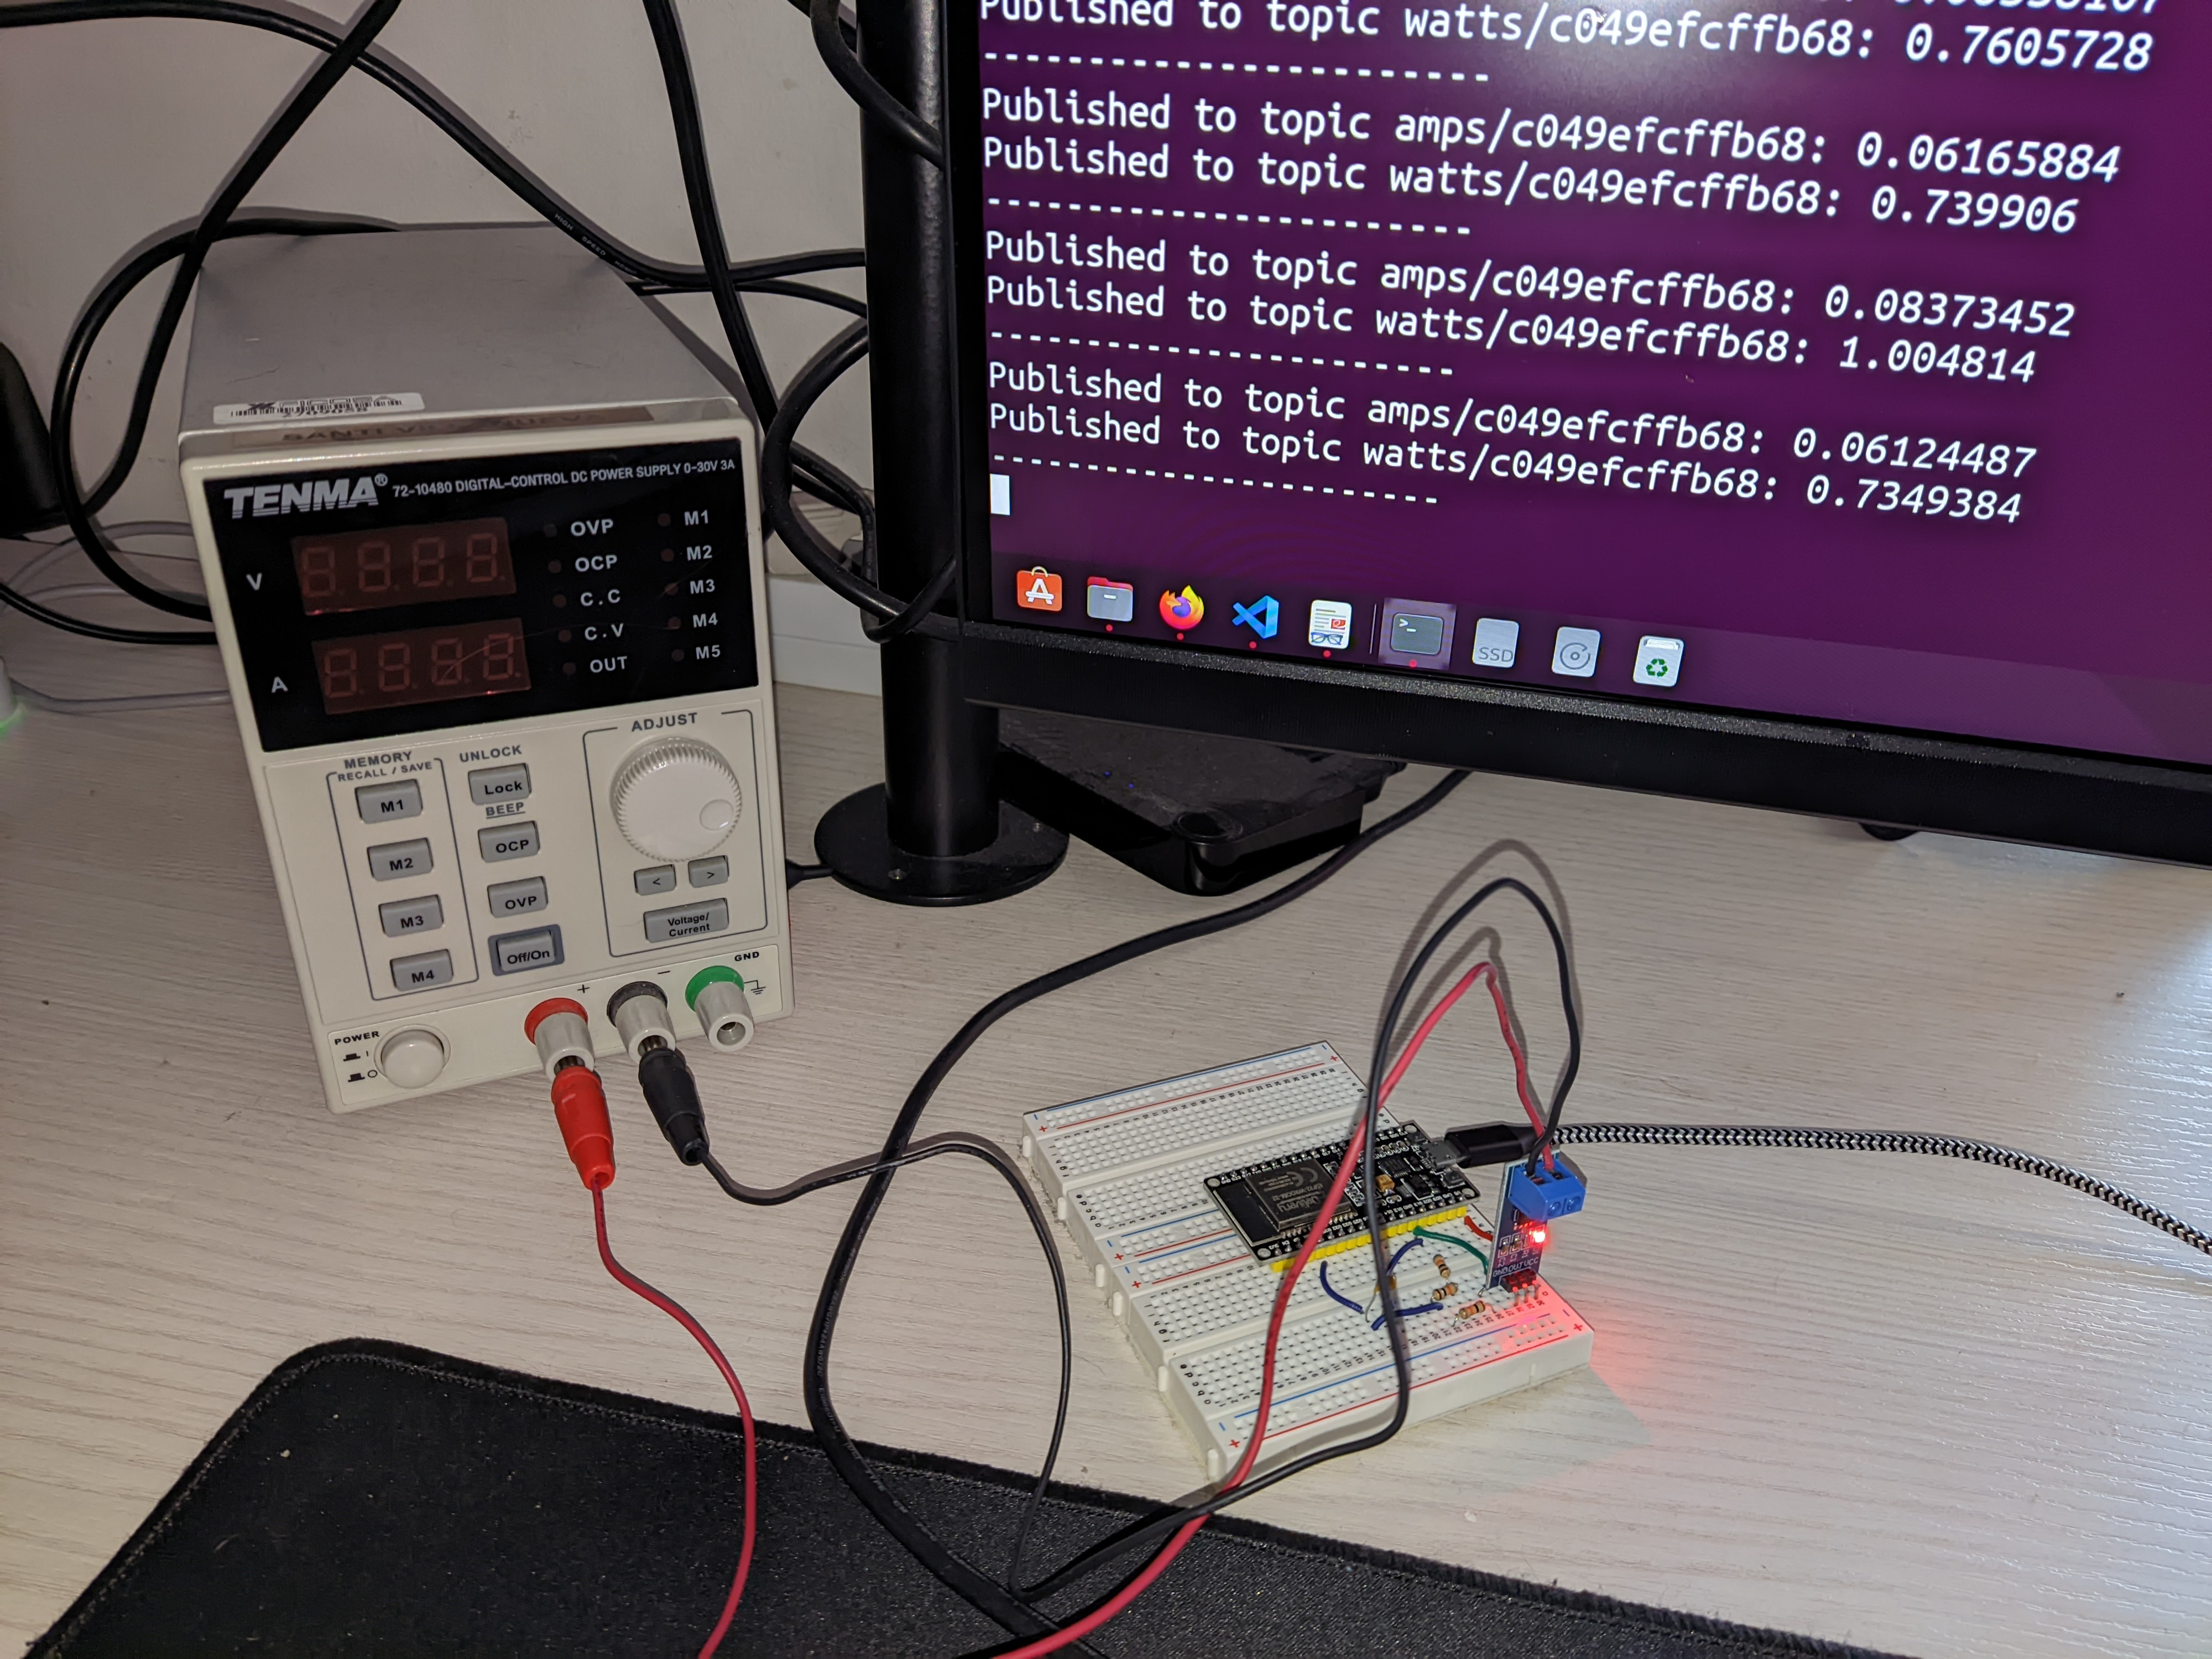
\includegraphics[width=0.5\textwidth]{imagenes/DC_noload.jpg}
	\caption{Salida del ACS712 con corriente continua de 0A}
\end{figure}
Como podemos observar, tras la conversión de la señal del ACS712 a amperios, tenemos valores muy cercanos a 0A que son practicamente despreciables. \\
\subsubsection{1A}
\begin{figure}[h!]
	\centering
	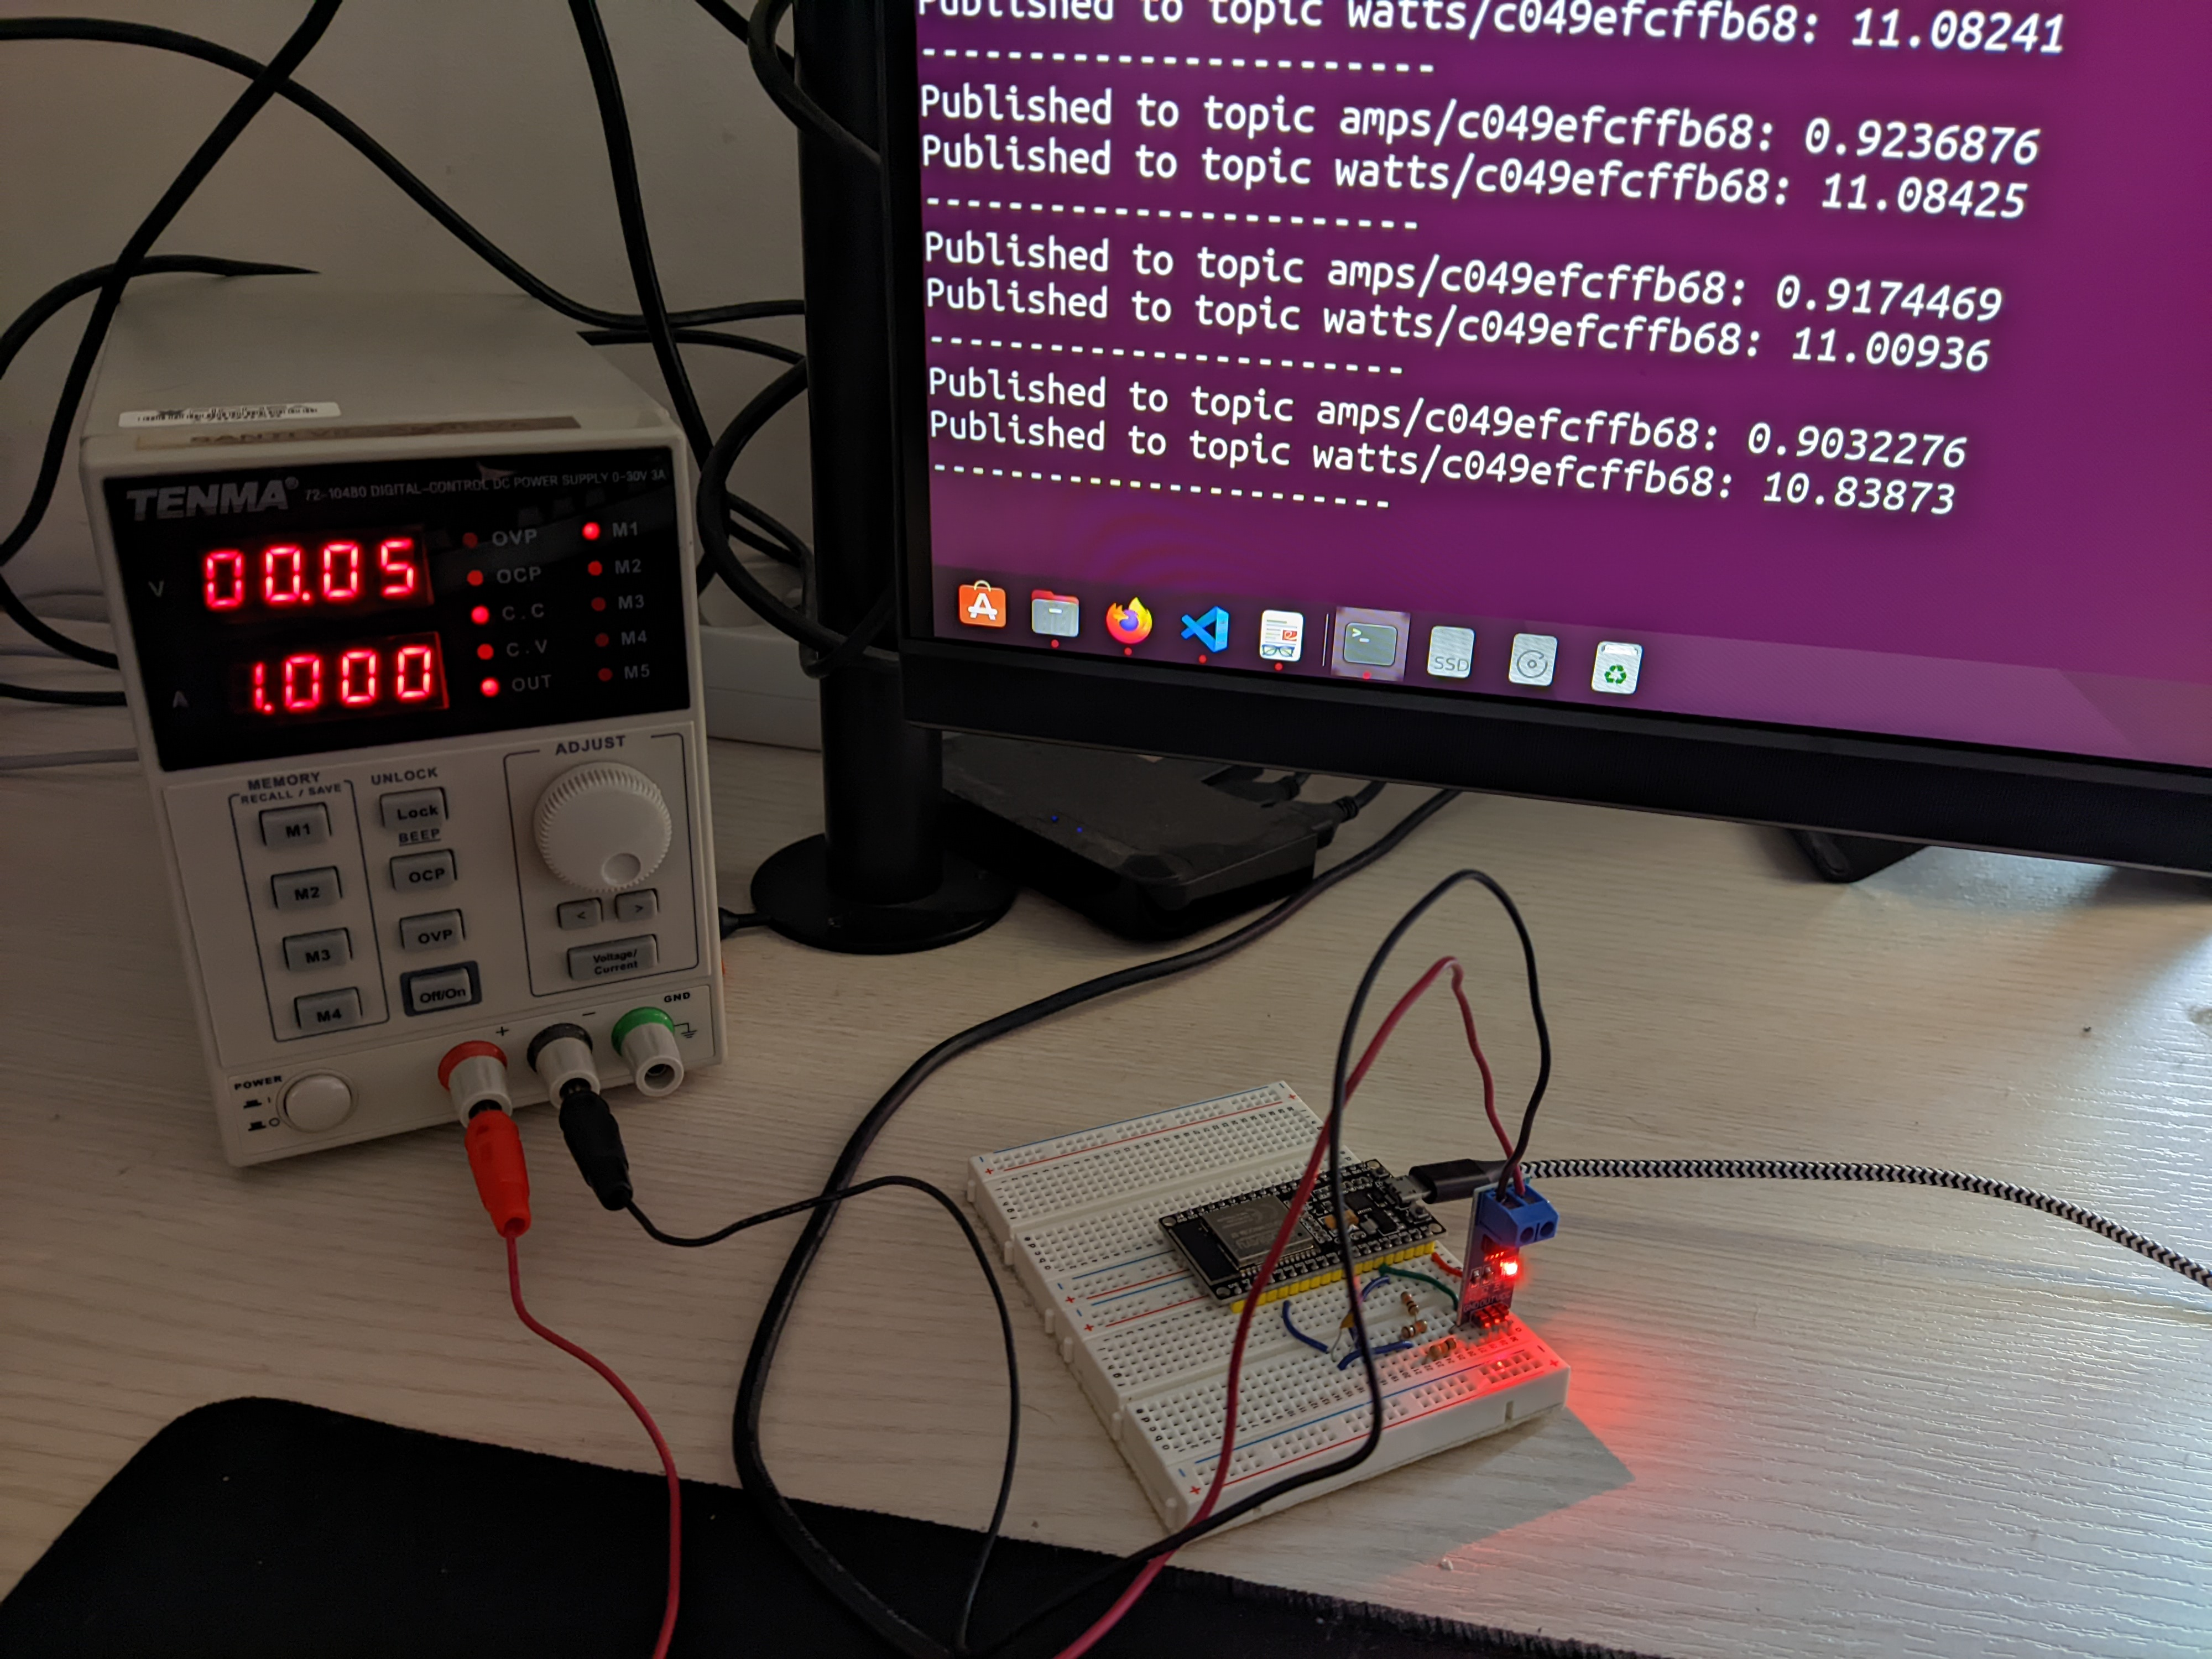
\includegraphics[width=0.5\textwidth]{imagenes/DC_1Amp.jpg}
	\caption{Salida del ACS712 con corriente continua de 1A}
\end{figure}
Generando 1A de corriente continua, medimos 0.91A con el sensor ACS712. \\
\subsubsection{1.7A}
\begin{figure}[h!]
	\centering
	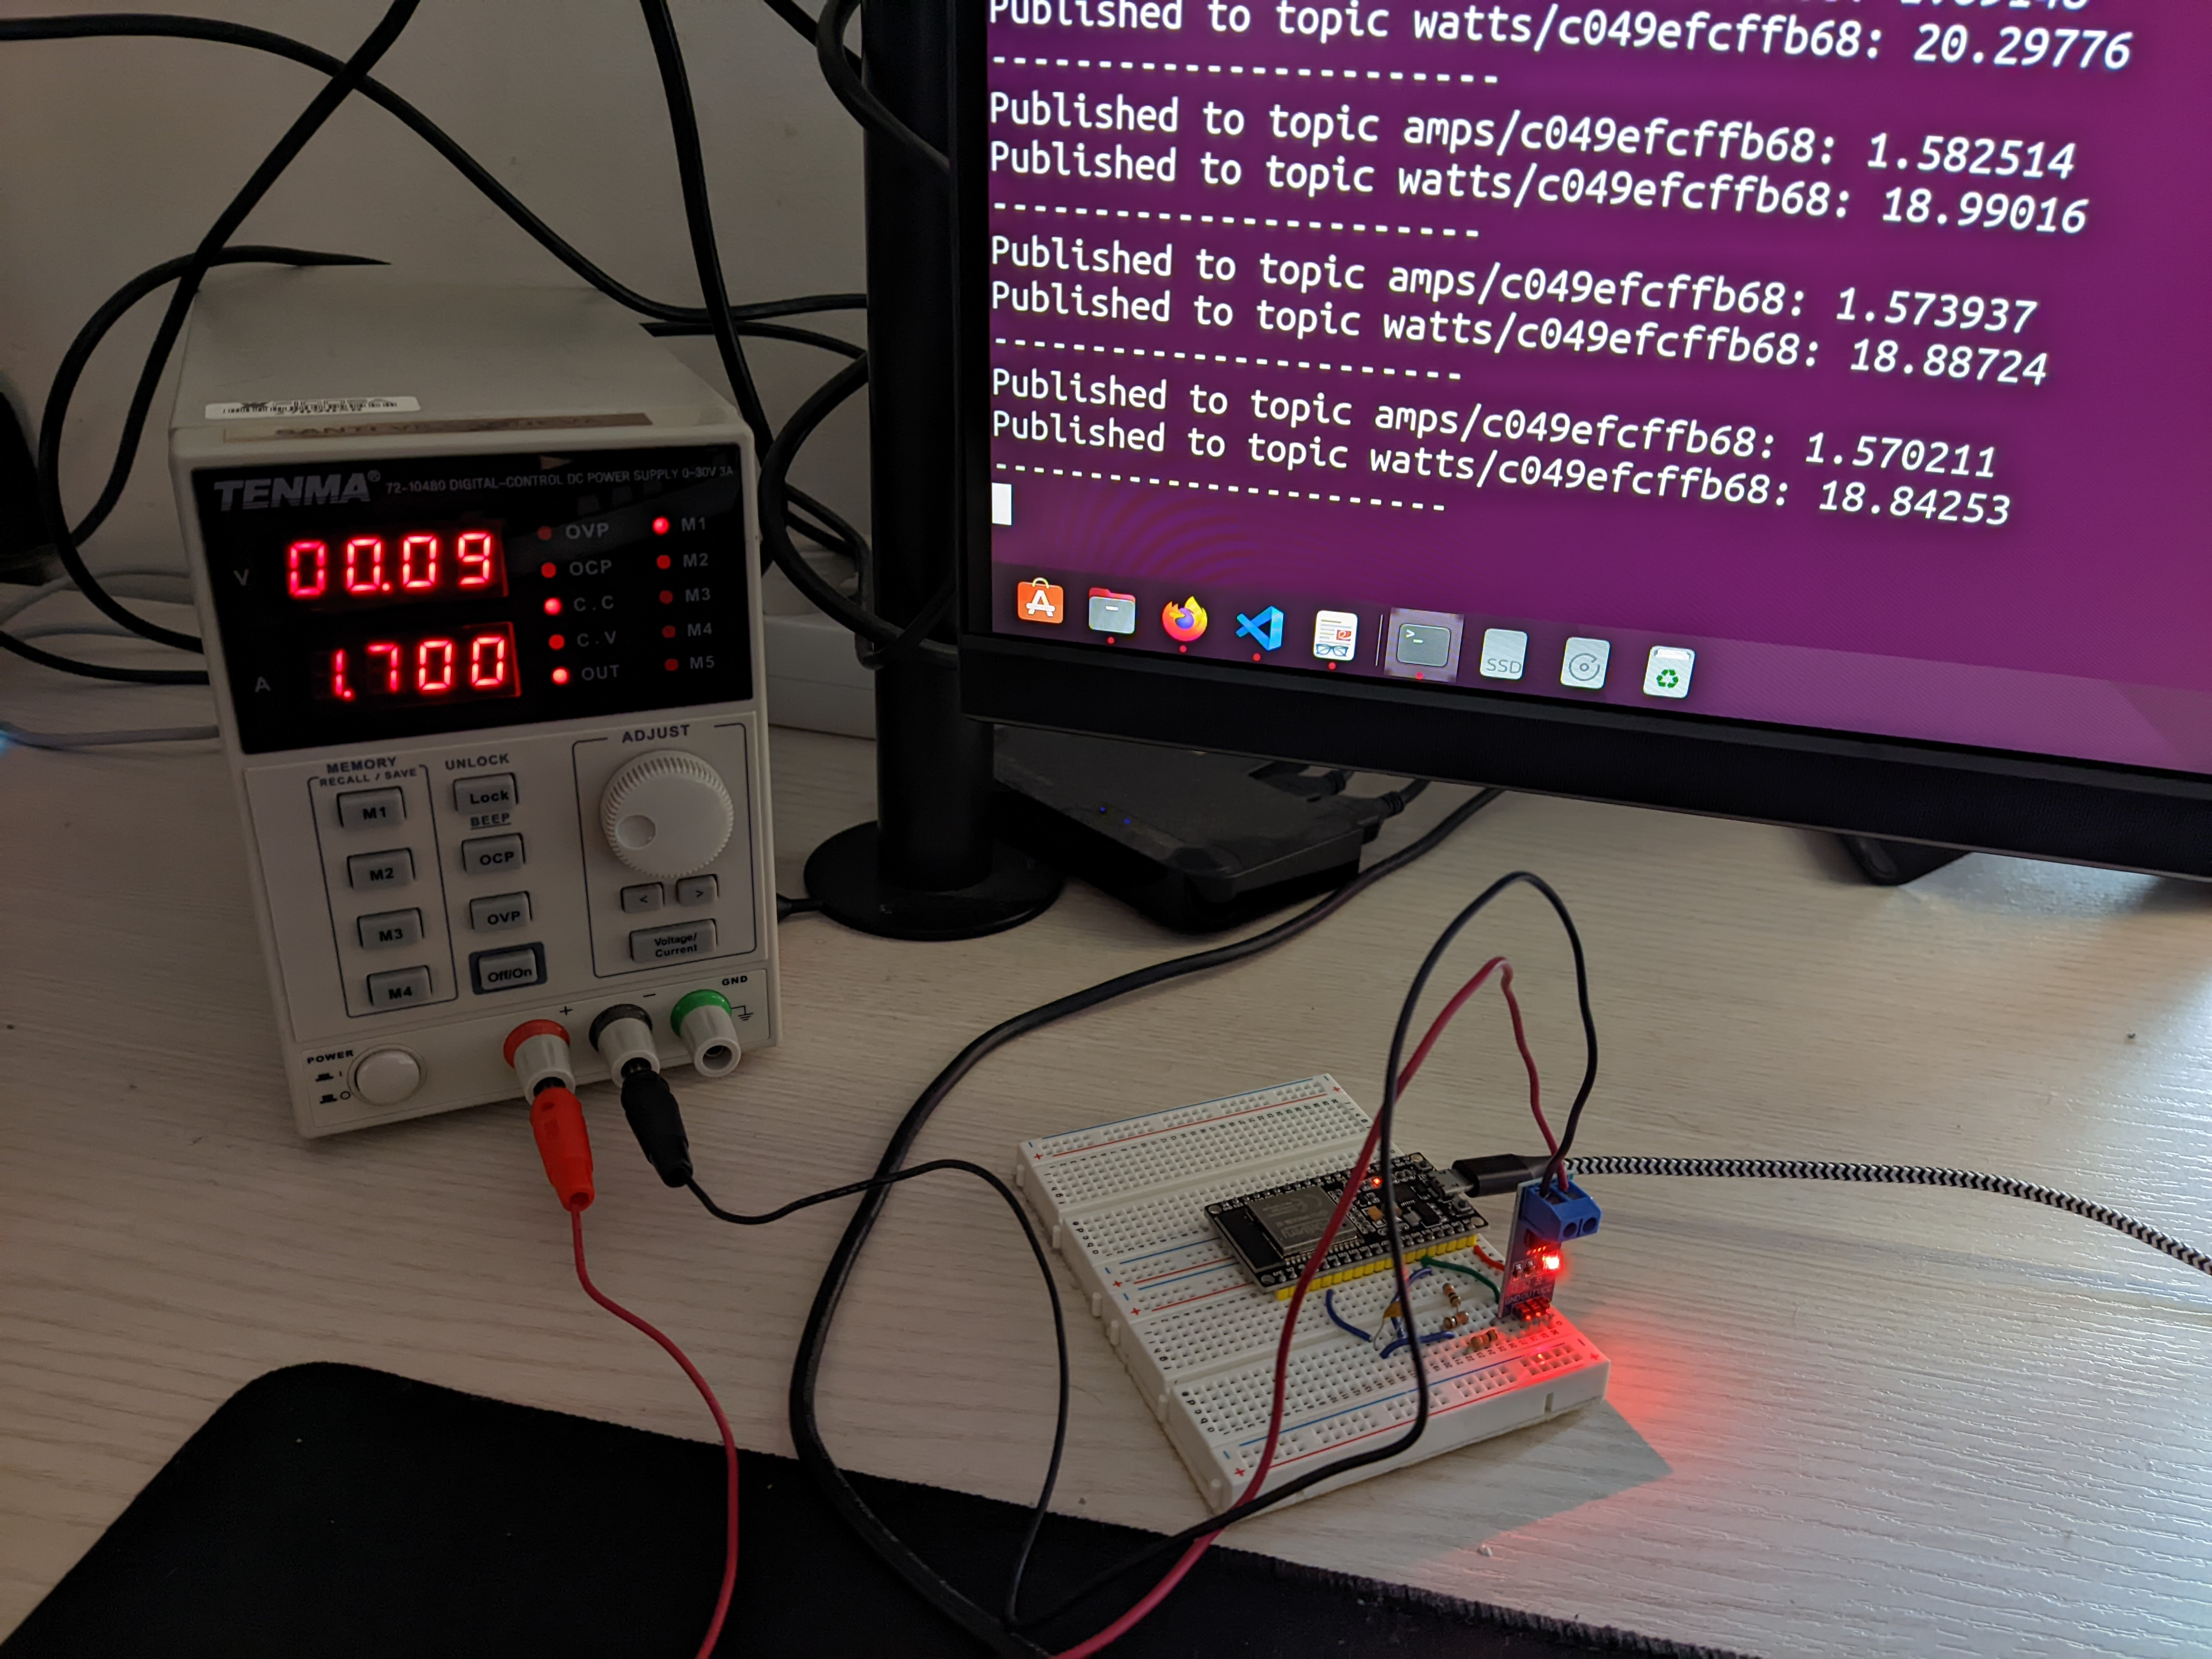
\includegraphics[width=0.5\textwidth]{imagenes/DC_1_7Amp.jpg}
	\caption{Salida del ACS712 con corriente continua de 1.7A}
\end{figure}
Generando 1.7A de corriente continua, medimos 1.58A con el sensor ACS712. \\
\subsubsection{3A}
\begin{figure}[h!]
	\centering
	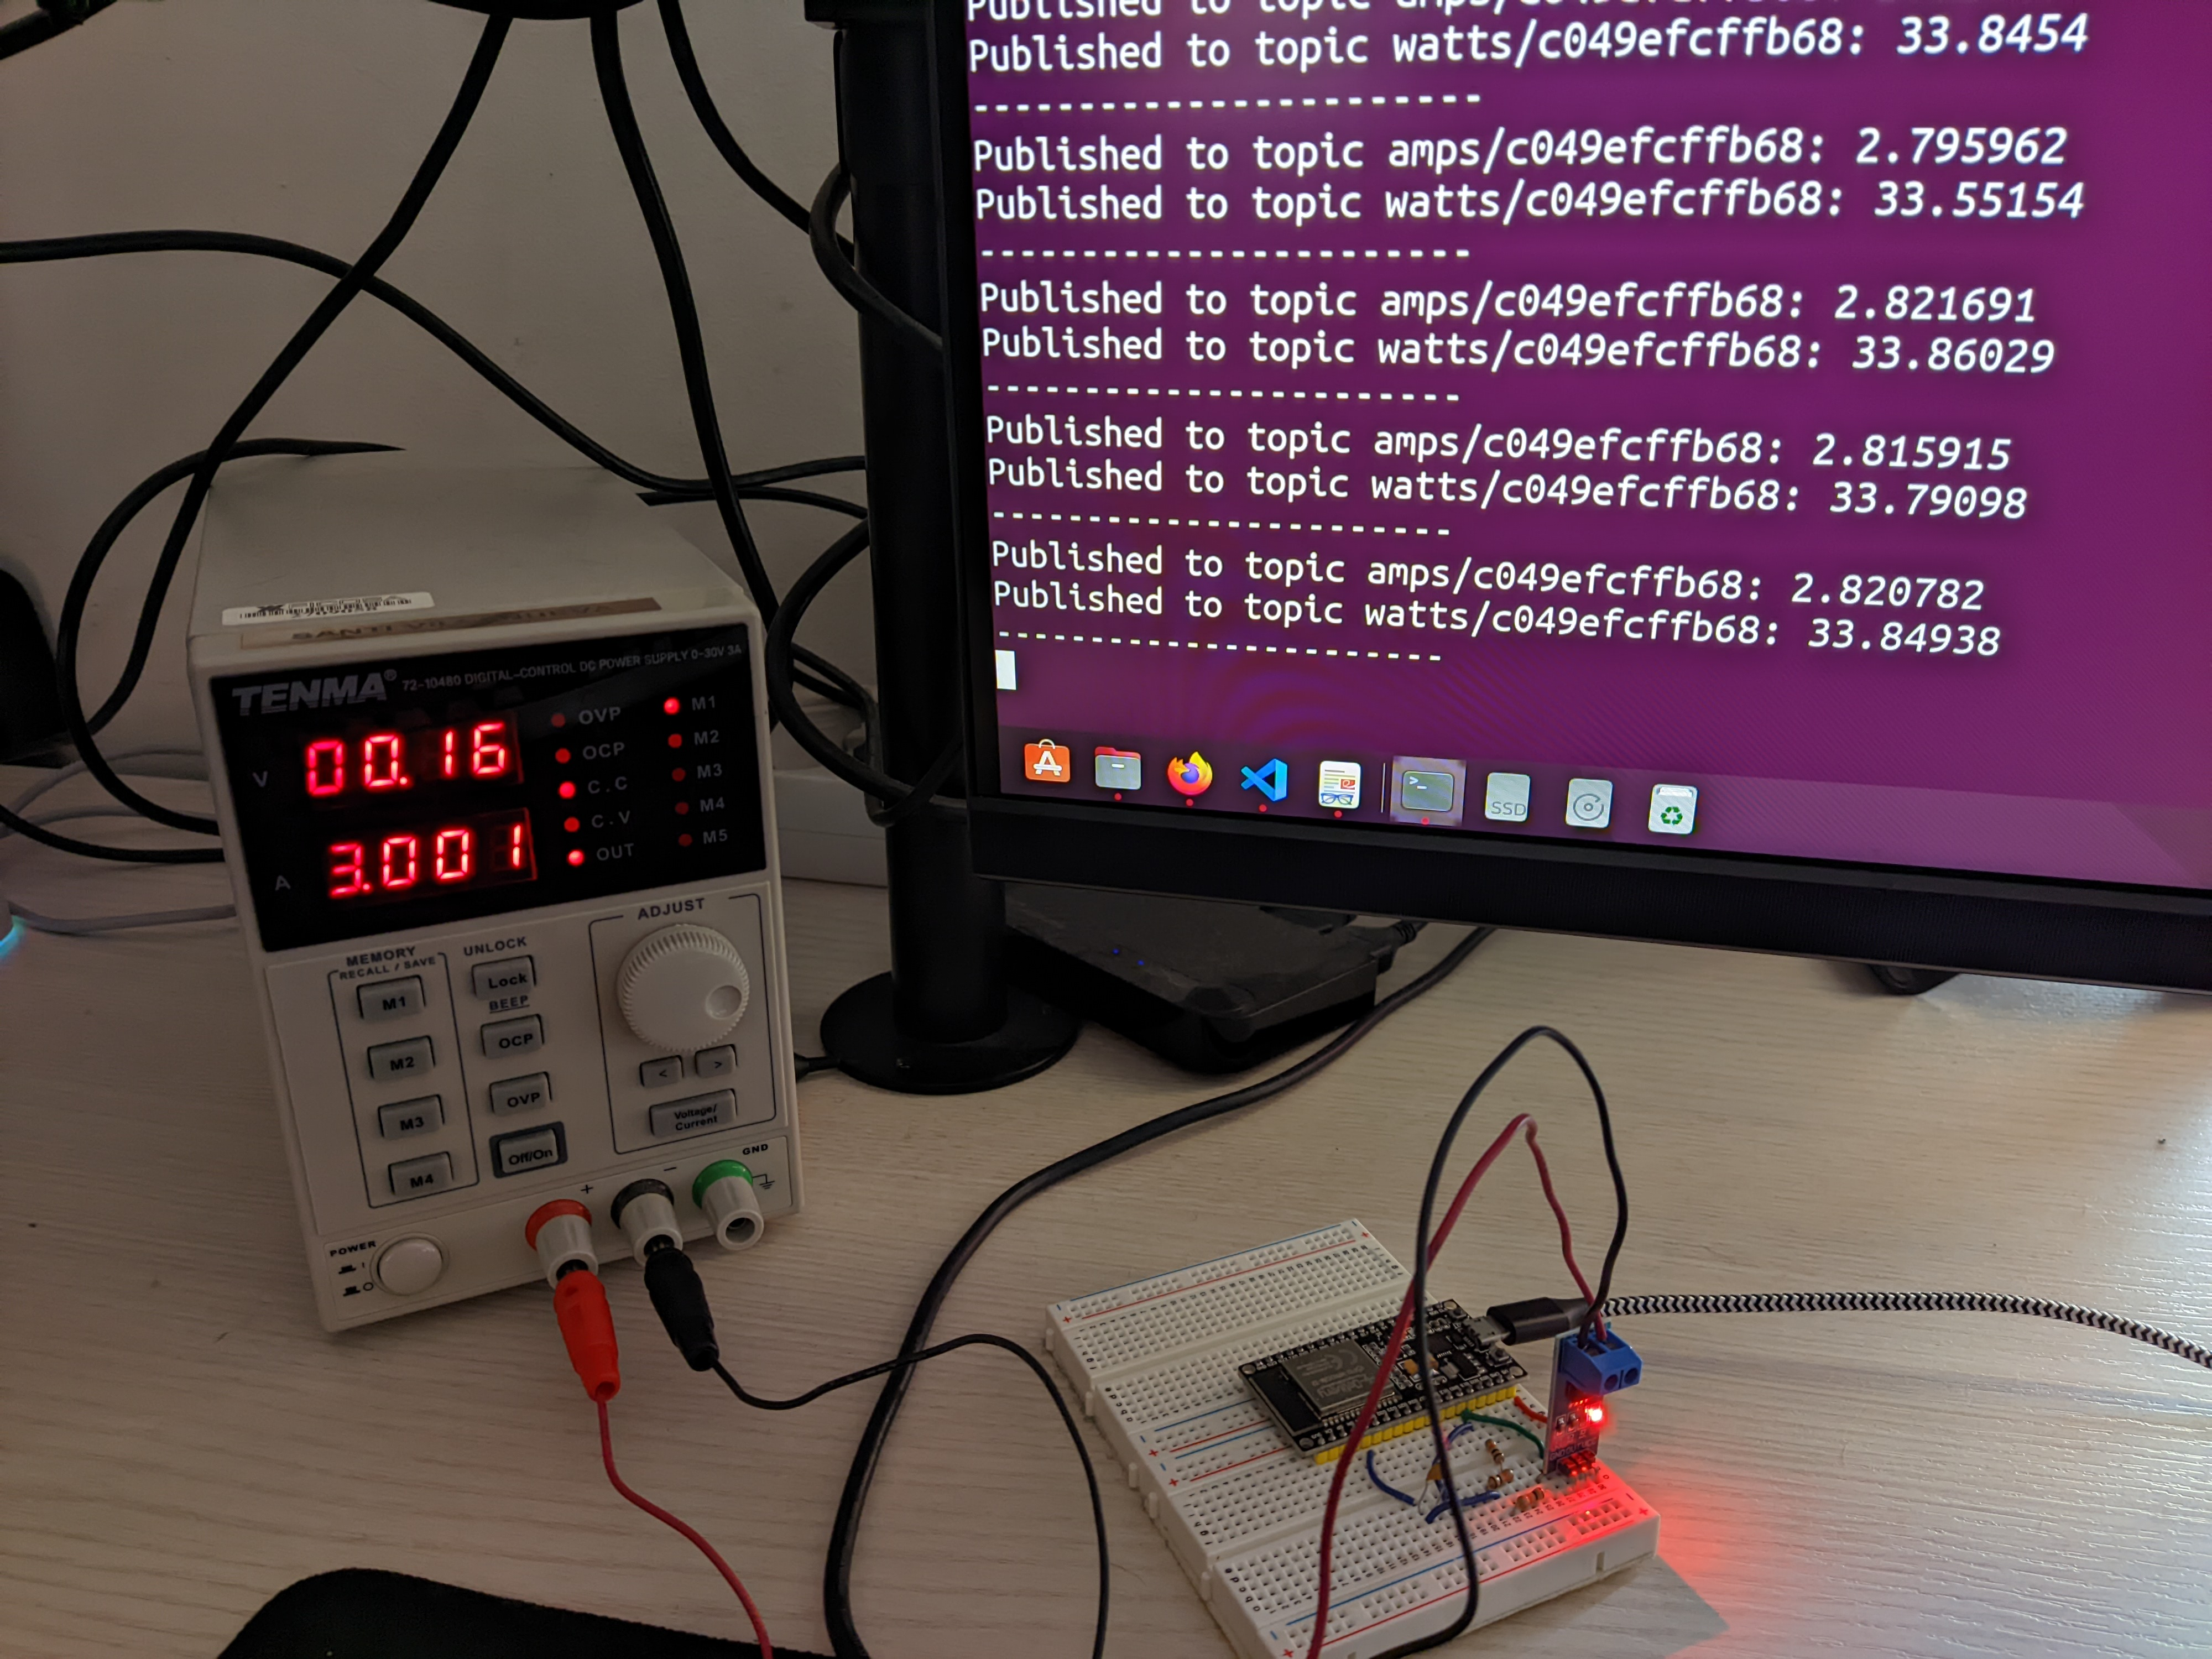
\includegraphics[width=0.5\textwidth]{imagenes/DC_3Amps.jpg}
	\caption{Salida del ACS712 con corriente continua de 3A}
\end{figure}
Generando 3A de corriente continua, medimos 2.82A con el sensor ACS712. \\

\subsection{Corriente alterna}
Como no dispongo de un generador de corriente alterna, he utilizado diferentes aparatos electricos para poder medir el consumo y el resultado del ACS712 se ha comparado con un amperimetro. El ACS712 esta conectado midiendo la corriente que pasa por el cable de una regleta de enchufes.\\
\subsubsection{No load}
Para la prueba de no tener ningun dispositivo conectado, simplemente se ha medido sin tener ningun enchufe conectado a la regleta.\\
\begin{figure}[h!]
	\centering
	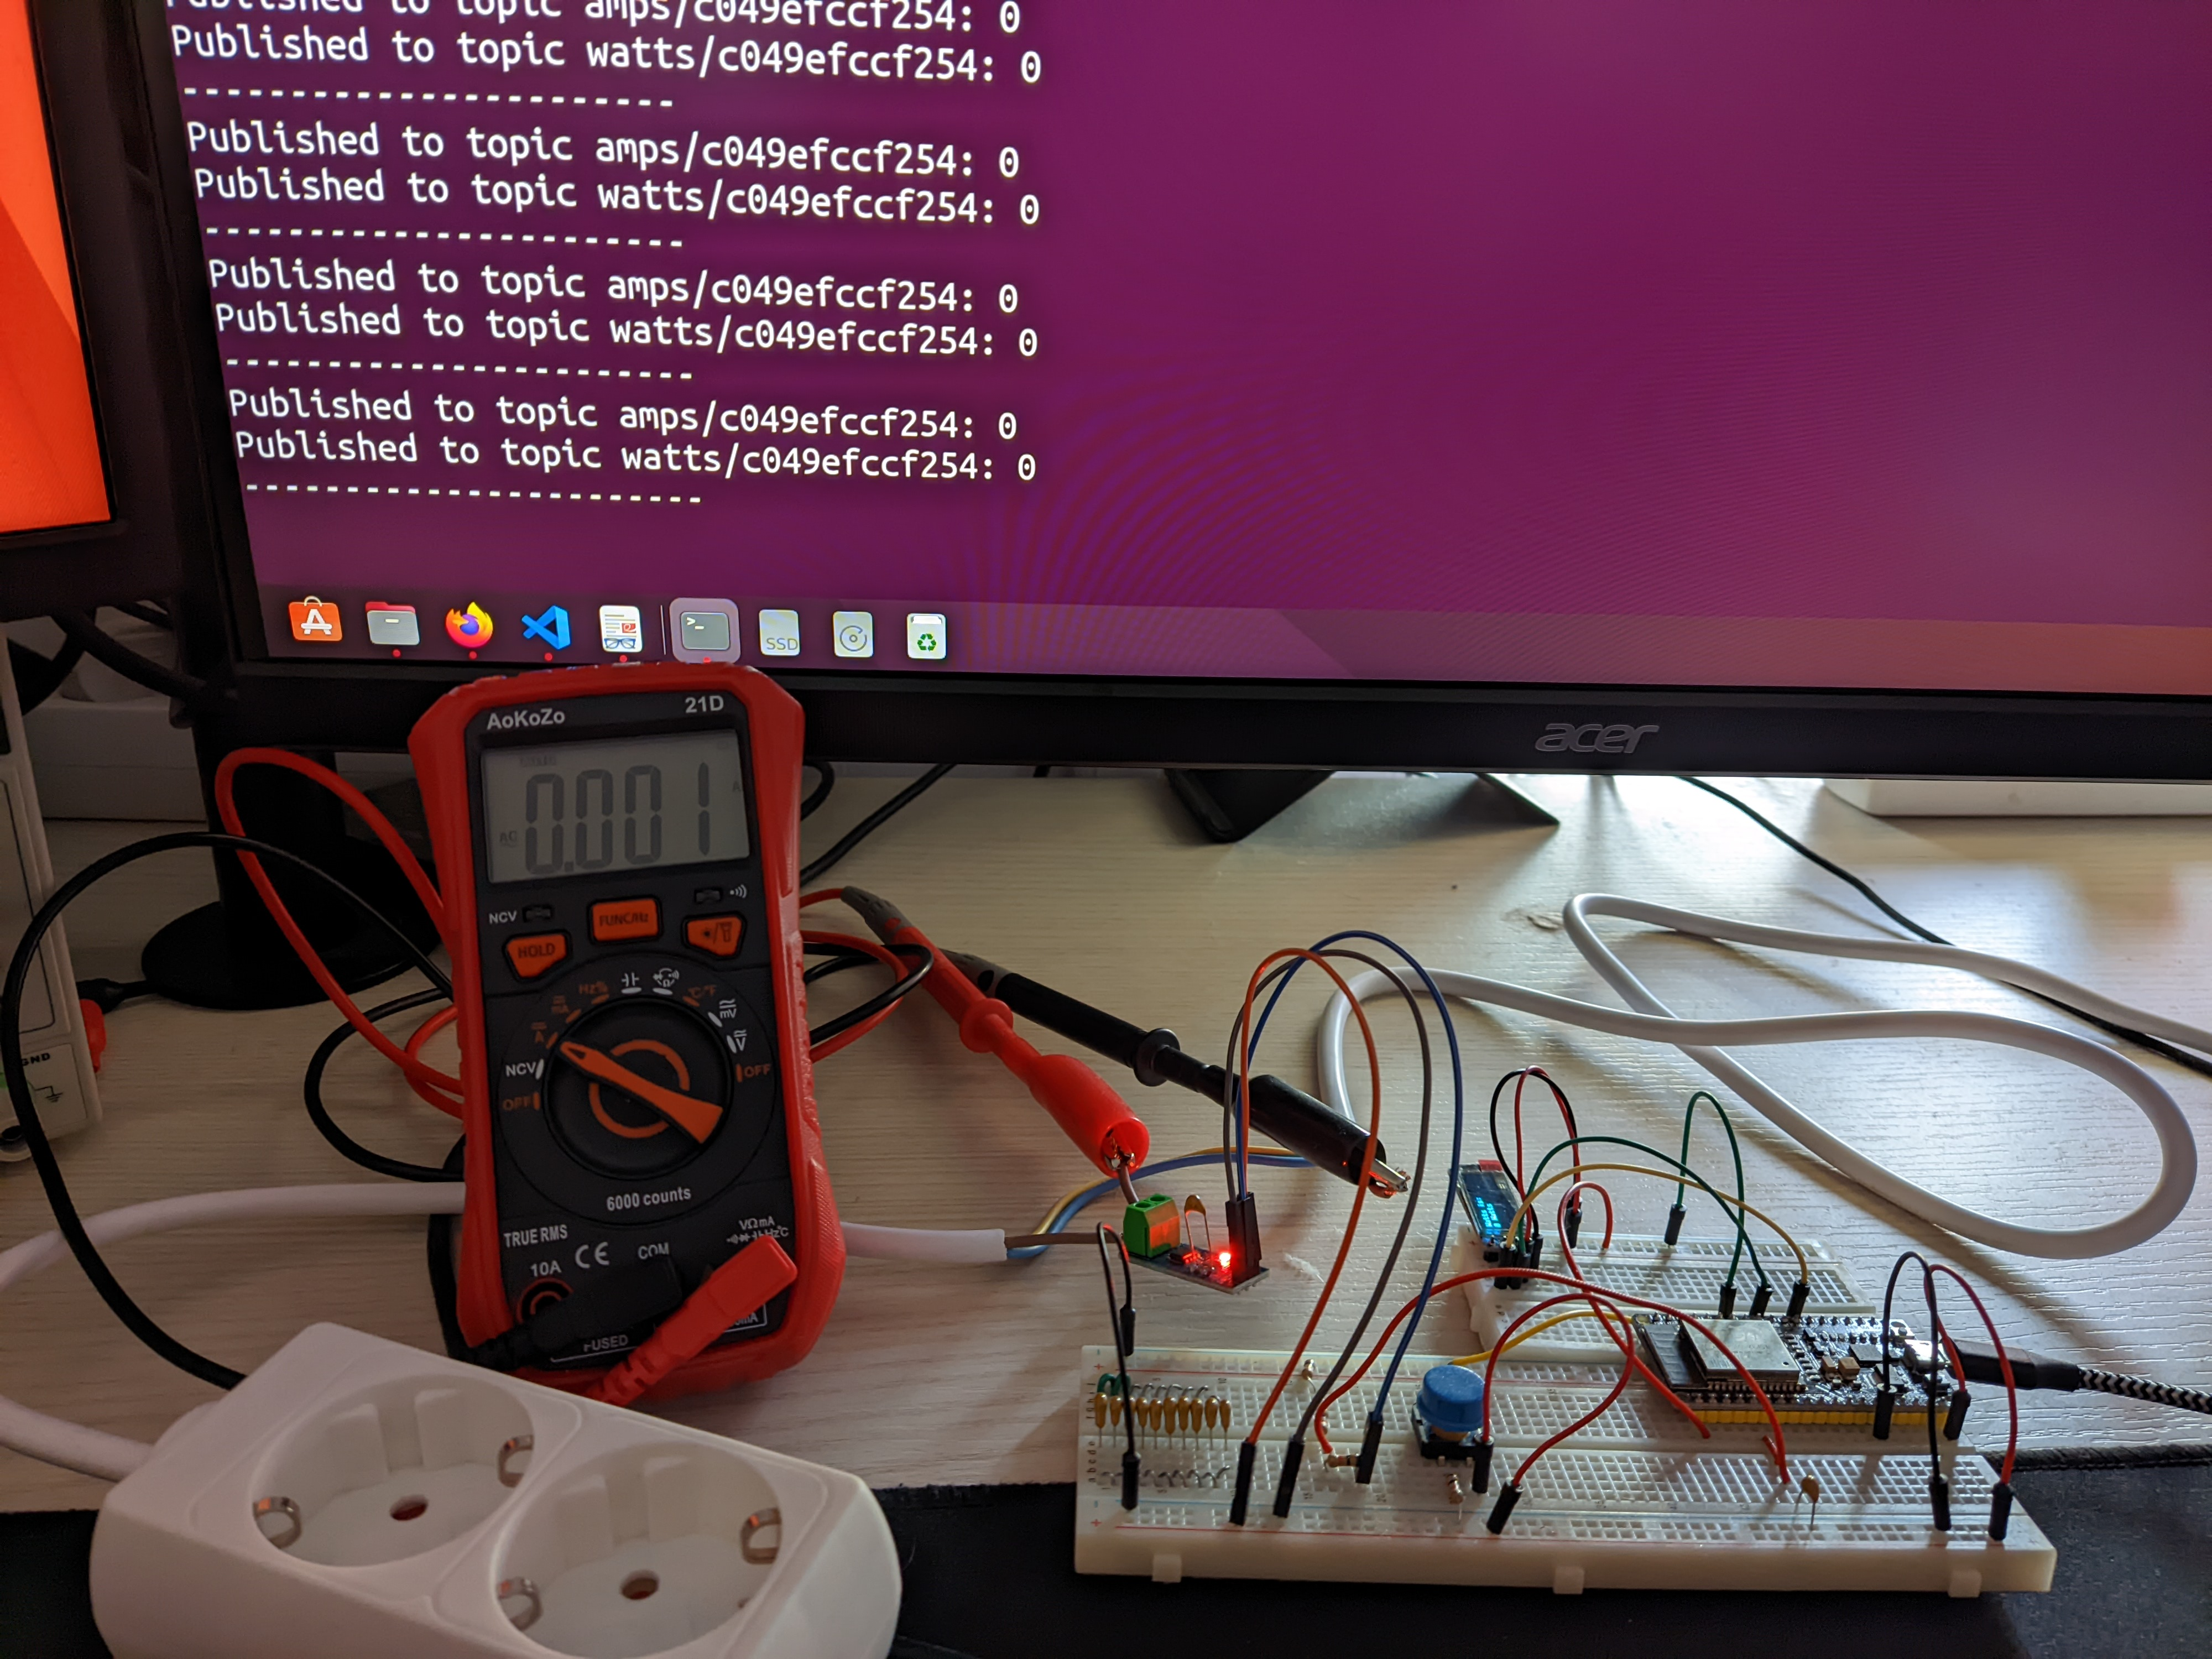
\includegraphics[width=0.5\textwidth]{imagenes/AC_noload.jpg}
	\caption{Nada conectado al enchufe}
\end{figure}
Como podemos observar, ACS712 nos da un valor de 0A al igual que el amperimetro.

\subsubsection{Secador aire frío}
La primera prueba con baja corriente se ha puesto un secador de pelo con la función de solo aire frio. Como solo esta funcionando el motor del secador, podemos observar como hay mas diferencia entre lo que mide el ACS712 y el amperimetro. \\
\begin{figure}[h!]
	\centering
	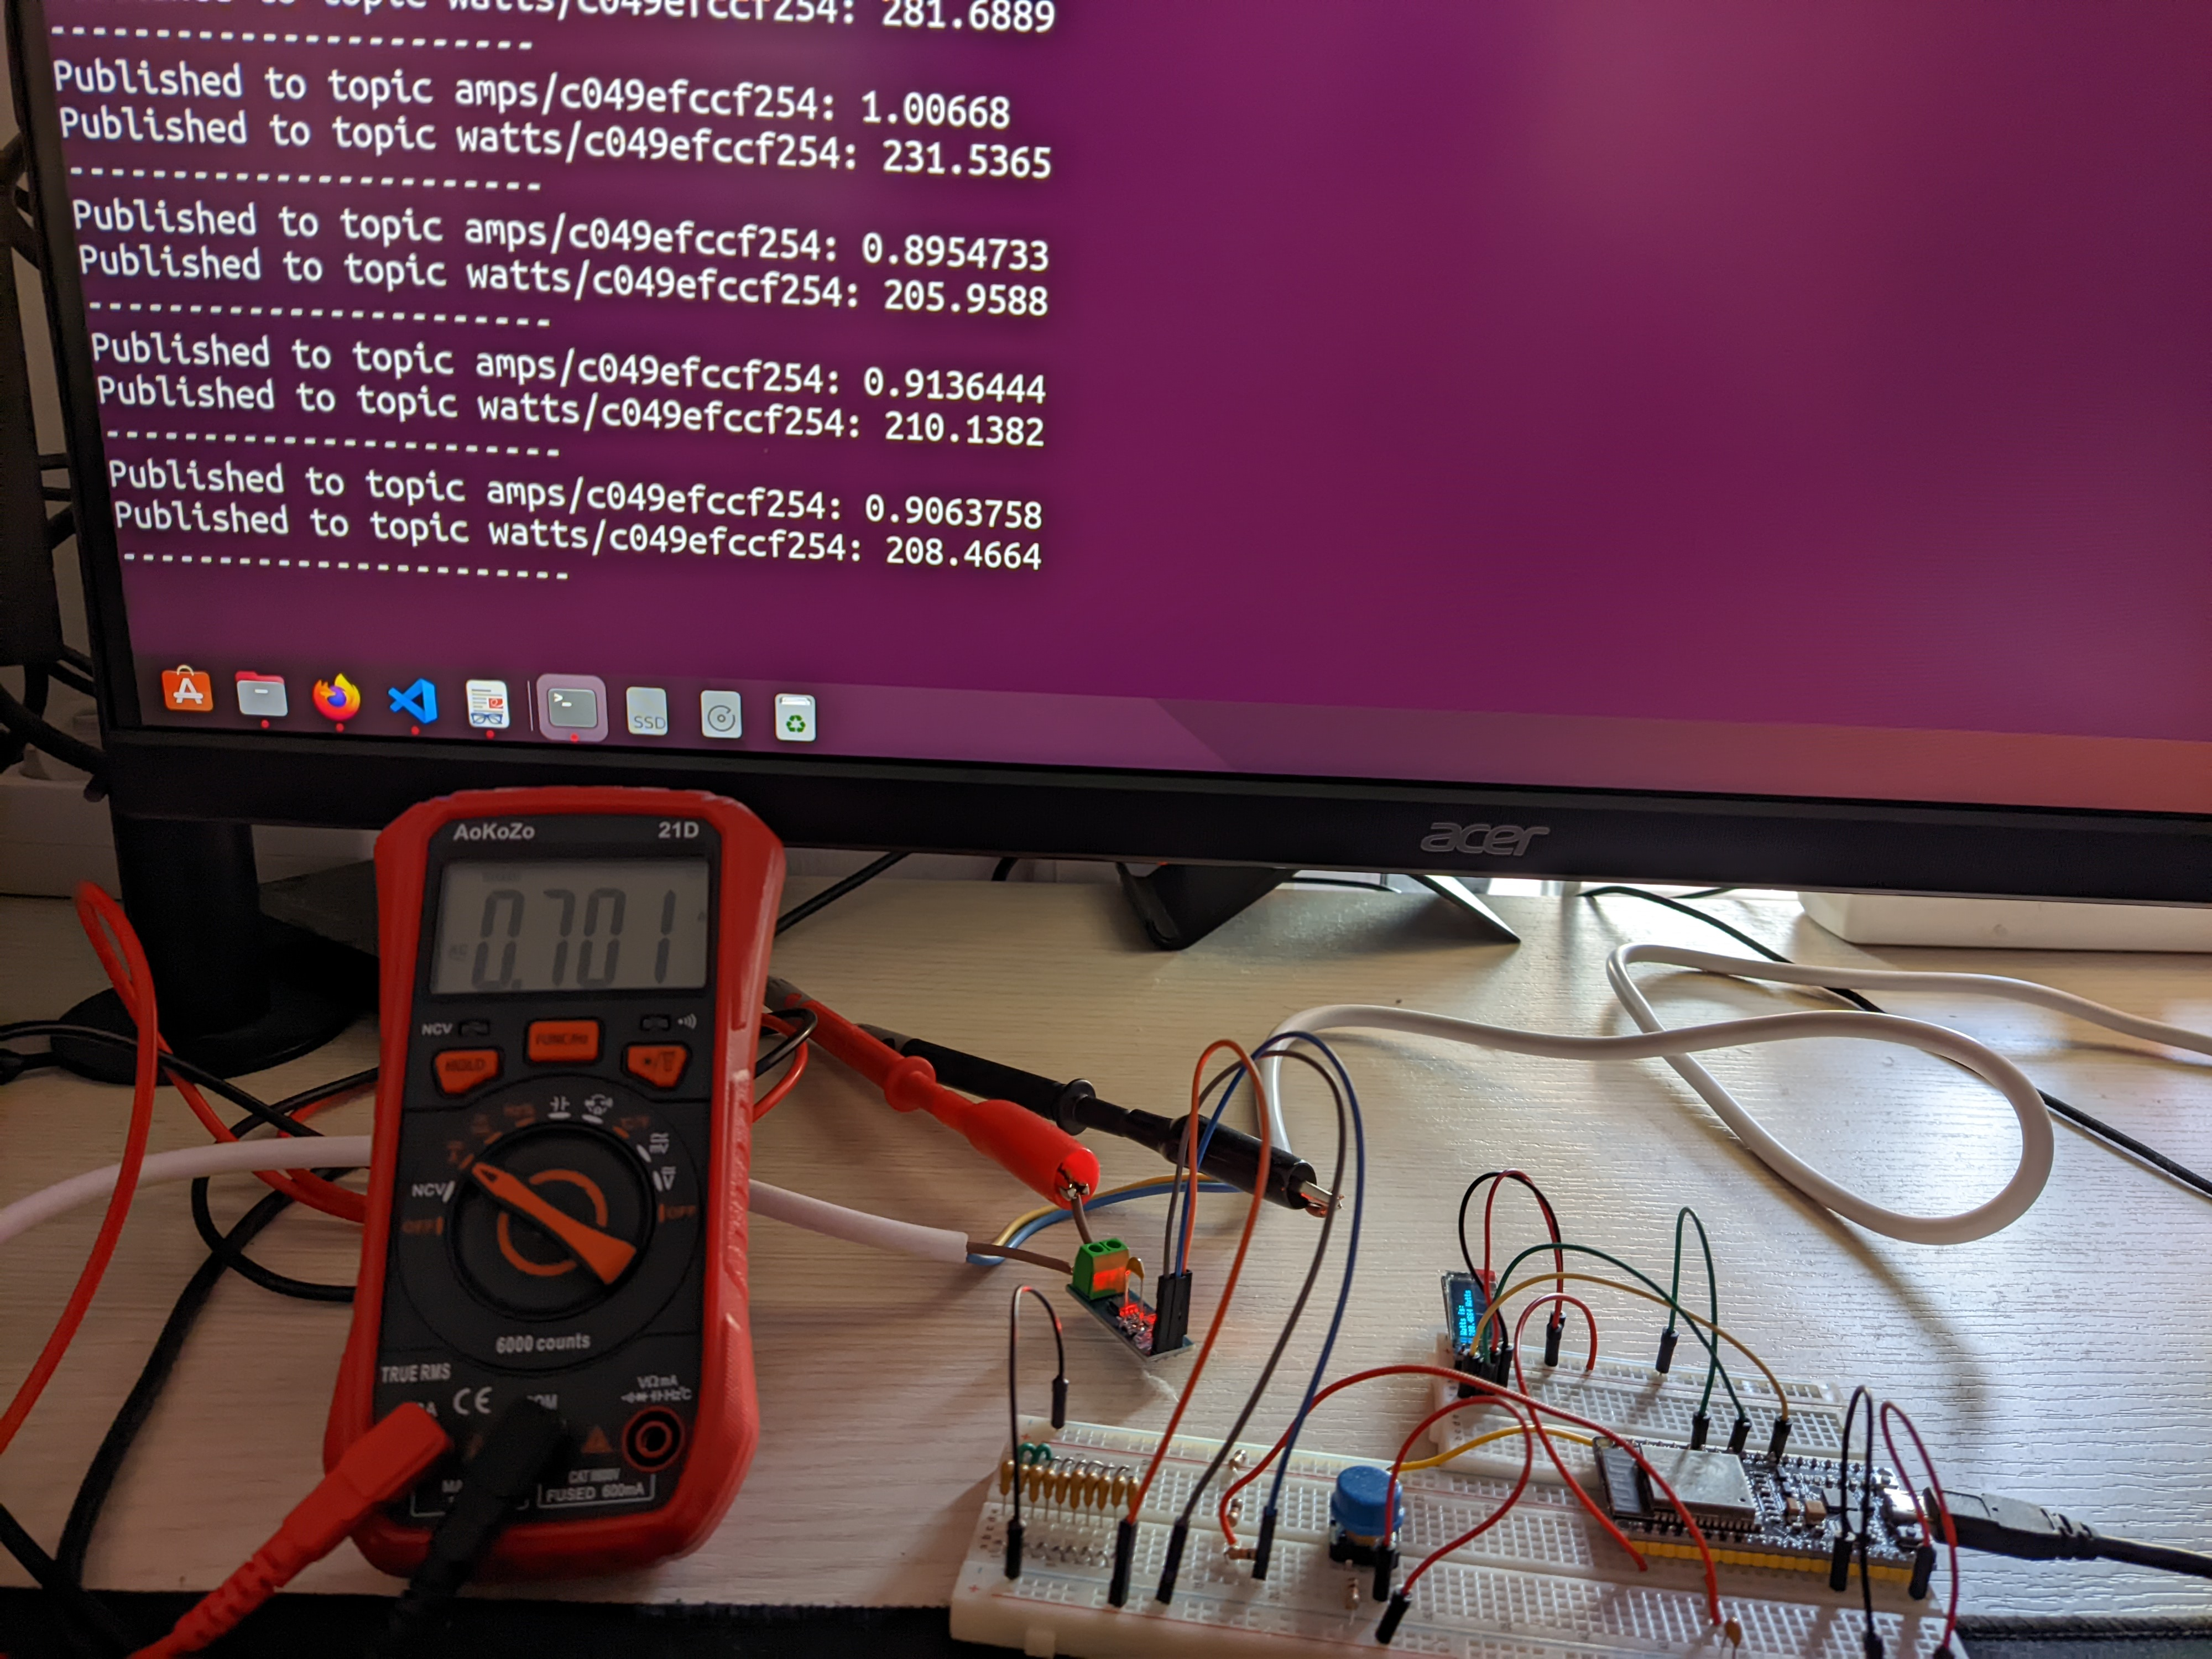
\includegraphics[width=0.5\textwidth]{imagenes/AC_O_7Amps.jpg}
	\caption{Secador de pelo solo con la función de aire frio}
\end{figure}
El amperimetro mide 0.701A y el ACS712 0.961A. \\

\subsubsection{Secador aire caliente al minimo}
La siguiente prueba la hacemos con el secador de pelo con la función de aire caliente pero a nivel bajo de calor.\\
\begin{figure}[h!]
	\centering
	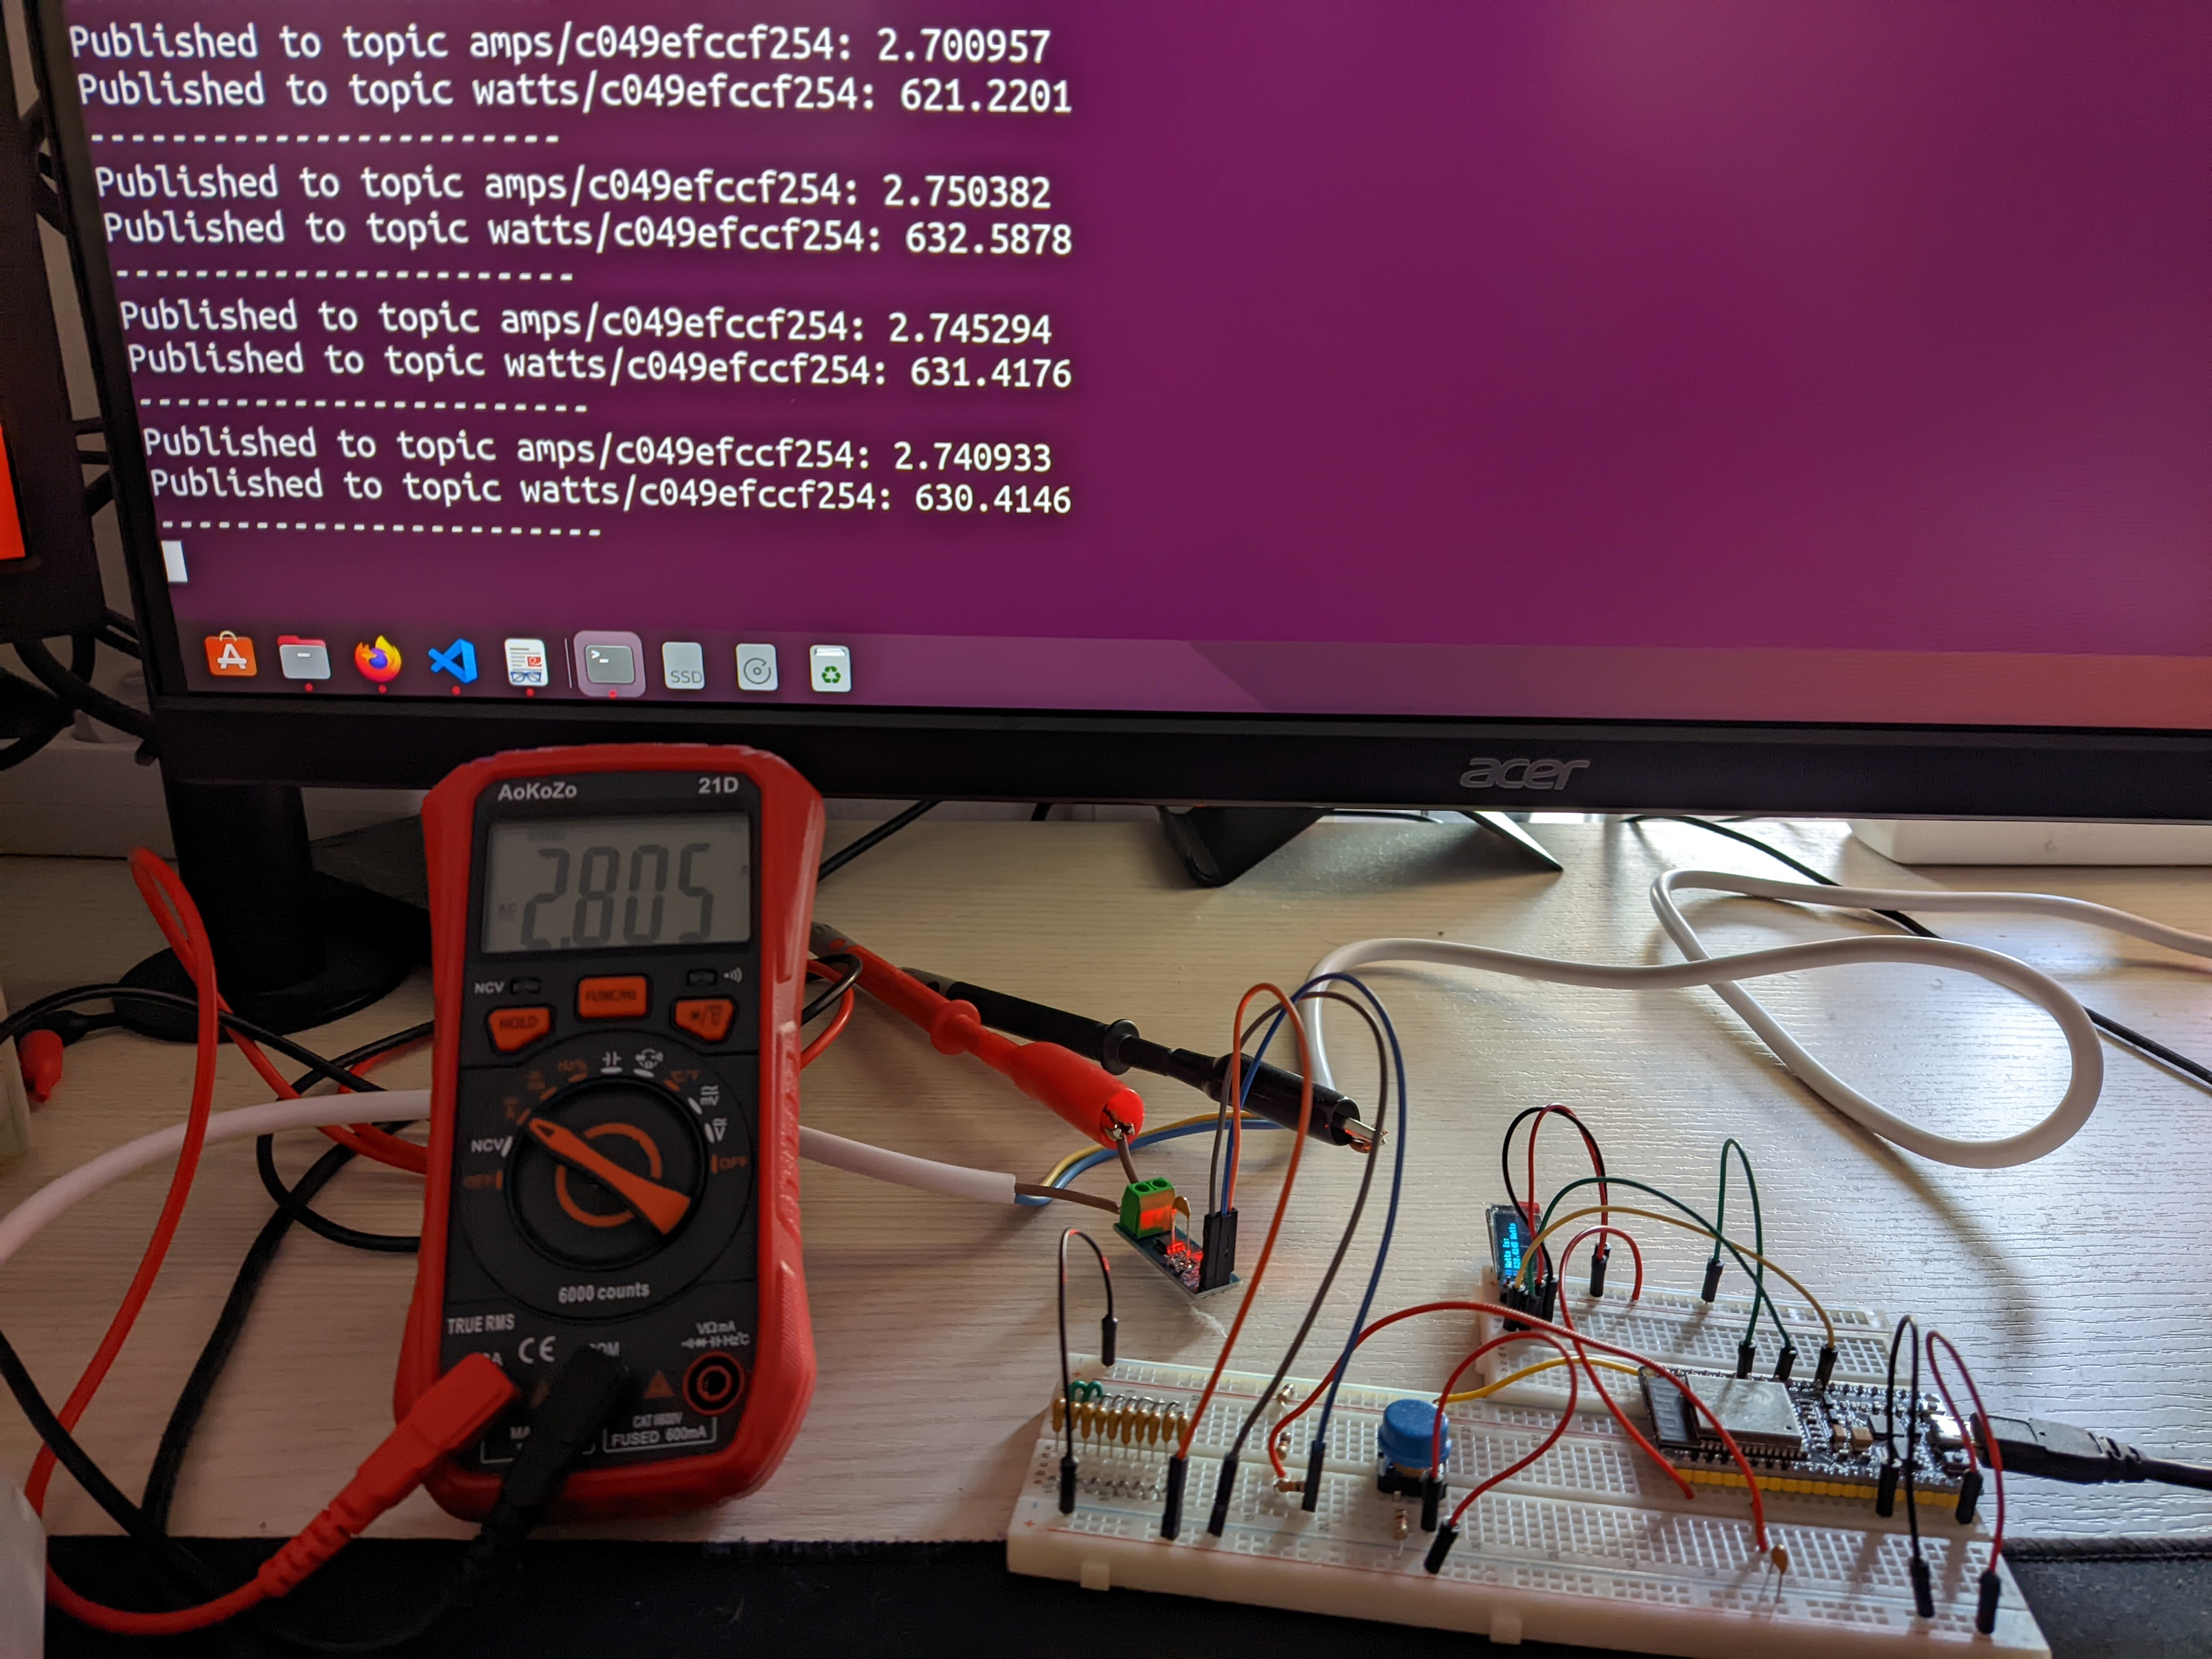
\includegraphics[width=0.5\textwidth]{imagenes/AC_2_8Amps.jpg}
	\caption{Secador de pelo solo con la función de aire caliente a nivel bajo de calor.}
\end{figure}
Al estar usando el secador las resistencias para generar aire caliente, podemos observar como aqui si que medimos con el ACS712 casi igual que con el amperimetro.
El amperimetro mide 2.8A y el ACS712 2.75A. \\
\subsubsection{Secador aire caliente al máximo}
La última prueba la hacemos con el secador de pelo con la función de aire caliente al máximo nivel de calor.\\
\begin{figure}[h!]
	\centering
	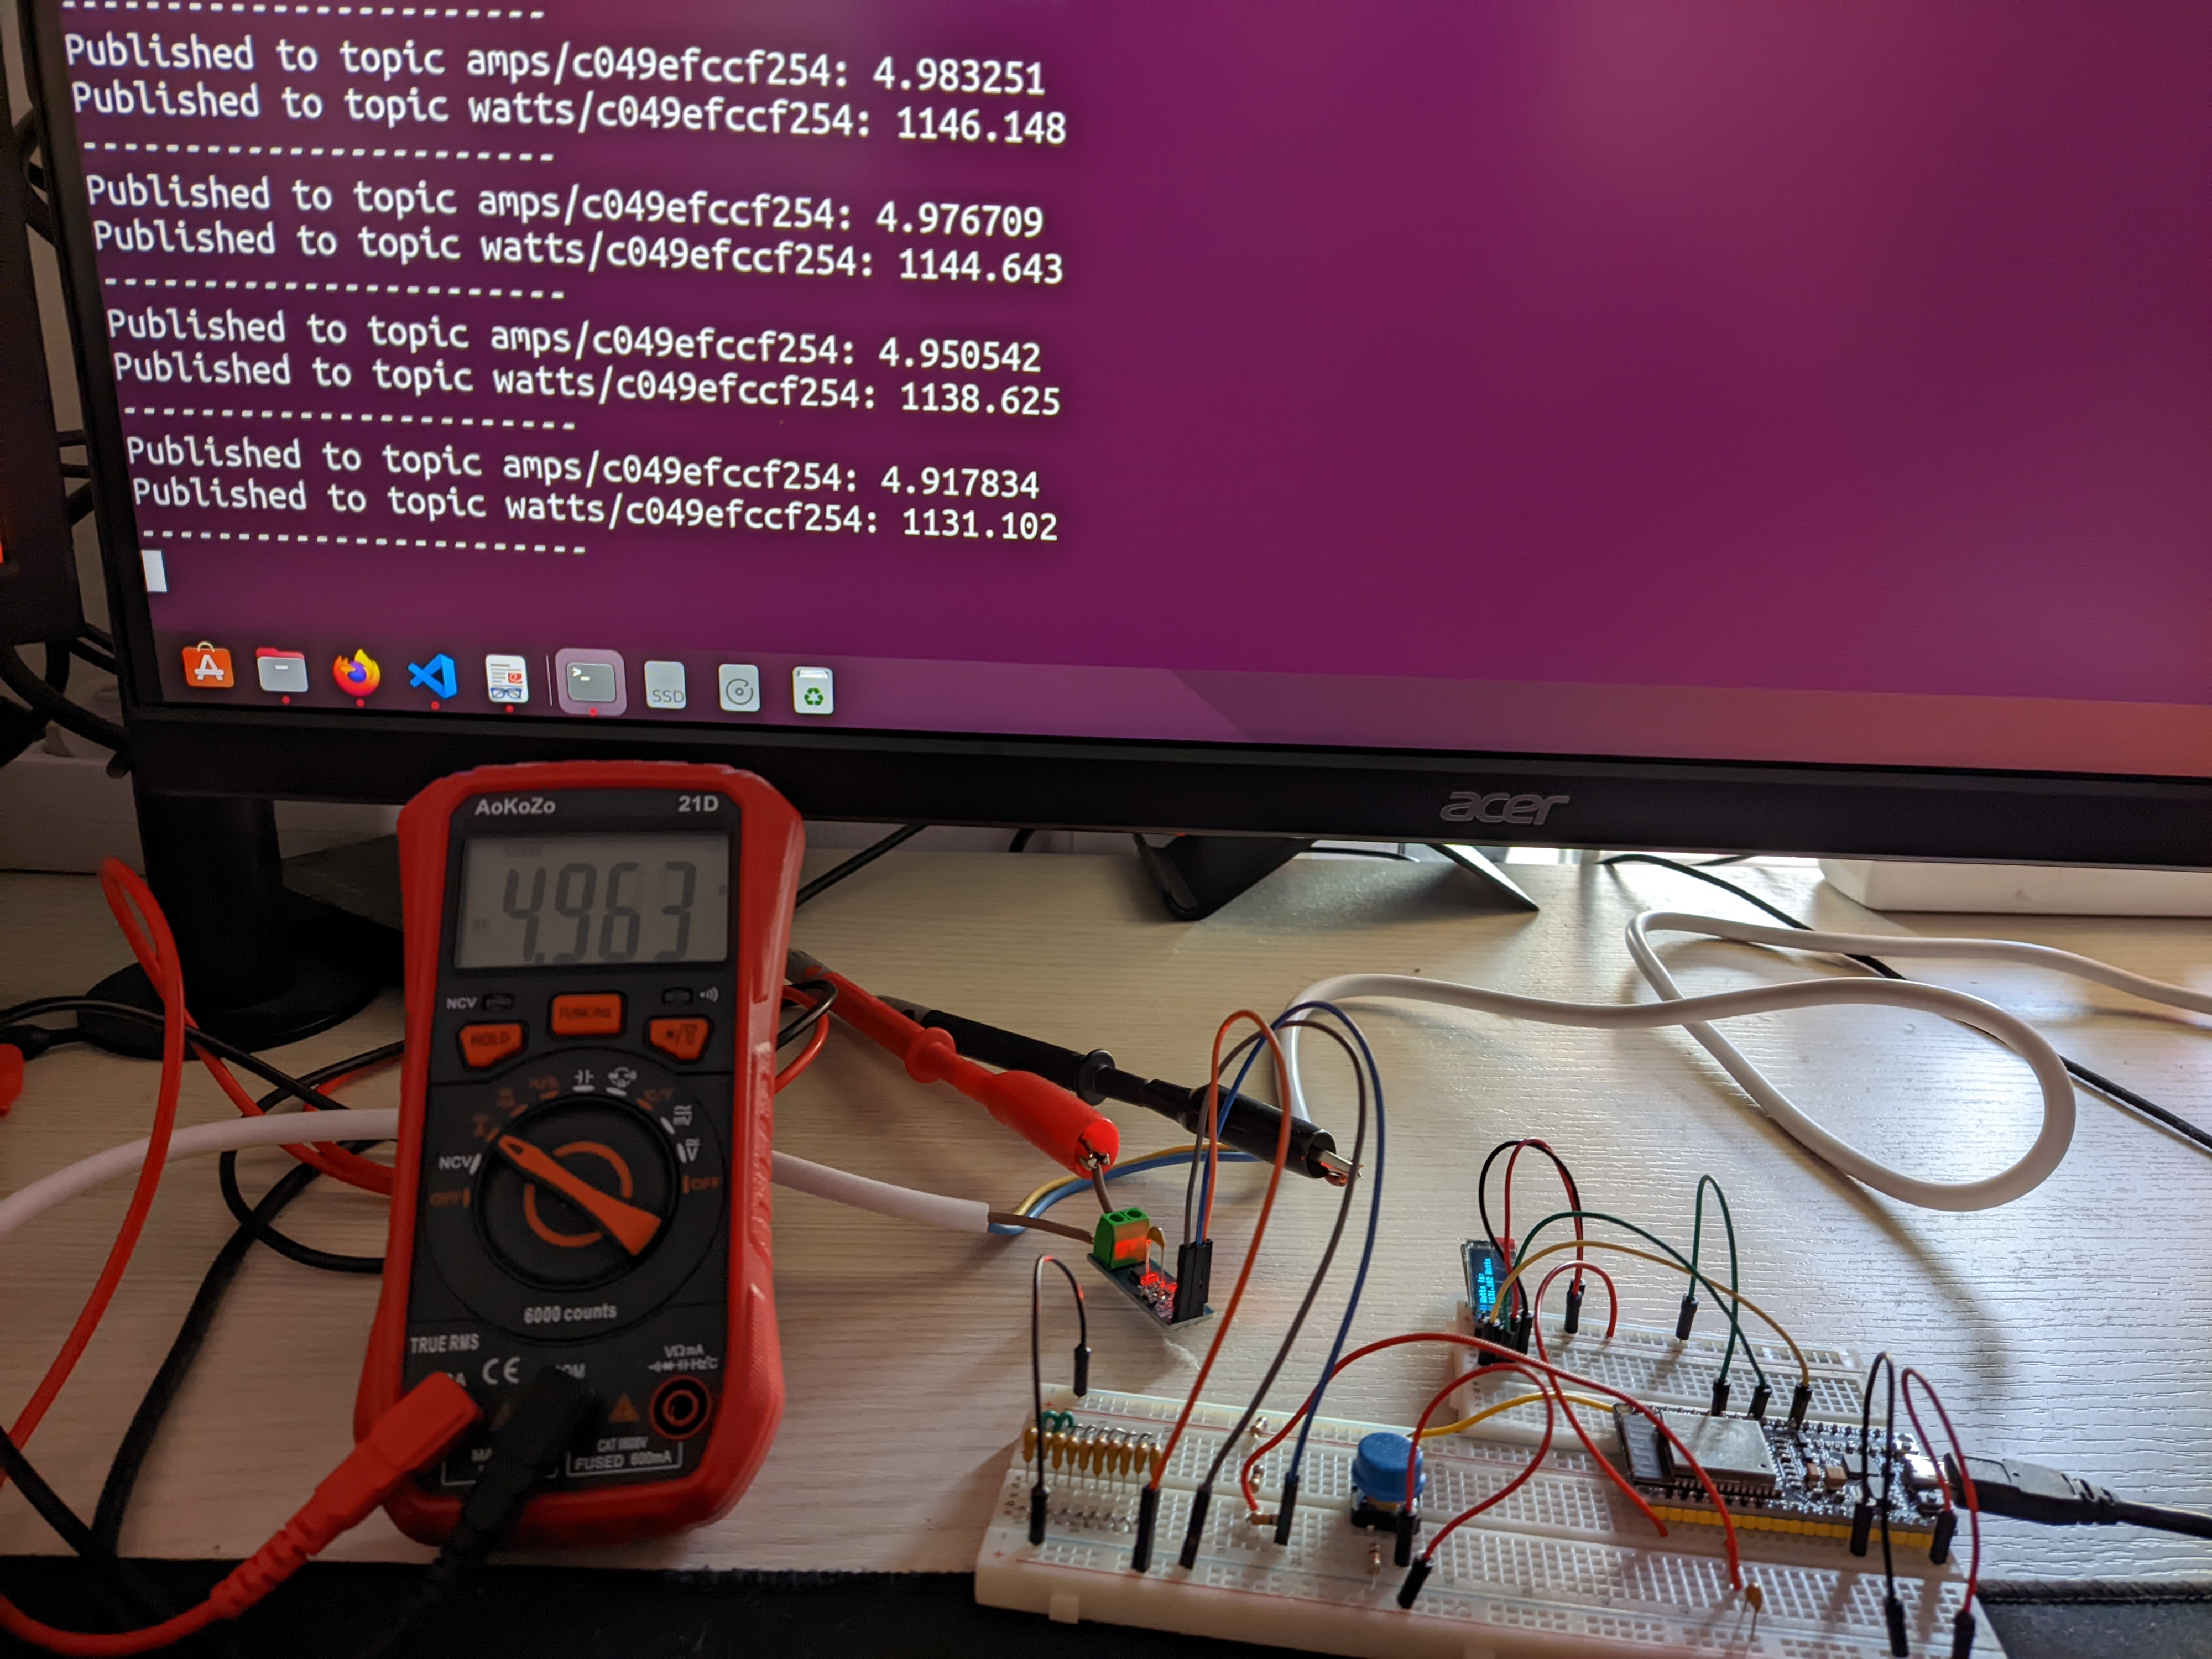
\includegraphics[width=0.5\textwidth]{imagenes/AC_4_9Amps.jpg}
	\caption{Secador de pelo solo con la función de aire caliente a nivel máximo de calor.}
\end{figure}
El ACS712 podemos observar como mide 4.95A y el amperimetro 4.963A.\\

\newpage
\end{titlepage}

%
\begin{titlepage}
\chapter{Implementación de la aplicación web}
\section{Descripción general}
El objetivo de la aplicación web es que sirva de interfaz para mostrar los datos recopilados de todos los sensores que se encuentren configurados en la red. 
\section{Implementación backend}
El backend de la aplicación web se ha implementado en Python utilizando el framework Flask, SocketIO y Paho para MQTT. Flask permite crear aplicaciones web de forma rápida y sencilla. SocketIO permite que la aplicación web sea capaz de recibir mensajes en tiempo real y comunicarse de forma facil con el cliente. Paho es una librería para MQTT que permite conectarse a un broker MQTT y publicar y suscribirse a topics.
\subsection{Aplicación en python3}
\subsubsection{Configuración de Flask}
Con la siguiente configuración, creamos una aplicación FLask pudiendo indicarle a la vez toda la configuración MQTT a usar.
\begin{lstlisting}[language=python]
	app = Flask(__name__)
	app.config['SECRET'] = 'my secret key'
	app.config['TEMPLATES_AUTO_RELOAD'] = True
	app.config['MQTT_BROKER_URL'] = '192.168.1.200'
	app.config['MQTT_BROKER_PORT'] = 1883
	app.config['MQTT_CLIENT_ID'] = 'APP_SERVER'
	app.config['MQTT_CLEAN_SESSION'] = True
	app.config['MQTT_USERNAME'] = 'pi'
	app.config['MQTT_PASSWORD'] = 'nairda'
	app.config['MQTT_KEEPALIVE'] = 5
	app.config['MQTT_TLS_ENABLED'] = False
	app.config['MQTT_LAST_WILL_TOPIC'] = 'home/lastwill'
	app.config['MQTT_LAST_WILL_MESSAGE'] = 'bye'
	app.config['MQTT_LAST_WILL_QOS'] = 2
\end{lstlisting}

\subsubsection{Background tasks}
Esta clase se encarga de ejecutar las tareas en segundo plano. Una tarea ira actualizando periodicamente el coste de la electricidad, y la otra tarea se ejecutara cuando sea necesario enviar la configuración a un sensor por MQTT.\\
\begin{lstlisting}[language=python]
class backgroundTask():
    def __init__(self):
        self.sendConfigToSensor = False

    def stop_sendConfigToSensor(self):
        logging.debug('stop_sendConfigToSensor called')
        self.sendConfigToSensor = False

    def start_sendConfigToSensor(self, json_data):
        self.sendConfigToSensor = True
        data = json.loads(json_data)
        logging.info("Starting background thread to send config to sensor")
        while self.sendConfigToSensor:
            logging.info("Running loop to send config to sensor")
            logging.info('Sending config to sensor %s', \
			data['sensor_type'] + ',' + data['voltage'])
            mqtt.publish('sensor_config/' + data['sensor_id'], \
			data['sensor_type'] + ',' + data['voltage'])
            socketio.sleep(1)
    
    def update_cost_electricity(self):
        
        while True:
            costElectricity.load_current_data()
            logging.debug("Reloading cost electricity data :", 
			costElectricity.current_data)
            #notify socket new data
            socketio.emit('cost_electricity', costElectricity.current_data)
            socketio.sleep(60)
\end{lstlisting}

\subsubsection{Clase para gestionar los sensores}
Esta clase se encarga de gestionar los sensores, almacenando los datos de los sensores en un JSON. Tenemos una para añadir un sensor al JSON, otra función para leer los sensores del JSON y otra para eliminar un sensor del JSON.\\

\begin{lstlisting}[language=python]
class handleSensors():
    def __init__(self):
        self.JSON_FILE = 'sensors.json'
        self.sensors_data = None
    
    def read_saved_sensors(self):
        if os.path.isfile(self.JSON_FILE):
            with open(self.JSON_FILE, "r") as f:
                self.sensors_data = json.load(f)
                print(self.sensors_data)
        else:
            with open(self.JSON_FILE, "w", encoding='utf-8') as f:
                json.dump({}, f, ensure_ascii=False, indent=4)
            logging.debug("No sensors found")

    def add_sensor(self, sensor):
        with open(self.JSON_FILE, "r") as f:
            json_sensors = json.load(f)
            sensorFound = False
            for sensor_id, sensor_data in json_sensors.items():
                print("sensor_id: ", sensor_id, "sensor_type: ", 
				sensor_data["sensor_type"])

            if not sensorFound:
                logging.debug("New sensor added: %s", sensor["sensor_id"])
                json_sensors[sensor["sensor_id"]] = sensor
                self.sensors_data = json_sensors
                with open(self.JSON_FILE, "w", encoding='utf-8') as f:
                    json.dump(json_sensors, f, ensure_ascii=False, indent=4)
                #after adding, subscribe to watts topic
                mqtt.subscribe('watts/' + sensor["sensor_id"])
    
    def remove_sensor(self, sensor_id):
        with open(self.JSON_FILE, "r") as f:
            json_sensors = json.load(f)
            json_sensors.pop(sensor_id)
            self.sensors_data = json_sensors
            with open(self.JSON_FILE, "w", encoding='utf-8') as f:
                json.dump(json_sensors, f, ensure_ascii=False, indent=4)
            #after removing, unsubscribe to watts topic
            mqtt.unsubscribe('watts/' + sensor_id)
\end{lstlisting}

\subsubsection{Funciones de la APP FLask}
Cada vez que un cliente pida una dirección de la web, estas son las funciones que se ejecutan, que tan solo llaman a renderizar plantillas html.\\
\begin{lstlisting}[language=python]
@app.route('/')
def index():
	return render_template('index.html')

@app.route('/add_sensor')
def add_sensor():
	return render_template('add_sensor.html')

@app.route('/sensors')
def sensors():
	print("sensors " + str(handleSensors.sensors_data))
	return render_template('sensors.html', 
	sensors=handleSensors.sensors_data)

@app.route('/sensors/<path:sensor_id>')
def sensor(sensor_id):
	return render_template('display_sensor_data.html', 
	data=handleSensors.sensors_data[sensor_id])
\end{lstlisting}

\subsubsection{Llamadas a socketio}
Estas son las llamadas a socketio que se ejecutan cuando se produce un evento. Para cada evento, se ejecutan diferentes acciones. Los eventos los pueden haber generado los clientes o la propia aplicación llamando a socketio.emit('EVENTO').\\
\begin{lstlisting}[language=python]
@socketio.on('publish')
def handle_publish(json_str):
	data = json.loads(json_str)
	mqtt.publish(data['topic'], data['message'], data['qos'])


@socketio.on('subscribe')
def handle_subscribe(json_str):
	data = json.loads(json_str)
	mqtt.subscribe(data['topic'], data['qos'])

@socketio.on('submit_sensor')
def handle_submit_sensor(json_str):
	data = json.loads(json_str)
	logging.info("New sensor added: %s", data['sensor_id'])
	mqtt.publish('ack/' + data['sensor_id'], "ack", 0)
	backgroundTask.start_sendConfigToSensor(json_str)
	handleSensors.add_sensor(data)

@socketio.on('stop_sending_config')
def handle_stop_sending_config():
	backgroundTask.stop_sendConfigToSensor()

@socketio.on('reset_sensor')
def handle_reset_sensor(str):
	logging.debug("Reset sensor: %s", str)
	mqtt.publish('restart/' + str, "restart", 0)

@socketio.on('calibrate_sensor')
def handle_calibrate_sensor(str):
	logging.debug("Recalibrating sensor: %s", str)
	mqtt.publish('calibrate/' + str, "reset", 0)

@socketio.on('delete_sensor')
def handle_delete_sensor(str):
	logging.debug("Deleting sensor: %s", str)
	handleSensors.remove_sensor(str)
	mqtt.publish('reset/' + str, "reset", 0)

@socketio.on('unsubscribe_all')
def handle_unsubscribe_all():
	mqtt.unsubscribe_all()

@socketio.on('unsubscribe_sensor_id')
def handle_unsubscribe_sensor_id():
	mqtt.unsubscribe('clientID/broker')

@socketio.on('connect')
def handle_connect():
	logging.info("Client connected")
	socketio.start_background_task(backgroundTask.update_cost_electricity)

\end{lstlisting}

\subsubsection{Funciones de MQTT}
Cada vez que recibamos un mensaje en uno de los topics a los que se haya suscrito la app, se ejecutara la función on\_message. Para cuando MQTT se conecta al broker, se ejecuta la función on\_connect que lo unico que hace es suscribirse al topic de cada sensor para recibir los datos de consumo.\\
\begin{lstlisting}[language=python]
@mqtt.on_message()
def handle_mqtt_message(client, userdata, message):
	data = dict(
		topic=message.topic,
		payload=message.payload.decode(),
		qos=message.qos,
	)
	print("message received: ", data)
	socketio.emit('mqtt_message', data=data)

@mqtt.on_connect()
def handle_mqtt_connect(client, userdata, flags, rc):
	for sensor, data in handleSensors.sensors_data.items():
		logging.debug("Subscribing to sensor: %s", sensor)
		mqtt.subscribe('watts/' + sensor, 0)
\end{lstlisting}

\subsubsection{Clase para obtener precio KWh}
Para obtener el precio del KWh se ha utilizado la API de la web de https://api.preciodelaluz.org/. Esta API devuelve el precio del KWh en tiempo real.
\begin{lstlisting}[language=python]
import requests
import json


class costElectricity:
    """
    Class to get the price of electricity in Spain
    """
    def __init__(self):
        self.url_complete   = 
		'https://api.preciodelaluz.org/v1/prices/all?zone=PCB'
        self.url_average    = 
		'https://api.preciodelaluz.org/v1/prices/avg?zone=PCB'
        self.url_max        = 
		'https://api.preciodelaluz.org/v1/prices/max?zone=PCB'
        self.url_min        = 
		'https://api.preciodelaluz.org/v1/prices/min?zone=PCB'
        self.url_current    = 
		'https://api.preciodelaluz.org/v1/prices/now?zone=PCB'
        self.url_eco        = 
		'https://api.preciodelaluz.org/v1/prices/cheapests?zone=PCB&n='
        self.complete_data  = None
        self.average_data   = None
        self.max_data       = None
        self.min_data       = None
        self.current_data   = None

    
    def get_url_data(self, url):
        response = requests.get(url)
        if response.status_code == 200:
            return json.loads(response.text)
        else:
            print("Error  getting data from " + url)
            return None


    def load_complete_data(self):
        self.complete_data = self.get_url_data(self.url_complete)

    def load_average_data(self):
        self.average_data = self.get_url_data(self.url_average)
    
    def load_max_data(self):
        self.max_data = self.get_url_data(self.url_max)
    
    def load_min_data(self):
        self.min_data = self.get_url_data(self.url_min)
    
    def load_current_data(self):
        self.current_data = self.get_url_data(self.url_current)

    def update_everything(self):
        self.load_complete_data()
        self.load_average_data()
        self.load_max_data()
        self.load_min_data()
        self.load_current_data()

    """ Returns a list of the n cheapest prices in the day """
    def get_eco_price(self, n):
        return self.get_url_data(self.url_eco + str(n))

\end{lstlisting}

\subsubsection{Inicialización de la aplicación}
\begin{lstlisting}[language=python]
if __name__ == '__main__':
	handleSensors.read_saved_sensors()
	costElectricity.load_current_data()
	socketio.run(app, host='localhost', port=5000, use_reloader=False, debug=True)
\end{lstlisting}

El codigo completo se puede consultar en el repositorio de GitHub\cite{ref25}
\section{Implementación frontend}
\subsection{Diseño}
\subsubsection{Añadir sensor}
Cosas a destacar de la interfaz de añadir un sensor:
\begin{itemize}
	\item El boton de busqueda hará que si hay algun sensor publicando su ID en el topic correspondiente, se añadirá automaticamente al campor "Sensor ID".
	\item Podemos elegir el tipo de sensor que estamos añadiendo, es decir, podremos elegir entre el sensor ACS712 de 5A, el de 20A o el de 30A.
	\item Otra cosa que debemos configurar bien es el "Load voltage", es decir, la tensión a la que se le aplica la carga al sensor. Esto es importante ya que el sensor ACS712 necesita saber la tensión a la que se le aplica la carga para poder calcular el consumo electrico correctamente.
	\item Una vez le demos al boton de Añadir, el servidor enviará la configuración al esp32 que corresponda.
\end{itemize}
\begin{figure}[h!]
	\centering
	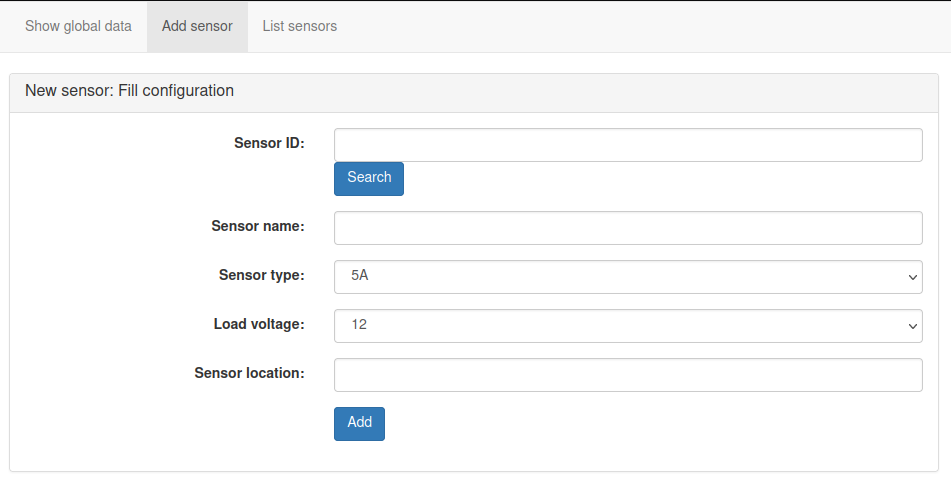
\includegraphics[width=1\textwidth]{imagenes/web_addsensor.png}
	\caption{Interfaz para añadir un sensor}
\end{figure}
\subsubsection{Mostrar sensores}
Aquí simplemente saldrá una lista de los sensores que haya configurados.
\begin{figure}[h!]
	\centering
	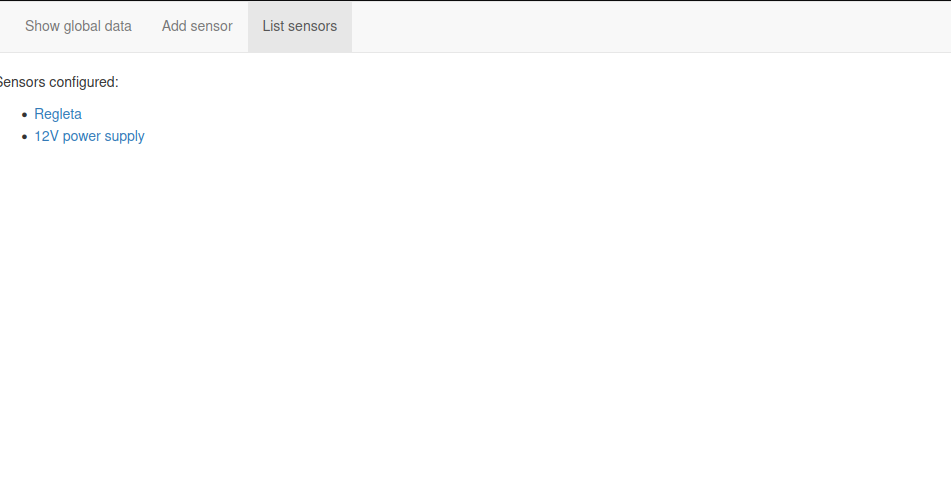
\includegraphics[width=1\textwidth]{imagenes/web_listsensors.png}
	\caption{Interfaz para mostrar los sensores añadidos}
\end{figure}
\subsubsection{Mostrar datos de un sensor}
En esta interfaz se mostrarán los datos del sensor elegido. Por un lado tenemos una grafica que va mostrando en tiempo real los datos que se van recibiendo del sensor en Watts. Por otro lado podemos ver una tabla con los datos del consumo actual, el coste en euros del consumo actual, el precio del KWh y el consumo total en KWh. Tambien tenemos un cuadro con la información del sensor y unos botones para enviar un reset al esp32, que se calibre de nuevo el sensor y para eliminar el sensor configurado. Por ultimo se muestra una especie de consola con los ultimos 20 valores recibidos del sensor. 
\begin{figure}[h!]
	\centering
	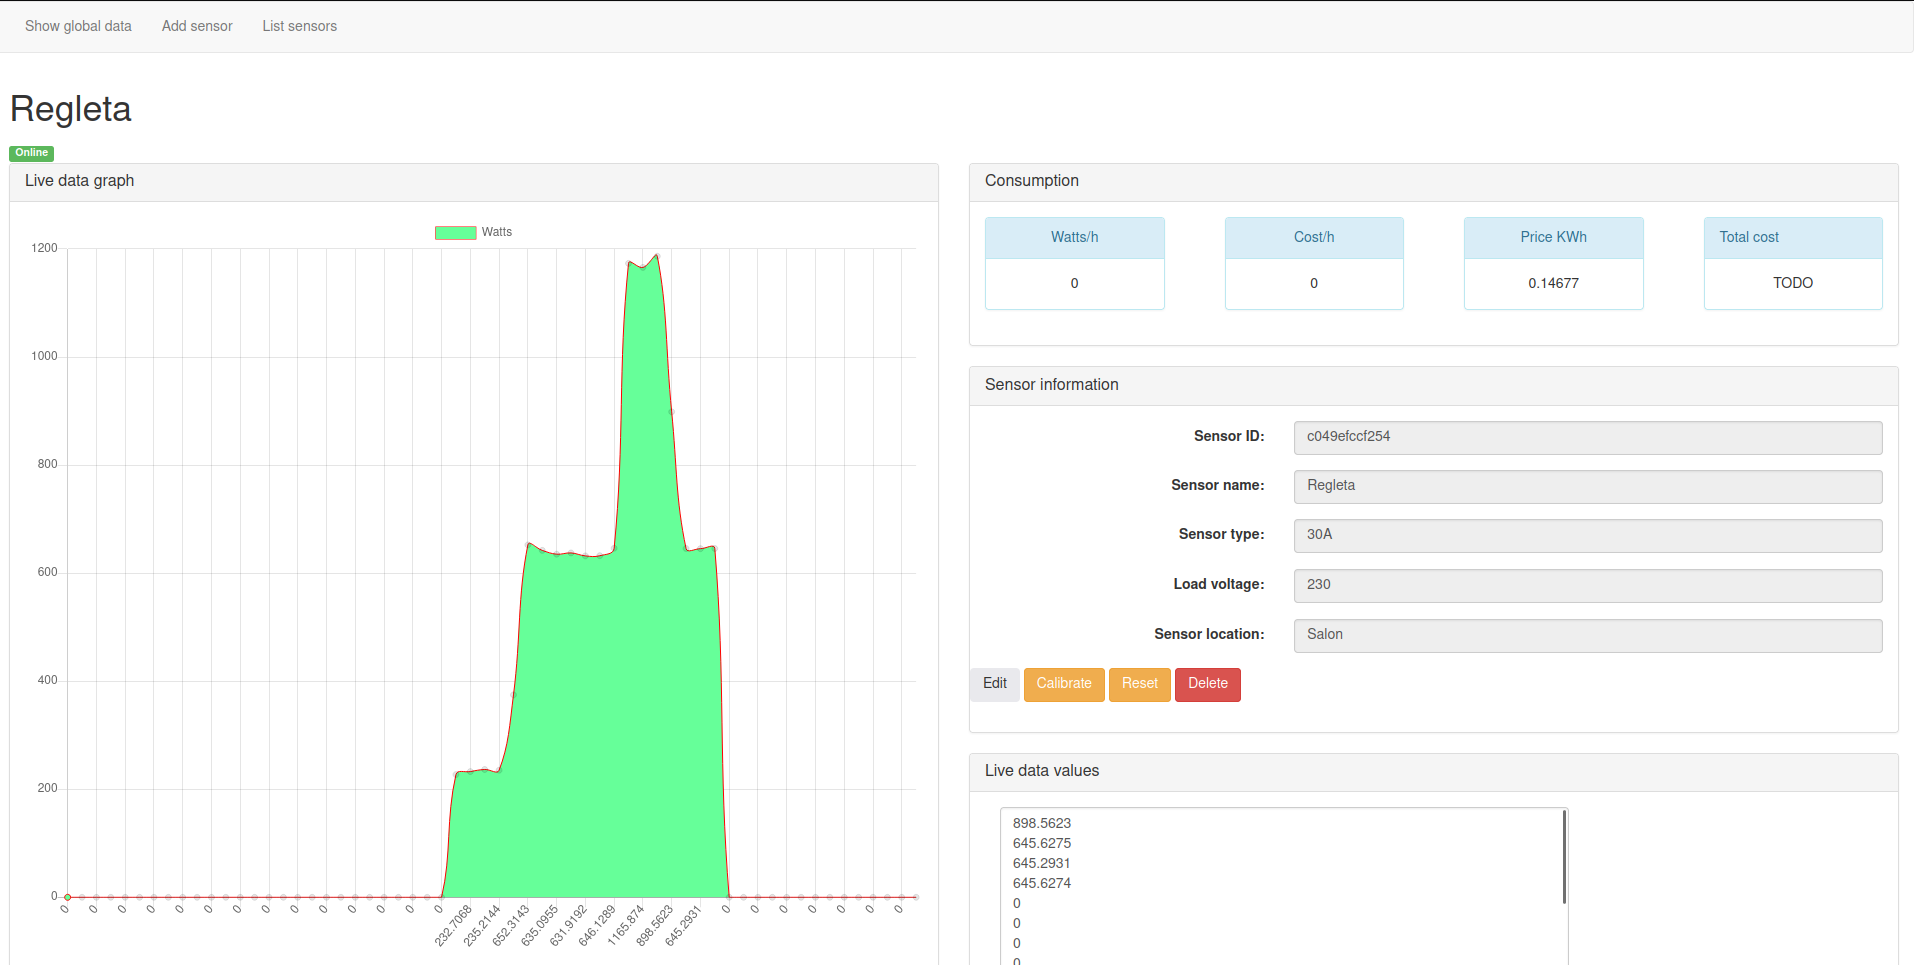
\includegraphics[width=1\textwidth]{imagenes/web_datos.png}
	\caption{Interfaz para mostrar los datos de un sensor}
\end{figure}
\subsection{Implementación}
Para la implementación del frontend se ha usado html, javascript y bootstrap. El codigo completo se puede consultar en el repositorio de GitHub\cite{ref25} en la carpeta de templates.


\end{titlepage}

%
\begin{titlepage}
\chapter{Conclusiones}
En este último capitulo vamos a recopilar todo lo aprendido en el transcurso de este proyecto, vamos a describir las conclusiones sacadas en cada uno de los escenarios en los que hemos podido probar el sistema desarrollado y vamos a hacer una valoración final del proyecto.\\
\section{Objetivos marcados}
A continuación voy a describir los objetivos marcados al inicio del proyecto y voy a indicar uno por uno si se han cumplido. Para ello lo voy a dividir en las diferentes fases en las que fue pensado inicialmente.
\subsection{Fase 1}
\begin{enumerate}
    \item Conocer en profundidad cómo funciona MicroPython
    \begin{enumerate}
        \item Conocer las limitaciones de MicroPython. \checkmark
        \item Escribir varios programas de prueba para familizarizarse con el entorno. \checkmark
    \end{enumerate}
    \item Preparar el Esp32 para poder ejecutar MicroPython.
    \begin{enumerate}
        \item Borrar flash interna. \checkmark
        \item Escribir MicroPython firmware en el microcontrolador. \checkmark
    \end{enumerate}
    \item Integrar el sensor de corriente ACS712 con el Esp32. 
    \begin{enumerate}
        \item Programa que muestre a un LCD o por consola el consumo cada segundo. \checkmark
        \item Añadir una función para encender o apagar la monitorización del sensor con un botón.\checkmark
    \end{enumerate}
\end{enumerate}

\subsection{Fase 2}
\begin{enumerate}
    \item Configurar la Raspberry Pi como broker MQTT
    \item Configurar el esp32 como publisher de MQTT.
    \begin{enumerate}
        \item Hacer una primera aproximación con un programa que publique el estado (encendido o apagado) de un led. \checkmark
        \item Integrar MQTT en el programa de la tarea anterior con el sensor de corriente. El esp32 publicará cada segundo los datos del ACS712. \checkmark
        \item Hacer que el Esp32 sea capaz de recibir órdenes de la raspberry para sustituir el botón de la primera tarea por un comando para apagar o encender la monitorización. \checkmark
        \item Estudiar la viabilidad de implementar el deep-sleep del esp32 para que no consuma nada mientras no estamos monitorizando. Estudiar las diferentes fuentes disponibles para despertar al esp32.X
    \end{enumerate}
    \item Crear aplicación temporal que muestre los datos recibidos de los diferentes publishers por la consola. \checkmark
\end{enumerate}


\subsection{Fase 3}
\begin{enumerate}
    \item Diseñar interfaz de la app web. \checkmark
    \item Mostrar en tiempo real los datos publicados por los sensores en la app web. \checkmark
\end{enumerate}


\section{Trabajo futuro}
\subsection{Mejoras en el sensor de corriente}
La primera linea de continuación de este proyecto seria comparar los resultados obtenidos con el ACS712 con otro sensor de corriente como el ZMPT101B. Aunque los resultados obtenidos con el ACS712 en comparación con el amperimetro son bastante buenos, seria interesante compararlos igualmente con otro sensor de corriente.\\

Actualmente, el sistema es tan solo un prototipo que se alimenta por USB. Para poder hacer un sistema mas real, seria necesario añadir una fuente de alimentación\cite{ref24} que convierta los 230V de corriente alterna a 5V de corriente continua.\\

Tal y como se puede leer en el datasheet del ESP32, cuando el WiFi esta encendido, se produce un ruido sobre los ADCs que puede llegar a falsear los datos de medición del consumo electrico. Por ello, seria interesante añadir un ADC externo mas preciso que no se vea afectado por el ruido del WiFi y comparar los resultados para ver si merece la pena usar el ADC externo. \\

Por último, actualmente la configuración del WiFi (SSID y contraseña) y la IP del broker MQTT estan hardcodeados en el codigo. Esto es funcional a nivel de prototipo, pero para un sistema real seria necesario poder configurar estos datos de manera remota. Para ello, se podria añadir que por defecto el ESP32 se pusiera en modo punto de acceso WiFI a la vez que lanzara un servidor web para poder configurar los datos de conexión. \\
\subsection{Mejoras en la aplicación web}
Respecto a la aplicación Web, lo principal seria añadir la funcionalidad del panel central que muestre los datos de todos los sensores a la vez. \\
Otra mejora importante seria añadir el historico de datos. Para ello deberiamos de configurar una base de datos donde guardasemos por ejemplo los datos de las ultimas 24h. De esta manera, al refrescar la pagina no deberiamos observar como perdemos los datos y solo aparecen los nuevos recibimos, si no que podriamos ver una continuación de los datos anteriores. \\

\end{titlepage}

%

\begin{thebibliography}{9}
%\chapter{Bibliografía}
%\bibitem{ts1}
%A. Mahmood, R. Exel and T. Sauter, `Impact of hard-and software timestamping on clock synchronization performance over IEEE 802.11' 2014 10th IEEE Workshop on Factory Communication Systems (WFCS 2014), Toulouse, 2014, pp. 1-8.
%doi: 10.1109/WFCS.2014.6837584. \url{http://ieeexplore.ieee.org/stamp/stamp.jsp?arnumber=6837584}
%\bibitem{ref2}
%AN-1728 IEEE 1588 Precision Time Protocol Time Synchronization Performance. Texas instruments. Revised April 2013. \url{http://www.ti.com/lit/an/snla098a/snla098a.pdf}
\bibitem{ref1}
How to measure electrical power \url{https://www.ksb.com/en-global/centrifugal-pump-lexicon/article/power-measurement-1116920}
\bibitem{ref2}
Electical waves \url{https://www.electronics-tutorials.ws/waveforms/waveforms.html}

\bibitem{ref3}
What is power factor and why is it important? \url{https://www.fluke.com/en/learn/blog/power-quality/power-factor-formula}

\bibitem{ref4}
An Explanation of RMS Power Measurement \url{https://www.electronicdesign.com/power-management/article/21120866/whats-the-difference-between-rms-and-peak-watts}

\bibitem{ref5}
INA219 Current sensor \url{https://www.ti.com/lit/ds/symlink/ina219.pdf}

\bibitem{ref6}
ZMPT101B Current sensor \url{https://datasheetspdf.com/mobile/1031464/ETC/ZMPT101B/1}

\bibitem{ref7}
ACS712 Current sensor \url{https://cdn-reichelt.de/documents/datenblatt/A200/ACS712.pdf}

\bibitem {ref8}
Arduino \url{https://www.arduino.cc/}

\bibitem {ref9}
Raspberry Pi \url{https://www.raspberrypi.org/}

\bibitem {ref10}
Esp8266 \url{https://www.espressif.com/sites/default/files/documentation/0a-esp8266ex_datasheet_en.pdf}

\bibitem {ref11}
ESP32 \url{https://www.espressif.com/en/products/socs/esp32}

\bibitem {ref12}
Micropython \url{https://micropython.org/}

\bibitem {ref13}
Ejemplo en micropython \url{https://docs.micropython.org/en/latest/esp32/quickref.html#pins-and-gpio}

\bibitem {ref14}
MQTT \url{https://mqtt.org/}

\bibitem {ref15}
Zigbee \url{https://en.wikipedia.org/wiki/Zigbee}

\bibitem {ref16}
Insight Into ESP32 Sleep Modes \& Their Power Consumption\url{https://lastminuteengineers.com/esp32-sleep-modes-power-consumption/}

\bibitem {ref17}
Esptool \url{https://docs.espressif.com/projects/esptool/en/latest/esp32/}

\bibitem {ref18}
Esptool Github \url{https://github.com/espressif/esptool}

\bibitem {ref19}
Micropython downloads \url{https://micropython.org/download/#esp32}

\bibitem {ref20}
Ampy Adafruit \url{https://learn.adafruit.com/micropython-basics-load-files-and-run-code/install-ampy}

\bibitem {ref21}
SSD1306 Micropython driver \url{https://github.com/stlehmann/micropython-ssd1306/blob/master/ssd1306.py}

\bibitem {ref22}
UMQTT.simple Micropython driver \url{https://github.com/micropython/micropython-lib/tree/master/micropython/umqtt.simple/umqtt}

\bibitem {ref23}
Enlace a proyecto en github del sensor de corriente \url{https://github.com/b0nel/TFM_CurrentSensors/tree/main/esp32}

\bibitem {ref24}
Fuente alimentación 5V \url{https://www.az-delivery.de/en/products/copy-of-220v-zu-5v-mini-netzteil}

\bibitem {ref25}
Enlace a proyecto en github de la app web \url{https://github.com/b0nel/TFM_CurrentSensors/tree/main/app_web}

\bibitem {ref26}
Imagenes de Raspbian \url{https://www.raspberrypi.com/software/operating-systems/}

\bibitem {ref27}
Etcher \url{https://www.balena.io/etcher/}

\bibitem {ref28}
Listado de broker MQTT \url{https://www.engineersgarage.com/top-mqtt-brokers-2022/}














\subsubsection{Imágenes}
\bibitem{acs712_img}
Sensor de corriente ACS712 \url{https://hifisac.com/web/image/product.template/2507/image_1024?unique=6bb2274}

\bibitem{sine_wave_img}
Forma de onda\url{https://www.electronics-tutorials.ws/wp-content/uploads/2018/05/waveforms-tim1.gif}

\bibitem{contador_img}
Contador de luz \url{https://www.google.com/url?sa=i&url=https%3A%2F%2Fwww.edistribucion.com%2Fes%2Fcontador-inteligente.html&psig=AOvVaw1P7NHoZnSfYabSYum_6eGT&ust=1669552774663000&source=images&cd=vfe&ved=0CBAQjRxqFwoTCNi_wvLuy_sCFQAAAAAdAAAAABAE}

\bibitem{factura_img}
Ejemplo de factura de la luz \url{https://www.google.com/url?sa=i&url=https%3A%2F%2Fenchufesolar.com%2Fblog%2Ftu-factura-de-la-luz-explicada-paso-a-paso%2F&psig=AOvVaw26bJ-O1gl0Srq4XB1XktT3&ust=1669552975152000&source=images&cd=vfe&ved=0CBAQjRxqFwoTCJjw99Hvy_sCFQAAAAAdAAAAABAJ}

\bibitem{medidor_img}
Enchufe medidor de consumo electrico \url{https://www.google.com/url?sa=i&url=https%3A%2F%2Fwww.elconfidencial.com%2Ftecnologia%2F2021-08-19%2Fmedidores-consumo-electrico-para-ahorrar-energia_3237006%2F&psig=AOvVaw0NNrUmh-RooxXDxCa3Y-p5&ust=1669553501475000&source=images&cd=vfe&ved=0CBAQjRxqFwoTCNCk1uHxy_sCFQAAAAAdAAAAABAD}

\bibitem{medidor_cuadro_img}
Medidor consumo cuadro electrico \url{https://www.google.com/url?sa=i&url=https%3A%2F%2Fwww.amazon.de%2F-%2Fen%2FDigital-Electricity-Top-hat-1-Phase-AC230V%2Fdp%2FB08T62R7Y5&psig=AOvVaw0SbT0RjfTplhgZSh5ESXo7&ust=1669553760554000&source=images&cd=vfe&ved=0CBAQjRxqFwoTCNim0cjyy_sCFQAAAAAdAAAAABAE}

\bibitem{monitor_inteligente_img}
Monitor de energia inteligente \url{https://www.google.com/url?sa=i&url=https%3A%2F%2Fwww.amazon.com%2F-%2Fes%2Finteligente-electricidad-Medici%25C3%25B3n-Conserva-tranquilidad%2Fdp%2FB086BNQ1X4&psig=AOvVaw1hO14UGx5ZKO99RTKsxWgl&ust=1669554058157000&source=images&cd=vfe&ved=0CBAQjRxqFwoTCLiPxdbzy_sCFQAAAAAdAAAAABAE}

\bibitem{ina219_img}
Sensor INA219 \url{https://cdn-reichelt.de/bilder/web/xxl_ws/A300/DEBO_SENS_POWER_01.png}

\bibitem{zmpt101b_img}
Sensor ZMPT101B \url{https://mvelectronica.s3.us-east-2.amazonaws.com/productos/ZMPT/60997a27ba948.webp}

\bibitem{arduino_img}
Arduino \url{https://components101.com/sites/default/files/component_pin/Arduino-Uno-Pin-Diagram.png}

\bibitem{rpi_img}
Raspberry Pi \url{https://learn.microsoft.com/en-us/windows/iot-core/media/pinmappingsrpi/rp2_pinout.png}

\bibitem{esp8266_img}
Esp8266 \url{https://components101.com/sites/default/files/component_pin/NodeMCU-ESP8266-Pinout.jpg}

\bibitem{esp32_img}
Esp32 \url{https://raw.githubusercontent.com/AchimPieters/esp32-homekit-camera/master/Images/ESP32-38%20PIN-DEVBOARD.png}

\bibitem{mqtt_img}
Ejeplo MQTT \url{https://mqtt.org/assets/img/mqtt-publish-subscribe.png}

\bibitem{zigbee_img}
Ejemplo Zigbee \url{https://csa-iot.org/wp-content/uploads/2021/12/Zigbee_SmartHome-996x1024.png}

\bibitem{voltage_divider_img}
Divisor de tension \url{https://upload.wikimedia.org/wikipedia/commons/thumb/3/31/Impedance_voltage_divider.svg/1200px-Impedance_voltage_divider.svg.png}

\bibitem{rms_voltage_equivalent_img}
Voltaje equivalente RMS \url{https://www.electronics-tutorials.ws/wp-content/uploads/2018/05/articles-rms1.gif}

\bibitem{zmpt101b_img} Sensor zmpt101b \url{https://m.media-amazon.com/images/I/61ReuklBYML._SL1190_.jpg}

\end{thebibliography}
%https://arxiv.org/pdf/1609.06771.pdf
%https://www.microsemi.com/document-portal/doc_view/133481-ptp-telecom-profiles-for-frequency-phase-and-time-synchronization
%
%
%%\nocite{*}
%\bibliography{bibliografia/bibliografia}\addcontentsline{toc}{chapter}{Bibliografía}
%\bibliographystyle{miunsrturl}
%
\appendix
%\begin{titlepage}
\chapter{Análisis de costes}
Para el análisis de los costes, me he basado en la planificación inicial (solo tendré en cuenta las horas de realización del proyecto y no las horas de realización de este documento).\\

1. En primer lugar tenemos que considerar que el trabajo de Fin de Máster cuenta como 12 ECTS, lo que debería equivaler a 300 horas de trabajo (25h por crédito). \\

2. Inicialmente se estimo un total de 43 dias (344 horas) para la realización del proyecto. Aquí ya podemos observar que no se realizó una buena planificación en cuanto a las horas disponibles para la realización del proyecto. Las 44h de más que se plantearon inicialmente tambien las tendré en cuenta.\\

3. El coste de trabajo de cada hora, para un ingeniero informático con experiencia y en base a la experiencia que tengo en el mercado laboral, consideraré un coste por hora de 20 euros brutos, lo que supone un coste salarial de 20\euro /h x 344h = 6880\euro.\\

4. Si considerasemos este proyecto para su realización como algo profesional, deberiamos entonces considerar algunos costes indirectos relacionados con el desarrollo de la actividad, tales como agua, luz, conexión a internet, alquiler de equipos, etc. A grosso modo podriamos estimar unos 1200 euros.\\

5. Para la realización de este proyecto, el uso del equipo informatico para el desarrollo e investigación del proyecto tambien se ha de tener en cuenta. Para cada uno de ellos se calcula el coste estableciendo su vida útil y el tiempo de uso como variables que lo componen. Se supone, para todos, una vida útil de 36 meses y un tiempo de uso de 6 meses. La proporción a seguir es (Meses uso / Vida útil) * Coste de Adquisición.\\

Ordenador de sobremesa: 
\begin{itemize}
	\item Precio Adquisición = 2.000 \euro
	\item Coste = 333 \euro
\end{itemize}

Raspberry: 
\begin{itemize}
	\item Precio Adquisición = 40 \euro
	\item Coste= 7 \euro 
\end{itemize}

Ubuntu: 
\begin{itemize}
	\item Precio Adquisición = 0 \euro
	\item Coste= 0 \euro  
\end{itemize}

Raspbian OS: 
\begin{itemize}
	\item Precio Adquisición = 0 \euro
	\item Coste= 0 \euro  
\end{itemize}

Fuente de alimentación: 
\begin{itemize}
	\item Precio Adquisición = 150 \euro
	\item Coste= 25 \euro  
\end{itemize}

Subtotal: 365 \euro

6. Para los componentes electronicos, consideramos su precio de adquisición como coste total.\\

Sensores ACS712 5A:
\begin{itemize}
	\item Coste=  13\euro  
\end{itemize}

Sensores ACS712 30A:
\begin{itemize}
	\item Coste=  13\euro  
\end{itemize}

Sensores ZMPT101B:
\begin{itemize}
	\item Coste=  24\euro  
\end{itemize}

Microcontroladores ESP32:
\begin{itemize}
	\item Coste=  28\euro  
\end{itemize}

Caja de resistencias:
\begin{itemize}
	\item Coste=  15\euro  
\end{itemize}

Caja de condensadores:
\begin{itemize}
	\item Coste=  10\euro  
\end{itemize}

Reles:
\begin{itemize}
	\item Coste=  12\euro  
\end{itemize}

Subtotal: 115 \euro \\

Sumando todo, el coste total del desarrollo del proyecto se podria estimar en: \\

Salario: 6880\euro

Costes indirectos: 1200\euro

Coste de equipos: 365\euro

Coste de hardware electronico: 115\euro

TOTAL: 8560 \euro


\end{titlepage}
%%\input{apendices/paper/paper}
%\input{glosario/entradas_glosario}
% \addcontentsline{toc}{chapter}{Glosario}
% \printglossary
\chapter*{}
\thispagestyle{empty}

\end{document}
